%%%%%%%%%%%%%%%%%%%%%%%%%%%%%%%%%%%%%%%%%
% Thesis Template
% LaTeX Template
% Version 1.5.1 (2024-02-20)
%
% This template was adapted by:
% Lars Quentin (lars.quentin@stud.uni-goettingen.de) and
% Jonathan Decker (jonathan.decker@uni-goettingen.de)
% Adapted from the informatics master and bachelor thesis template
% offered by the University Göttingen
% https://www.uni-goettingen.de/de/626775.html
%
%%%%%%%%%%%%%%%%%%%%%%%%%%%%%%%%%%%%%%%%%

% !TEX root = main.tex

% --- document configuration ---

%cf-ignore-acro-begin

\newcommand{\thesistitle}{Evaluation of Ceph as a File~System~for~HPC}
\newcommand{\firstsupervisor}{Dr. Julian Kunkel}
\newcommand{\secondsupervisor}{Dr. Sebastian Krey}
\newcommand{\authorname}{Tim Dettmar}
\newcommand{\university}{Georg-August-Universität Göttingen}
\newcommand{\department}{Institute of Computer Science}
\newcommand{\thesistype}{Master's Thesis} % Bachelor's Thesis or Master's Thesis
\newcommand{\course}{Applied Computer Science}
\newcommand{\matrikelnumber}{26327113}
\newcommand{\keywords}{Ceph} % Set keywords that describe your report
\newcommand{\documentlanguage}{en-US} % Required for PDF/A
\newcommand{\submissiondate}{\today}

% --- PDF/A compliance ---
% Taken from the template provided by the Institute of Informatics, University of Goettingen
\pdfminorversion=7
\begin{filecontents*}{\jobname.xmpdata}
	\Title{\thesistitle}
	\Author{\authorname}
	\Language{\documentlanguage}
	\Subject{The abstract, or short description}
	\Keywords{\keywords}
\end{filecontents*}

\documentclass[12pt, a4paper, hidelinks]{article}

% \usepackage{subfig}
\usepackage{enotez}
\usepackage{adjustbox}
\usepackage{graphicx}
\usepackage{hyperref}
\usepackage{xcolor}
\usepackage[english,british]{babel}
\usepackage[nottoc]{tocbibind}
\usepackage[utf8]{inputenc}
\usepackage[T1]{fontenc}
\usepackage{pgfplots}
\usepackage{caption}
\usepackage{subcaption}
\usepackage[backend=biber,style=alphabetic]{biblatex}
\addbibresource{ref.bib} % The filename of the bibliography
\usepackage[left=2.5cm,right=2.5cm,top=2.5cm,bottom=2.5cm]{geometry}
\usepackage{acronym}
\usepackage{fancyhdr}
\pagestyle{fancy}
\usepackage{lipsum}
\usepackage{array, tabularx, booktabs} % For better tables
\usepackage{longtable}
\usepackage{xurl}

\usepackage{marvosym} % For Telephone, fax and Letter symbols
\usepackage{listings} % Code environments
\usepackage{lstautogobble}  % Fix relative indenting
\usepackage{color}          % Code coloring
\usepackage{zi4}            % Nice font
\usepackage{minted}
\usemintedstyle{tango}
\setminted{linenos, autogobble, bgcolor=gray!5}
\usepackage{amsmath}
\usepackage{cleveref}
\usepackage{titlesec}
\setlength{\marginparwidth}{2cm}
\usepackage{todonotes}
\usepackage[autostyle=true]{csquotes}
\usepackage{multirow}
\usepackage{diagbox}
\usepackage{xfrac}
\usepackage{subcaption}

\usepackage{pdflscape}
\usepackage{afterpage}
\usepackage{wrapfig}
\usepackage{floatflt}
\usepackage{placeins}

\usepackage{markdown}

\definecolor{codegreen}{rgb}{0,0.6,0}
\definecolor{codegray}{rgb}{0.5,0.5,0.5}
\definecolor{backcolour}{gray}{0.95}
\definecolor{codeorange}{rgb}{0.8,0.5,0.2}

\lstdefinestyle{mystyle}{
    backgroundcolor=\color{backcolour},  
    commentstyle=\color{codegray},
    keywordstyle=\color{codeorange},
    numberstyle=\tiny\color{codegray},
    stringstyle=\color{codegreen},
    basicstyle=\ttfamily\footnotesize,
    breakatwhitespace=false,         
    breaklines=true,                 
    captionpos=b,                    
    keepspaces=true,                 
    numbers=left,                    
    numbersep=20pt,                  
    showspaces=false,                
    showstringspaces=false,
    showtabs=false,                  
    tabsize=2,
    linewidth=.9725\textwidth,
}

\lstset{style=mystyle}

\definecolor{bluekeywords}{rgb}{0.13, 0.13, 1}
\definecolor{greencomments}{rgb}{0, 0.5, 0}
\definecolor{redstrings}{rgb}{0.9, 0, 0}
\definecolor{graynumbers}{rgb}{0.5, 0.5, 0.5}

\lstset{
    autogobble,
    columns=fullflexible,
    showspaces=false,
    showtabs=false,
    breaklines=true,
    showstringspaces=false,
    breakatwhitespace=true,
    escapeinside={(*@}{@*)},
    commentstyle=\color{greencomments},
    keywordstyle=\color{bluekeywords},
    stringstyle=\color{redstrings},
    numberstyle=\color{graynumbers},
    basicstyle=\ttfamily\footnotesize,
    frame=l,
    framesep=12pt,
    xleftmargin=12pt,
    tabsize=4,
    captionpos=b
}

\lstdefinelanguage{ini}{
    basicstyle=\ttfamily\small,
    columns=fullflexible,
    morecomment=[l]{\#},
    morecomment=[l]{;},
    commentstyle=\color{gray},
    stringstyle=\color{red},
    keywordstyle=\color{blue}\bfseries,
    identifierstyle=\color{black},
}

\titleformat{\section}[hang]{\huge\bfseries}{\thesection\hspace{20pt}}{0pt}{\huge\bfseries}
\graphicspath{{Figures/}{./}{Assets/}}

\newcommand{\ccheckmark}{\mbox{\ooalign{$\checkmark$\cr\hidewidth$\square$\hidewidth\cr}}}
\newcommand{\ccheckbox}{\mbox{$\square$}}

\newcommand{\addemptypage}{\newpage\null\thispagestyle{empty}\newpage}

\begin{document}

\fancyhead{}
\fancyhead[R]{\footnotesize \thesistitle}
\fancyfoot{}
\fancyfoot[R]{\thepage}
\fancyfoot[L]{Section \thesection}
\fancyfoot[C]{\authorname}
\renewcommand{\headrulewidth}{0.4pt}
\renewcommand{\footrulewidth}{0.4pt}

\pagestyle{empty}
\hypersetup{pageanchor=false} %Avoid issue with invisible numbering style
% --- title page ---

\begin{titlepage}

\includegraphics[width=6.5cm]{assets/logo-goettingen.pdf} \hfill 
\includegraphics[width=2.5cm]{assets/hps-logo.pdf}
	
\begin{center}
	
	\vspace*{.06\textheight}
	{\LARGE \textbf{\thesistype}\\}
	submitted in partial fulfillment of the\\
	requirements for the course ``\course''\\[0.5cm]
	
	
	\rule{.9\linewidth}{.6pt} \\[0.4cm] % Horizontal line
	{\huge \bfseries \thesistitle}\vspace{0.4cm}
	\rule{.9\linewidth}{.6pt} \\[1.5cm] % Horizontal line
	
	\Large\authorname\\
	\hfill\\
	\large MatrNr: \matrikelnumber\\ \vfill
	\begin{tabular}{@{}ll}
		First Supervisor: &\firstsupervisor\\
		Second Supervisor: &\secondsupervisor
	\end{tabular}
	\vfill
	\university\\
	\department\\
	ISSN: 1612-6793
	\vfill
	{\large \submissiondate}\\[4cm] % Date
	
	\vfill
\end{center}

\newpage
\vfill

\input{contact}


\end{titlepage}

% --- abstract ---

\newpage
\pagenumbering{roman}
\setcounter{page}{1}

\section*{Abstract}
\ac{HPC} workloads place high demands on storage systems, requiring them to reliably provide high throughput for a wide variety of data access patterns. However, data access patterns in \ac{HPC} are varied, introducing unique architectural challenges. Ceph, a distributed and flexible software-defined storage system, has historically seen limited adoption in the \ac{HPC} space, with incumbent file systems such as Lustre and BeeGFS dominating the market. 

In this thesis, we evaluate the suitability of Ceph as a storage system for a range of data access patterns representative of those found in \ac{HPC} workloads, analyzing its performance, architectural overhead, scalability, and suitability for use in \ac{HPC} environments. To isolate the overhead of Ceph's software architecture from the bottlenecks of physical storage media, we have developed a custom, rootless deployment framework leveraging Apptainer and Slurm for the deployment of ephemeral, in-memory Ceph clusters on standard \ac{HPC} cluster nodes as well as a benchmarking framework for the automated gathering of scaling performance results with \acs{IOR} and mdtest.

Our empirical findings show that Ceph demonstrates strong scaling performance for data-heavy workloads, while its performance for metadata-heavy workloads exhibits inconsistent scaling and high variance, with performance bottlenecks and architectural limitations becoming apparent during our testing at scale. During testing, we additionally traced intermittent node crashes on the Omni-Path network fabric to a known kernel vulnerability, which had been incorrectly classified as not affecting \ac{RHEL} 8, leading to a security patch for the affected kernel. Our findings ultimately suggest that, while Ceph is highly flexible and generally a capable distributed file system for many \ac{HPC} workloads, specific limitations related to its metadata performance and current networking implementation may make it less suitable for certain \ac{HPC} use cases. However, further testing is required with physical storage devices to fully evaluate its suitability for use in \ac{HPC} environments.

\newpage

\vfill

% Fill out the statement by setting \ccheckbox for points that do not apply and \ccheckmark for points that do apply

\subsection*{Declaration on the use of ChatGPT and comparable tools\\ in the context of examinations}
\noindent In this work I have used ChatGPT or another AI as follows:
\begin{itemize}
	\item[\ccheckbox] Not at all
	\item[\ccheckmark] During brainstorming
	\item[\ccheckmark] When creating the outline
	\item[\ccheckmark] To write individual passages, altogether to the extent of 5\% of the entire text % Set the percentage if this point applies
	\item[\ccheckmark] For the development of software source texts
	\item[\ccheckmark] For optimizing or restructuring software source texts
	\item[\ccheckmark] For proofreading or optimizing
	\item[\ccheckmark] Further, namely: 
    \begin{itemize}
        \item Formatting of tables and figures into \LaTeX {}{} syntax
        \item Debugging code
        \item Generating and fixing Plotly code to extract collected data for charts
        \item Generation of code for detecting and fixing of thesis formatting issues
    \end{itemize}
\end{itemize}
I hereby declare that I have stated all uses completely.\\
Missing or incorrect information will be considered as an attempt to cheat.


\vfill

\newpage

%cf-ignore-acro-end

\section*{Acknowledgements}

I would like to express my gratitude to my supervisors, Julian Kunkel and
Jonathan Decker, for their guidance, support, and feedback throughout this
thesis.

I am also thankful to the \ac{GWDG} for providing access to their computing
infrastructure as well as the generous core-hour allocations necessary to
perform the large-scale tests that made the thesis possible.

Furthermore, I would like to thank my family and friends for their encouragement
and support during the many long and challenging phases of this work.

Last but not least, I would like to acknowledge an anonymous participant of the
Chaos Communication Congress, whose willingness to lend their time sharing their
practical knowledge and experience guided me towards identifying and resolving
particularly peculiar bugs within my Ceph setup.

\newpage
\pagestyle{plain}
% --- table of contents ---
% Comment out the lists you are not using
\clearpage
% if you have abbreviations
% !TEX root = main.tex

\newpage
%cf-ignore-acro-begin
\section*{List of Abbreviations} \addcontentsline{toc}{section}{List of Abbreviations}
% Add acronyms such that they are shown in full only on first occurrence
% I am not screaming, this is just for spacing
\begin{acronym}[AAAAAAA] 
    \acro{AI}{Artificial Intelligence}
    \acro{API}{Application Programming Interface}
    \acro{CephFS}{Ceph Filesystem}
    \acro{CLI}{Command-Line Interface}
    \acro{CPU}{Central Processing Unit}
    \acrodefplural{CPU}{Central Processing Units}
    \acro{CRUSH}{Controlled Replication Under Scalable Hashing}
    \acro{CSV}{Comma-Separated Values}
    \acro{DDF}{Disk Data Format}
    \acro{DMA}{Direct Memory Access}
    \acro{DPDK}{Data Plane Development Kit}
    \acro{DRAM}{Dynamic Random Access Memory}
    \acro{EC}{Erasure Coding}
    \acro{EOS}{EOS Open Storage}\footnote{Recursive acronym}
    \acro{ER}{Entity-Relationship}
    \acro{FIO}{Flexible I/O Tester}
    \acro{FLR}{File-Level Redundancy}
    \acro{FUSE}{Filesystem in Userspace}
    \acro{GPU}{Graphics Processing Unit}
    \acro{GRO}{Generic Receive Offload}
    \acro{GSO}{Generic Segmentation Offload}
    \acro{GUI}{Graphical User Interface}
    \acro{GWDG}{Gesellschaft für wissenschaftliche Datenverarbeitung mbH Göttingen}
    \acro{HA}{High Availability}
    \acro{HDD}{Hard Disk Drive}
    \acrodefplural{HDD}{Hard Disk Drives}
    \acro{HPC}{High-Performance Computing}
    \acro{I/O}{Input/Output}
    \acro{IB}{InfiniBand}
    \acro{IO}{Input/Output}
    \acro{IOMMU}{I/O Memory Management Unit}
    \acro{IOPS}{Input/Output Operations Per Second}
    \acro{IOR}{Interleaved or Random}
    \acro{IP}{Internet Protocol}
    \acro{IPoIB}{Internet Protocol Over InfiniBand}
    \acro{IRQ}{Interrupt Request}
    \acro{JSON}{JavaScript Object Notation}
    \acro{LLM}{Large Language Model}
    \acro{LLNL}{Lawrence Livermore National Laboratory}
    \acro{LVM}{Logical Volume Management}
    \acro{MBGD}{Mini-Batch Gradient Descent}
    \acro{MDS}{Metadata Server}
    \acrodefplural{MDS}{Metadata Servers}
    \acro{ML}{Machine Learning}
    \acro{MLC}{Multi-Level Cell}
    \acro{Mon}{Monitor}
    \acrodefplural{Mon}{Monitors}
    \acro{MPI}{Message Passing Interface}
    \acro{MTU}{Maximum Transmission Unit}
    \acro{NFS}{Network File System}
    \acro{NUMA}{Non-Uniform Memory Access}
    \acro{NVMe}{Non-Volatile Memory Express}
    \acro{NVMeoF}{Non-Volatile Memory Express over Fabrics}
    \acro{NVRAM}{Non-Volatile Random Access Memory}
    \acro{OCI}{Open Container Initiative}
    \acro{ORNL}{Oak Ridge National Laboratory}
    \acro{OS}{Operating System}
    \acro{OSD}{Object Storage Daemon}
    \acrodefplural{OSD}{Object Storage Daemons}
    \acro{OST}{Object Storage Target}
    \acro{PG}{Placement Group}
    \acrodefplural{PG}{Placement Groups}
    \acro{PoC}{Proof of Concept}
    \acro{POSIX}{Portable Operating System Interface}
    \acro{PSM}{Performance Scaled Messaging}
    \acro{QLC}{Quad-Level Cell}
    \acro{RADOS}{Reliable Autonomic Distributed Object Store}
    \acro{RAID}{Redundant Array of Independent Disks}
    \acro{RAM}{Random Access Memory}
    \acro{RBD}{RADOS Block Device}
    \acro{RDMA}{Remote Direct Memory Access}
    \acro{RGW}{RADOS Gateway}
    \acro{RHEL}{Red Hat Enterprise Linux}
    \acro{RPS}{Receive Packet Steering}
    \acro{S3}{Simple Storage Service}
    \acro{SAN}{Storage Area Network}
    \acrodefplural{SAN}{Storage Area Networks}
    \acro{SAS}{Serial Attached SCSI}
    \acro{SATA}{Serial AT Attachment}
    \acro{SDMA}{Send Direct Memory Access}
    \acro{SIF}{Singularity Image Format}
    \acro{SLC}{Single-Level Cell}
    \acro{SLES}{SUSE Linux Enterprise Server}
    \acro{SNIA}{Storage Networking Industry Association}
    \acro{SPDK}{Storage Performance Development Kit}
    \acro{SSD}{Solid-State Drive}
    \acrodefplural{SSD}{Solid State Drives}
    \acro{SSH}{Secure Shell}
    \acro{TCP}{Transmission Control Protocol}
    \acro{TCP/IP}{Transmission Control Protocol over Internet Protocol}
    \acro{THP}{Transparent Huge Pages}
    \acro{TLC}{Triple-Level Cell}
    \acro{UDP}{User Datagram Protocol}
    \acro{USB}{Universal Serial Bus}
    \acro{VM}{Virtual Machine}
    \acrodefplural{VM}{Virtual Machines}
\end{acronym}
%cf-ignore-acro-end

\thispagestyle{plain}
\newpage

\phantomsection\pdfbookmark{\contentsname}{toc}
\tableofcontents

\newpage
\clearpage\phantomsection
\listoftables
\newpage
\clearpage
\phantomsection
\listoffigures
\newpage
\clearpage
\phantomsection
\listoflistings \addcontentsline{toc}{section}{List of Listings}
\newpage

% --- content ---

\hypersetup{pageanchor=true}
\pagenumbering{arabic}
\setcounter{page}{1}
\pagestyle{fancy}

% !TEX root = main.tex

\section{Introduction}

\subsection{Motivation}

Storage plays an important role in \ac{HPC} environments, with demands on storage infrastructure increasing steadily as modern workloads continue to grow. In addition to capacity, fast and low-latency access to data ensure that compute nodes can spend more time on computation tasks rather than waiting for data, increasing compute efficiency. Given that \ac{HPC} clusters' resources are often shared among multiple users, file systems should also be able to handle requests from multiple users with an acceptable level of performance.

Incumbents in the \ac{HPC} space, such as Lustre, are designed specifically to be \ac{HPC} file systems~\cite{lustre-homepage}. This allows for the design of the file system to be highly optimized for these use cases, with a proven track record and market share over time. However, this highly optimized nature presents issues in terms of hardware complexity and cost, as well as maintainability, due to the rigid requirements of these file systems.

Ceph emerges from this background as a potentially compelling alternative to incumbent file systems due to its flexible design. It is a fully software-defined, distributed storage system, designed to be a ``catch-all'' solution---with the express intent of being deployable on commodity hardware, while maintaining flexibility for larger deployments. However, Ceph has not yet seen wide deployment in the \ac{HPC} space, with \acs{HPC}-specific file systems still making up the majority of the backing storage for supercomputers in the IO500 rankings for storage performance~\cite{io500-full-list}, as shown in \Cref{fig:io500-storage-share}.

\begin{figure}[H]
    \centering
    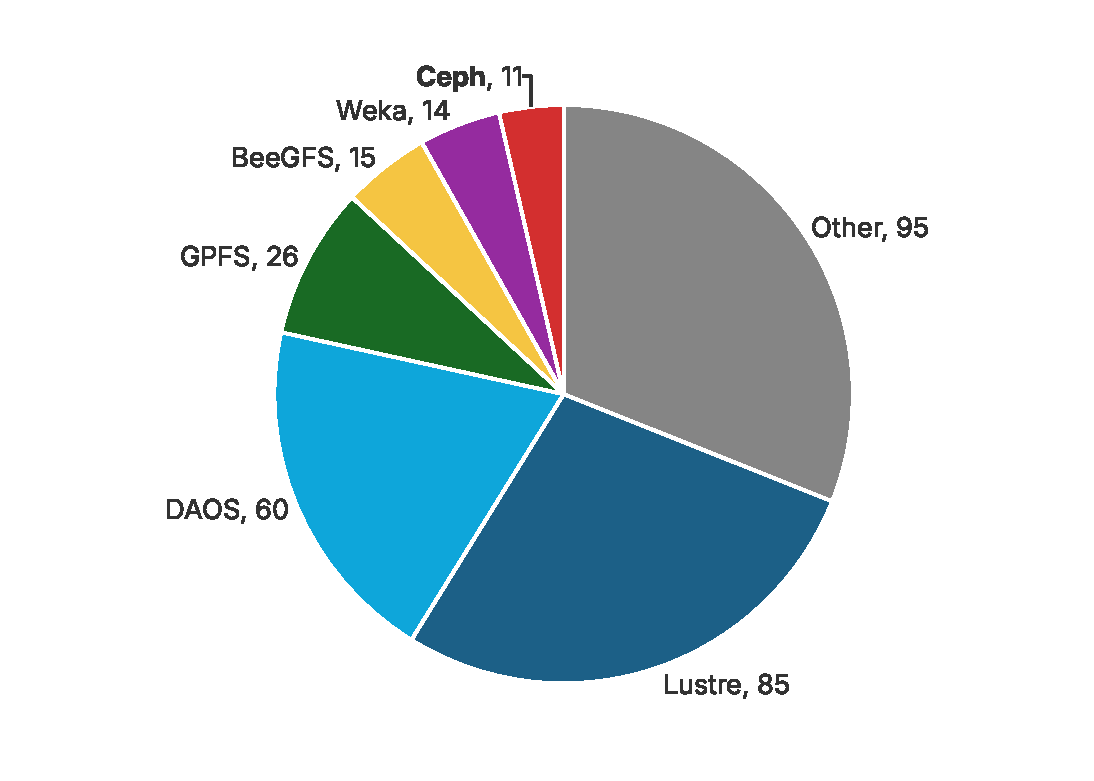
\includegraphics[height=9cm]{assets/charts/storage_market_share.pdf}
    \caption[File System Share of IO500 Results]{The share of file systems used in the IO500 rankings for storage performance~\cite{io500-full-list}}
    \label{fig:io500-storage-share}
\end{figure}

While the IO500 rankings are far from a benchmark of every \ac{HPC} system in existence, it still roughly demonstrates that file systems designed specifically for \ac{HPC} make up the majority of file systems used. Additionally, Ceph did not reach the top 100 of all historical IO500 rankings, although it did achieve 42nd place in the production-grade node list as of March 2026.

Nevertheless, it has been demonstrated that Ceph is capable of achieving 1 TiB/s of throughput in certain scenarios~\cite{ceph-1tib}. If these performance figures were reproducible under the conditions stipulated by the IO500, this would significantly improve Ceph's position in the rankings, showing at least theoretically that Ceph is capable of \ac{HPC}-class performance.

Throughout its lifetime, Ceph has also undergone several architectural changes and improvements, which necessitates a new evaluation of its performance characteristics. Initial implementations relied on a storage backend built on top of a traditional file system, introducing significant overhead and limiting performance. However, modern Ceph versions interface directly with disks, bypassing many of the architectural limitations of initial Ceph versions. Furthermore, Ceph continues to advance towards better support for high-performance networking and storage through its use of the \ac{DPDK} and \ac{SPDK} frameworks respectively, making the system's performance characteristics potentially more attractive for \ac{HPC} use cases. Given the rapid pace of development and mature software support from large vendors such as Red Hat\footnote{\url{https://www.redhat.com/en/technologies/storage/ceph}. Accessed 01.03.2026.}, re-evaluating Ceph's performance in an \ac{HPC} context is of particular interest.

\subsection{Goals}

The overarching goals of this thesis are to evaluate the viability of the Ceph storage system as a file system for \ac{HPC} workloads. Since Ceph's primarily software-defined architecture differs significantly from traditional \ac{HPC} storage solutions, we will evaluate Ceph from both the end-user and system administrator perspectives. In order to evaluate performance and scalability, the thesis pursues the following goals:

\begin{itemize}
    \item Quantification of Ceph's architectural overhead by eliminating physical disk bottlenecks where possible, isolating the overhead of Ceph's internal object and file storage abstraction layers. The quantification includes a comparison of Ceph's underlying \acs{RADOS} object storage interface, as well as its layer for serving a traditional file system (\acs{CephFS}).
    \item Evaluation of scalability with \ac{HPC} access patterns through the use of standard \ac{HPC} benchmarking tools, benchmarking various numbers of clients and file/object access patterns.
    \item Evaluation of Ceph on top of various network fabrics and protocols in order to identify bottlenecks specific to Ceph's networking implementation.
    \item Analysis of performance trade-offs introduced by Ceph's software-defined replication protocols, including standard replication and erasure-coding implementations.
\end{itemize}

In order to evaluate system administration, the thesis pursues the following:

\begin{itemize}
    \item Evaluation of Ceph's flexibility through rootless deployment on standard \ac{HPC} cluster nodes using Apptainer and Slurm with a custom-developed orchestration tool.
    \item Evaluation of Ceph's standard deployment tools for production-grade deployments, including setup complexity, recovery, and maintainability.
\end{itemize}

Overall, we aim to rigorously test Ceph in order to identify its strengths and weaknesses, as well as to uncover potential operational limitations, hardware compatibility issues, and other architectural bottlenecks, which may complicate Ceph's deployment in an \ac{HPC} environment, and provide recommendations for deployments as well as future improvements to the system.

\subsection{Contributions}

In this thesis, the main contributions are as follows:

\begin{itemize}
    \item Holistic evaluation of the Ceph file system's design and suitability for \ac{HPC} workloads
    \item A deployment and benchmarking framework designed for Ceph in \ac{HPC}, including:
    \begin{itemize}
        \item Flexible, rootless scripts for the deployment of Ceph clusters on varying \ac{HPC} compute nodes
        \item Automated scripts for performance benchmarking across various node and client configurations, usable for file systems beyond Ceph
    \end{itemize}
    \item Ceph performance analysis across clusters and client configurations of various sizes to approximate real-world deployments
    \item Identification of architectural limitations within Ceph
    \item Identification of limitations with the test hardware, which affected the gathered performance results
    \item Identification of a known kernel vulnerability\footnote{CVE-2024-26766} in the Omni-Path networking driver, which was incorrectly classified as not affecting \ac{RHEL} 8, resulting in intermittent node failures during benchmark testing
    \item A discussion of potential improvements based on the collected results and evaluations
\end{itemize}

\subsection{Structure}

The structural organization of this thesis is as follows:

\begin{itemize}
    \item \Cref{sec:background} covers the concepts essential to \ac{HPC} storage and how it relates to Ceph, followed by an overview of the Ceph architecture itself.
    \item \Cref{sec:literature-review} covers the existing literature in the field as well as potential challenges of benchmarking Ceph, especially in an \ac{HPC} context.
    \item \Cref{sec:methodology} details the cluster deployment and benchmarking system developed for this thesis, as well as the test systems used to perform the benchmarking.
    \item \Cref{sec:results} reports the benchmark findings.
    \item \Cref{sec:discussion} interprets the results, discusses the limitations of our benchmarks, and determines Ceph's potential in \ac{HPC}. Additional improvements, both to Ceph itself and the benchmarking methodology are also discussed.
    \item \Cref{sec:future-work} discusses potential future work.
    \item \Cref{sec:conclusion} concludes the thesis with a summary of the findings.
\end{itemize}

\newpage
\section{Background}
\label{sec:background}

\subsection{Overview}

The question of how well Ceph performs as a file system in \ac{HPC} can be divided into two problems. We first need to answer the question of what storage is actually needed and used for in the high-performance computing sector. The findings from this initial question define the framework for the demands placed on file systems by \ac{HPC} users, which can then be used to determine benchmarking methods suitable for file system testing. Although the focus will be on Ceph in this thesis, the goal is for the work performed in this thesis, especially with regard to evaluation and benchmarking, to be applicable to other parallel file systems that may also be under consideration.

In this section, the groundwork for the rest of the thesis will be laid out by covering the fundamental concepts of file systems and how they relate to \ac{HPC}. Relevant existing literature on the topic of metrics for \ac{HPC} file systems as well as Ceph in particular will additionally be covered. 

\subsection{File Systems}

Before focusing on Ceph specifically, this section will introduce the basic concepts behind file systems and their relevance.

At the lowest level, data are typically stored on disks, be it \acp{HDD}, \acp{SSD}, or other technologies~\cite[ch.~4]{modern-operating-systems-book}. These present themselves to the operating system as \enquote{block devices}, which are arrays of fixed-size \enquote{blocks} (e.g., 4\,kilobytes). The operating system reads and writes raw binary data by addressing individual blocks. At this level, there are no filenames, folders, or other high-level abstractions.

A subset of file systems known as disk-based file systems are developed on top of these block devices. These organize the data on the disks, provide a hierarchical storage layout (i.e., folders), and provide a range of other abstractions, such as access control, checksumming, and redundancy. The exact feature set depends on the file system. These file systems are used in every major operating system, including Windows, macOS, and Linux.

When scaling up to meet \ac{HPC} demands, the performance and capacity requirements exceed the capabilities of a single server. Parallel or distributed file systems address this limitation---in contrast to local file systems (ext4, XFS, ZFS, etc.) which communicate directly with block devices, distributed file systems store data across the disks of multiple storage nodes, scaling both performance and capacity. Clients access the file system over the network, and the file system's metadata services manage file and directory operations across the cluster.

There are several parallel file systems, such as Lustre, BeeGFS, and DAOS, which are specifically targeted towards \ac{HPC} use cases\footnote{\url{https://www.lustre.org}, \url{https://www.beegfs.io}, \url{https://daos.io}. Accessed 01.03.2026.}. However, there are more general-purpose distributed file systems, including Ceph, which have seen limited adoption in \ac{HPC}, despite their widespread use outside of it.

\subsection{\acs{RAID}}
\label{sec:raid}

Storage devices are subject to constraints in performance and reliability. For example, Backblaze~\cite{backblaze-drive-stats}, a cloud storage provider, reported an annualized drive failure rate of 1.3\%. \ac{RAID} addresses these limitations by combining multiple disks to improve performance and/or reliability~\cite{raid-paper}. Several \ac{RAID} levels exist---we will cover the levels 0, 1, 5 and 6 in this overview, based on the definitions provided by the \acl{SNIA}~\cite{snia-ddf}.

The most basic levels are \ac{RAID}~0 and \ac{RAID}~1. \ac{RAID}~0 stripes data across disks, multiplying both throughput and capacity by the number of disks but providing no fault tolerance---the loss of any single disk results in data loss. \acs{RAID}~1 increases the resiliency of data storage by mirroring data across disks, such that the array remains functional as long as at least one disk survives, at the cost of capacity being limited to a single disk's size.

\begin{wrapfigure}{l}{0.4\textwidth}
    \centering
    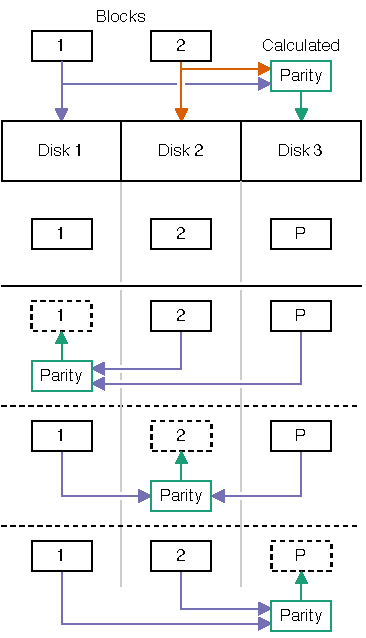
\includegraphics[width=\linewidth]{assets/raid/RAID5.pdf}
    \caption[\acs{RAID} 5 Configuration]{Data distribution across disks in a \acs{RAID} 5 configuration, demonstrating how data can be reconstructed after a single-disk failure through parity calculations.}
    \label{fig:raid5}
\end{wrapfigure}

\noindent\ac{RAID} 5 (see \cref{fig:raid5}) and \ac{RAID}~6 offer a middle ground by striping data together with parity information across disks. \ac{RAID}~5 uses single parity and can tolerate one disk failure, while \ac{RAID}~6 uses double parity for two-failure tolerance. Compared to mirroring, parity \ac{RAID} provides significantly better storage utilization---a 3-disk \ac{RAID}~5 achieves $\frac{2}{3}$ efficiency versus 50\% for a 2-disk mirror---at the expense of additional compute overhead for parity calculations. These levels can scale to larger disk counts, though the probability of an additional failure during recovery increases accordingly.

The aforementioned levels may also be combined by nesting, such as in \ac{RAID}~10, which combines \ac{RAID}~1 and \ac{RAID}~0 to provide both fault tolerance and performance. For example, a 4-disk \ac{RAID}~10 array may be considered as a \ac{RAID}~0 across two \ac{RAID}~1 sub-arrays.

The Lustre file system effectively implements \ac{RAID}~0~\cite[p.~11]{lustre-manual}, striping data across multiple disks to improve performance. However, because \ac{RAID}~0 does not provide any fault tolerance, Lustre relies on the underlying file system, such as ZFS, to provide fault tolerance with another \ac{RAID} level, such as \ac{RAID} levels 1, 5, or 6, or 10~\cite[p.~16]{lustre-manual}.

While these standard \ac{RAID} levels are widely implemented across both software and hardware solutions, Ceph does not strictly follow the defined levels. Instead, it supports replication (analogous to \ac{RAID}~1) and erasure coding (a generalization of the fixed \ac{RAID} levels), the latter of which we will cover in \cref{sec:erasure-coding}.

\subsection{Erasure Coding}
\label{sec:erasure-coding}

Erasure coding is a method of ensuring data resilience and fault tolerance through the fragmentation of data into multiple independent data and coding chunks. The theoretical basis of erasure coding provides a mathematical guarantee of data durability with reduced storage overhead compared to traditional mirrored data replication. Ceph uses Reed-Solomon error correction~\cite{reed-solomon-original-paper} for its erasure coding implementation.

Reed-Solomon error-correcting codes allow for a flexible number $k$ of data chunks and $m$ coding chunks to be used based on application requirements. In Ceph's case, these are typically scale, performance, efficiency, and durability requirements~\cite{ceph_erasure_code}. Data are broken up into a total of $k$ data chunks and $m$ coding chunks for a total of $n$ chunks, such that a loss of up to $m$ total chunks, regardless of whether these chunks are data or coding chunks, allows for the recomputation of the data from the remaining chunks in the system. Ceph distributes data across multiple failure domains, such as physical servers or disks. This ensures that a single failure in the domain, such as disk or node failure, does not result in unrecoverable data loss.

The storage efficiency of erasure-coded storage is determined by its coding rate, i.e., the ratio of data chunks to total chunks. Conversely, the inverse of this ratio represents the amount of storage required with the erasure coding profile to store the desired amount of useful data. \Cref{tbl:ec-profiles} shows the efficiency of various erasure-coding profiles: with all replication/erasure-coding profiles shown, the system can sustain the loss of two chunks without the loss of data.

\begin{table}[H]
\centering
\begin{tabular}{|lll|}
\hline
\textbf{Redundancy Level} & \textbf{Overhead} & \textbf{Total Chunks} \\
\hline
No redundancy & 1.00 & 1 \\
\hline
Replica 3 & 3.00 & 3 \\
$k=2, m=2$ & 2.00 & 4 \\
$k=4, m=2$ & 1.50 & 6 \\
$k=8, m=2$ & 1.25 & 10 \\
$k=20, m=2$ & 1.10 & 22 \\
\hline
\end{tabular}

\caption[Storage Overhead of Erasure-Coding Profiles]{Storage overhead (i.e., bytes of used storage per byte of useful data stored) of various erasure coding profiles compared to baselines (no redundancy and 3-way mirrored replication). Higher represents higher overhead and therefore lower efficiency; 1.0 represents perfect efficiency.}
\label{tbl:ec-profiles}
\end{table}

However, while erasure coding can provide significant space efficiency benefits, there are certain downsides which must be considered. For Ceph specifically, because data are split across multiple \acp{OSD} and coding chunks must be computed from the data, retrieval of an object requires communication with all \acp{OSD}, and results in additional \ac{CPU} overhead when writing due to the computation of coding chunks: this results in overhead especially for small objects. However, in certain cases, erasure-coding can result in better performance: because reads and writes are striped across multiple \acp{OSD}, performance can potentially be increased depending on the combined performance of the storage devices hosting the data chunks, so long as the storage devices are the source of the performance bottleneck.

% !TEX root = main.tex
\subsection{Ceph Architecture}
\label{ceph-arch}

Ceph is one of many competing distributed storage systems. However, in the \ac{HPC} space, Ceph has not seen as much adoption as other \acs{HPC}-specialized file systems such as Lustre or BeeGFS. In the latest IO500 rankings at the time of writing~\cite{io500-full-list}, Ceph appears in 11 entries. These results are also not particularly high-ranking, in part due to the small number of nodes relative to the other systems. Therefore, how widely deployed Ceph is in production \ac{HPC} clusters is difficult to determine. At the time of writing, Ceph hard disk and \ac{SSD}-backed storage nodes are deployed at the \ac{GWDG} \ac{HPC} centers, which also provided access to the compute nodes used for this thesis.

In contrast to these more established \ac{HPC} file systems, Ceph is not designed around a specific field or use case. Rather, it is marketed as a flexible and reliable distributed storage system geared towards a large variety of use cases, from businesses to academic institutions~\cite{ceph-use-cases} through standard Ceph installations, as well as application-specific deployments using tools such as Rook on Kubernetes~\cite{rook-doc-home}.

To that end, Ceph provides a wide variety of storage types, including block devices, object storage, as well as a traditional file system interface. Fundamentally, Ceph is a software-defined object storage system designed to operate on a wide range of hardware, including commodity hardware. While storage systems such as Lustre require specific hardware configurations in order to achieve high availability and performance, Ceph is rather lenient in its hardware requirements, relying mostly on software to achieve the same goals.

% Ceph stands out as a versatile storage system due to its flexibility in
% implementation and usage. Its minimum requirements allow it to run on commodity
% hardware, which can make it easier for system administrators to get started with
% limited resources, such as those in small businesses. On the other hand, it is
% also designed to be scalable enough such that Ceph is a competitive file system
% in demanding applications such as \ac{HPC}. From a usage perspective, many
% storage systems in \ac{HPC} provide a pure file-system-based access method.
% Ceph, on the other hand, provides file system access as well, but it also
% provides its own optimized access method, RADOS, as well as object and block
% storage capabilities.

% Object storage can be easier from a data management perspective, especially when
% archival of large blobs of data are required. Block storage can be useful, for
% example, as a backing store for virtual machine disks.

% \subsection{Ceph Daemons}

% Ceph has several discrete components packaged into independent daemons, with
% each daemon performing a specific type of task. This modular design gives Ceph a
% high level of flexibility, allowing daemons to be placed on available hardware
% as needed. This includes the use of hardware with differing performance
% characteristics, which could potentially be optimized for performance or cost
% reasons.

\subsection{Ceph Daemons}

Ceph's storage architecture is not based on a single monolithic server application, but rather multiple daemons, each with specific responsibilities for the overall cluster. Because Ceph is designed to encompass several use cases, there are several types of daemons supported by it. Unless users require all of the functionality offered by Ceph, certain daemons can be enabled or disabled. The daemons required to enable Ceph's most basic functionality are shown in \Cref{tbl:ceph-required-daemons}. Note that these daemons only enable the use of Ceph's object storage service, but not its file system or other capabilities.

\begin{table}[htbp]
    \centering
    \begin{tabular}{|lll|}
        \hline
        \textbf{Daemon} & \textbf{Minimum} & \textbf{Recommended} \\
        \hline
        Monitor & 1       & 3 or 5        \\
        OSD     & 1       & 3+            \\
        Manager & 1       & 1 per monitor \\
        \hline
    \end{tabular}
    \caption[Required Ceph Daemons]{Daemons required for the functioning of Ceph's core \acs{RADOS} object storage service.}
    \label{tbl:ceph-required-daemons}
\end{table}

To access Ceph from different types of clients that may be unable to communicate directly using the \ac{RADOS} protocol, Ceph also allows for additional daemons and modules to be enabled. A list of the available modules and daemons are shown in~\cref{tbl:ceph-optional-daemons}.

\begin{table}[htbp]
    \centering
    \begin{tabular}{|llll|}
        \hline
        \textbf{Module/Daemon} & \textbf{Required for service} & \textbf{Minimum} & \textbf{Recommended} \\
        \hline
        MDS     & \acs{CephFS}                 & 1       & 2           \\
        RGW     & \acs{S3}/Swift Compatibility & 1       & -           \\
        NFS     & \acs{NFS}                    & 1       & -           \\
        iSCSI   & iSCSI                  & 1       & -           \\
        NVMeoF  & NVMeoF                 & 1       & -           \\  
        \hline
    \end{tabular}
    \caption[Additional Ceph Modules]{List of additional Ceph modules and daemons.}
    \label{tbl:ceph-optional-daemons}
\end{table}

A functional Ceph installation can be deployed on a single node, albeit with a limited amount of fault-tolerance. Ceph does not place a hard requirement on nodes having a certain number of daemons enabled, and it is the administrator's task to ensure that the system is configured such that the required level of redundancy is achieved.

The effect of this flexible design is that it is possible in Ceph to use heterogeneous nodes for storage--a feature that can be useful for clusters not designed to be a fixed size from the outset, but rather those that grow naturally with increasing or decreasing demands. In an \ac{HPC} scenario, one could start with a small cluster designed to fit current demands, and expand the cluster incrementally with new hardware as the amount of data stored on it or the number of users increases over time. From a procurement standpoint, this can spread capital expenditure over a longer period, but the benefits and drawbacks of this are out of the scope of this thesis.

\subsubsection{Monitors}

Monitors, also shortened in Ceph's administration utilities and documentation to ``mons'', are relatively simple daemons responsible for maintaining the consistent state of the cluster\footnote{\url{https://docs.ceph.com/en/latest/rados/configuration/mon-config-ref/\#monitor-config-reference}. Accessed 01.03.2026.}. Monitors communicate between each other and detect failures, and are responsible for the authentication of and providing cluster information to clients and other daemons. The monitors are not responsible for the vast majority of the data traffic on the system, which happens directly between clients and other Ceph daemons.

\subsubsection{Object Storage Daemons}

All Ceph storage services are built on top of the same underlying object storage protocol, known as \ac{RADOS}~\cite{ceph-discover}. Although Ceph supports multiple interfaces to access the data stored within it, including traditional hierarchical file storage, \ac{RADOS} is always the underlying layer at which data are ultimately stored. This protocol makes up Ceph's implementation of a highly-available object storage system.

\acp{OSD} are daemons responsible for directly interfacing with storage devices, forming the \ac{RADOS} backend. Data management tasks, such as object storage and some replication tasks, are performed by the \acs{OSD}'s communication with both its own attached storage device, as well as with other \acp{OSD} in the cluster. In a typical Ceph setup, disks are typically mapped to a single \ac{OSD}---if the storage medium is particularly fast, such as \ac{NVMe} flash storage, more \acp{OSD} per physical storage device may be desirable to extract the maximum available performance out of the device~\cite{ceph-blog-osd-per-disk}. 

The Ceph data resiliency concept is not generally achieved through redundancy built into individual \acp{OSD} through solutions such as \ac{RAID}. Rather, the distribution of data across multiple \acp{OSD} is performed through the use of an algorithm known as \ac{CRUSH}, which is described in \Cref{sec:ceph-crush}.

\subsubsection{\acs{CRUSH} Algorithm}
\label{sec:ceph-crush}

Having introduced \acp{OSD} as the basic storage units within Ceph, the
remaining problem is achieving redundancy when working under the assumption that
nodes are prone to failure~\cite[p. 307]{ceph-paper}. Ceph's solution to this
issue is fundamentally different relative to systems such as Lustre; whereas
Lustre backends often rely on the underlying hardware to be reliable~\cite{lustre-ha-wiki-zfs, lustre-ha-wiki}, using solutions such as \ac{RAID},
multi-pathing, and dedicated \acp{SAN}, among others, Ceph achieves its
reliability targets almost entirely through software solutions.

This design shifts a large amount of the complexity and cost of hardware-based
redundancy to, theoretically, an easier and more flexible solution to maintain.
This approach has the potential to reduce costs and efforts involved with both
the deployment of the cluster as well as changing the data layout. Putting these
considerations together lead to the development of \ac{CRUSH}, the system
responsible for the management of data replication and placement across
\acp{OSD} in Ceph clusters. As opposed to a traditional \ac{RAID}, individual
\acp{OSD} are discouraged from having redundancy on their own (e.g., running an
\ac{OSD} on top of a 2-disk
\ac{RAID})~\cite{rh-ceph-storage-raid}, delegating the task to \ac{CRUSH}. 

Fundamental to \acs{CRUSH}'s operation is the \ac{CRUSH} map~\cite{crush-paper}, which describes
the cluster topology and rules used for data distribution. Given this
information, clients can compute the storage location for a given object without
the need to exchange significant amounts of potentially fast-changing metadata.
The \ac{CRUSH} map represents the Ceph cluster as a hierarchy of buckets.
\acp{OSD} are grouped into these buckets, and the buckets are further grouped
into other buckets to form a logical hierarchy. The groups can be defined
flexibly to suit various topologies, although Ceph by default contains a few
predefined groups, such as the node and rack groups. Placement rules can then be
set on pools. Pools are logical partitions within a Ceph cluster, which contain
their own namespace---that is, identically-named objects from one pool are
isolated from each other---as well as the aforementioned placement rules.

\begin{figure}[h!]
    \centering
    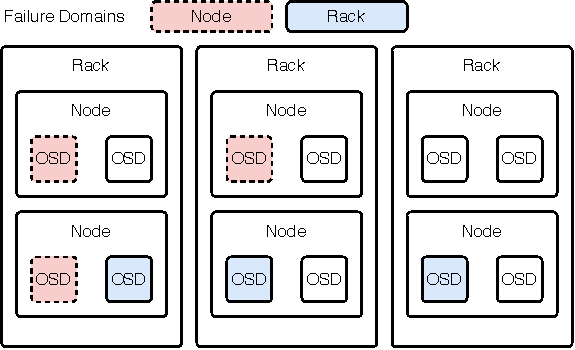
\includegraphics[width=0.5\linewidth]{assets/ceph/crush_failure_domains.pdf}
    \caption{CRUSH Failure Domains}
    \label{fig:crush-failure-domains}
\end{figure}

\Cref{fig:crush-failure-domains} demonstrates how this can be applied in
practice. For instance, for Ceph to protect against node failure resulting in
the loss of data, the placement rule's failure domain may be set at the node
level in the \ac{CRUSH} rule. In order to protect data against the failure of an
entire rack, the rule can be adapted accordingly and the placement is adjusted.
In this specific case, the object can withstand the loss of any two racks
without losing data. For \ac{HPC} specific use cases, it may be beneficial to
limit the replication in order to reduce latency. Placement rules may also
adjust the number of replicas (by default, this is three) or enable features
such as erasure coding.

Ceph also adds the \ac{PG} as an indirection layer for storage. Instead of
mapping an object directly to \acp{OSD}, the object is mapped to a \ac{PG}, and
the \acp{OSD} responsible for the \acp{PG} stores the \ac{PG} objects. This has
notable advantages over directly coupling objects to specific \acp{OSD}. The
main benefits are that recovery and balancing operations are greatly simplified.
Since object placement is tracked at the placement group level, determining the
data to be moved due to added or removed \acp{OSD} only requires knowing the
placement groups of the affected \ac{OSD}, of which there should typically not be more
than 100, according to Ceph recommended practices and defaults. The \ac{PG}
count can also remain static, even if the number of \acp{OSD} grows over time.

\subsubsection{\acs{CephFS}}

\ac{CephFS}---not to be confused with the Ceph storage system as a whole---is the file system support layer built on top of the existing Ceph \ac{RADOS} infrastructure. In effect, it acts as a translation layer between the hierarchical structure of a file system and the flat object storage that is Ceph's \ac{RADOS} layer. End users (in the context of this thesis, the users of the \ac{HPC} cluster) would simply see the file system without any changes needed to their workflows. In order to implement the file system, \ac{CephFS} relies on its \ac{MDS} daemons.

\subsubsection*{Metadata Servers}

\begin{figure}[htbp]
    \centering
    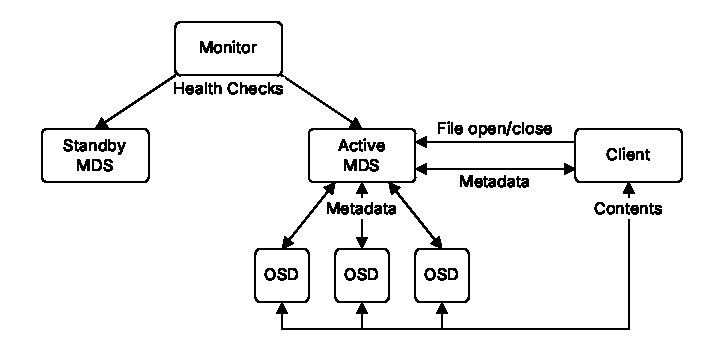
\includegraphics[width=0.9\textwidth]{assets/ceph/cephfs-mds-layout.pdf}
    \caption[CephFS Communication]
{Communication between Ceph \ac{MDS} daemons and clients as well as other Ceph
daemons in a CephFS setup. Clients request operations such as the
opening/closing of files from the \ac{MDS} and receive the appropriate metadata.
The contents of the files themselves are, however, written directly by the
client to the \acp{OSD}. Monitors perform health checking, instructing the
cluster to fail over to a standby \ac{MDS} in case the active \ac{MDS} fails.}
    \label{fig:cephfs-mds-layout}
\end{figure}

The \ac{MDS} is a core part of \acs{CephFS}. These daemons manage the state of the file system through synchronization with other \acs{MDS} daemons as well as acting as its source of truth for Ceph clients. However, for the actual file data itself, the client has access to the underlying \ac{RADOS} pool and can therefore communicate directly with \acp{OSD}, reducing the load on metadata servers. To achieve this, Ceph uses two separate pools for data and metadata, where the metadata may only be modified by \ac{MDS} daemons, and the data pool may be modified by Ceph clients directly. The metadata pool is also stored on top of \ac{RADOS}. The flow of operations is shown in \Cref{fig:cephfs-mds-layout}.

In order to improve metadata performance on slow pools, such as those backed by regular hard drives, the metadata pool may be on a separate storage class to that of the data pool. Since the metadata itself does not occupy as much space as the actual data, the metadata pool may be smaller than the bulk data pool. For instance, solid-state storage could be used. Common operations, such as a user listing their home directory, can then be served by this faster pool as well as the metadata cache of the \ac{MDS} itself.

\subsubsection*{Operating System Support}

On Linux, \ac{CephFS} supports three methods for accessing the Ceph file system: libcephfs, the \ac{FUSE} driver, and the kernel driver. The libcephfs library is a userspace library which allows applications to communicate directly with the Ceph cluster, i.e., with no mounting of the file system required. Of these three, the kernel driver is the most performant. However, it has the disadvantage of being bound to the kernel shipped with the distribution in use, unless a custom kernel is used.

\subsubsection{Comparison with Other File Systems}

Lustre shares some of the high-level design concepts with Ceph. Both cluster file systems are object stores at the lowest level, with a division of responsibilities between the management, storage, and metadata daemons, which can also be spread across multiple nodes~\cite[p.~308;pp.~6-9]{ceph-paper, lustre-manual}. However, the design philosophies of the two systems vary greatly.

Lustre, since its first full release, has historically been designed around achieving high performance and scalability for \ac{HPC} workloads\footnote{\url{https://lwn.net/Articles/63267/}. Dated 16.12.2003. Accessed 20.01.2026.}. In general, Lustre is not designed to provide redundancy for data, delegating this task to the lower level storage components, such as the underlying file system (e.g., ZFS) or a hardware \ac{RAID} controller. In this case, if a disk fails and is replaced, these lower-level components handle the necessary recovery steps. 

However, this does not provide failure tolerance in the case of node failure or other forms of hardware failure, such as cabling issues. In order for Lustre to be able to tolerate the failure of a single node, redundancy must be provided by external software. The recommended method for this is through the usage of Pacemaker and Corosync, which allows for failover of Lustre object storage servers~\cite{lustre-ha-wiki}, akin to a Ceph \ac{OSD} in terms of functionality. Nodes responsible for a specific \ac{OST} must both be connected to the storage (e.g., via an \ac{NVMeoF} connection to \acp{SSD}). This setup is shown in~\cref{fig:lustre-ha}. Without it, failure results in the data stored on that specific \ac{OST} becoming unreadable until the node is brought back up, and disk failure which cannot be corrected by the underlying storage system (e.g., 2-disk failure in a \acs{RAID}-5) results in the loss of all data on those disks.

\begin{figure}[htbp]
    \centering
    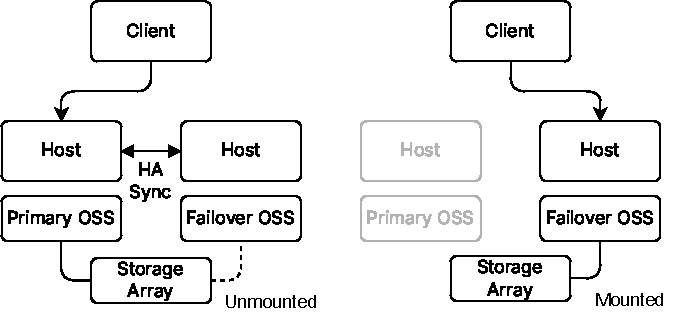
\includegraphics[width=0.75\linewidth]{assets/lustre/lustre_ha.pdf}
    \caption[Lustre \ac{HA} Concept]{High availability in the Lustre file system. Two nodes are connected to the same storage, with one node as the standby node. Upon failure of the primary node, the failover node takes over the task of serving the storage to clients. The Lustre architecture assumes that the underlying storage array is reliable, having a failover mode of its own.}
    \label{fig:lustre-ha}
\end{figure}

Versions of Lustre past 2.11.0, released in 2018\footnote{\url{https://www.lustre.org/lustre-2-11-0-released/}. Dated 03.04.2018. Accessed 20.01.2026.}, support a redundancy feature built into Lustre itself, known as \ac{FLR}. This feature allows for files to be replicated across multiple storage targets in a manner more similar to that of Ceph. However, the manual\footnote{\url{https://doc.lustre.org/lustre_manual.xhtml\#flr}. Accessed 20.01.2026.} describes this feature in more detail. Currently, this feature does not provide the strong guarantees that file systems such as ZFS or Ceph do---while writes are replicated to multiple object storage targets, they do not do so synchronously. A completed Lustre write on the client side with \ac{FLR}, therefore, does not guarantee that the desired replication level has been reached.

Overall, in its current revision, the underlying hardware must be highly reliable in order to be suitable for use within Lustre. However, possibly as a result of these assumptions, Lustre performs well as a \ac{HPC} file system~\cite{io500-full-list}. For instance, because no replication is used, the amount of network traffic can be reduced, increasing the amount of file \ac{I/O} operations possible within the bandwidth constraints.

\begin{figure}[htbp]
    \centering
    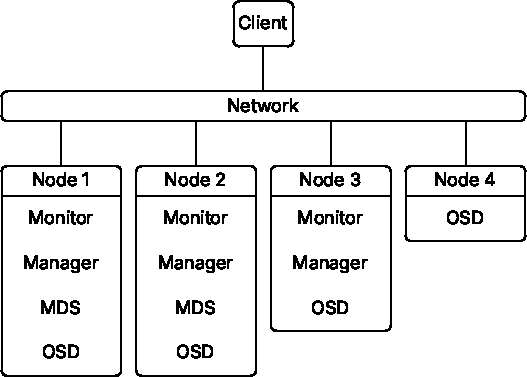
\includegraphics[width=0.5\linewidth]{assets/ceph/basic_ceph_cluster.pdf}
    \caption[Minimal Highly-Available Ceph Cluster]
    {
    The smallest highly-available Ceph cluster, containing the distribution of daemons necessary to allow for the continued functioning of the Ceph cluster after the failure of any one of the four nodes.
    }
    \label{fig:ceph-minimal-ha}
\end{figure}

Ceph, however, takes a much more conservative approach towards its expectations on hardware reliability~\cite{ceph-paper}, and is therefore much more flexible with its hardware requirements. While Lustre assumes the underlying hardware is reliable, Ceph assumes the hardware is unreliable and is therefore designed to handle failures on its own with its flexible \ac{CRUSH} algorithm, as detailed in~\cref{sec:ceph-crush}. This allows for the cluster to achieve its availability targets without highly-specialized hardware, potentially reducing costs. In~\cref{fig:ceph-minimal-ha}, a minimal highly-available cluster can be constructed with a small number of nodes, without \ac{RAID} on the \ac{OSD} backing storage. 

In summary, Lustre's approach to redundancy in the file system itself is explicitly opt-in, with none by default, while Ceph strongly discourages reducing redundancy. To opt out of redundancy in Ceph, it is not only necessary to enable the parameter mon\_allow\_pool\_size\_one, but to explicitly confirm intent when reducing pool sizes\footnote{\url{https://docs.ceph.com/en/latest/releases/pacific/}. Accessed 01.03.2026.}.



% Ceph, in this regard, is significantly more flexible with its hardware
% requirements. However, Lustre has historically performed well in
% \ac{HPC}~\cite{io500-full-list}, possibly as a result of these assumptions about
% the reliability of the underlying hardware. Network traffic, for instance, can
% be reduced significantly if no replication has to be performed.



% Due to the fact that Ceph is built with the presumption that nodes can and will
% fail, it performs its own health checks and maintains the redundancy level
% required by the user without the need for specific hardware or external
% software. This means, e.g., that instead of setting up a RAID-5 with 4 disks,
% the system administrator can instead assign one disk to one \ac{OSD} directly,
% and the required level of redundancy will be handled by Ceph according to the
% requirements (e.g., replica 3). This allows for the cluster to be highly
% available without requiring special hardware, which could potentially lower
% costs and increase reliability.




\medskip

\pagebreak
\section{Literature Review}
\label{sec:literature-review}

\subsection{Overview}

In this literature review section, we analyze the existing research surrounding Ceph, with a primary focus on its applications both within and outside of the \ac{HPC} contexts. We explore the existing literature on benchmarking methodologies as well as analyze historical Ceph performance results in order to provide context for the experimental results gathered in this thesis.

\subsection{Benchmarking}

The primary goal of this section is to determine a reference point for \ac{HPC} performance benchmarking, in order to establish a framework with which we can gather performance metrics using standardized tools. This framework will be applied to Ceph, allowing us to analyze results in a suitable context.

\subsubsection{Metric Selection}

By definition\footnote{\url{https://dictionary.cambridge.org/dictionary/english/benchmark}. Accessed 24.02.2026.}, benchmarks provide a common frame of reference within which
different systems or approaches can be compared. In the context of \ac{HPC},
this comparison is typically made based on metrics such as bandwidth, \ac{IOPS},
and latency, used to characterize the file system's performance under controlled
conditions.

While benchmarking tools can collect such
metrics\footnote{\url{https://github.com/hpc/ior}. Accessed 04.01.2026.},
interpreting these values can be challenging. The use cases for \ac{HPC} storage
are diverse, and whether a specific metric is relevant depends on the access
patterns of the workloads the cluster is realistically expected to process. In
addition, high performance in a single metric does not necessarily translate
into the file system being high performance in general.

In practice, the implementation of a file system requires trade-offs between
cost, capacity, throughput, and latency. \Cref{fig:storage-price-comparison}
demonstrates the differences between various storage media as well as system
memory\footnote{Price comparison data from \url{https://geizhals.de}. Consumer (PC) \acs{SSD}: WD SN7100, 4TB. Datacenter (DC) \acs{SSD}: Micron 7450
PRO, 3.84TB. \acs{HDD}: Seagate ST4000VN006, 4TB. \acs{DRAM}: Crucial CT2K64G56C46U5,
128GB. Accessed 12.01.2026.}. Note that currently, due to \acs{AI}-induced component shortages\footnote{\url{https://www.bloomberg.com/news/articles/2026-02-15/rampant-ai-demand-for-memory-is-fueling-a-growing-chip-crisis}. Accessed 24.02.2026.}, price data are highly unstable; however, the general comparison and price tiers remain valid at the time of writing.

\begin{figure}[htbp]
    \centering
    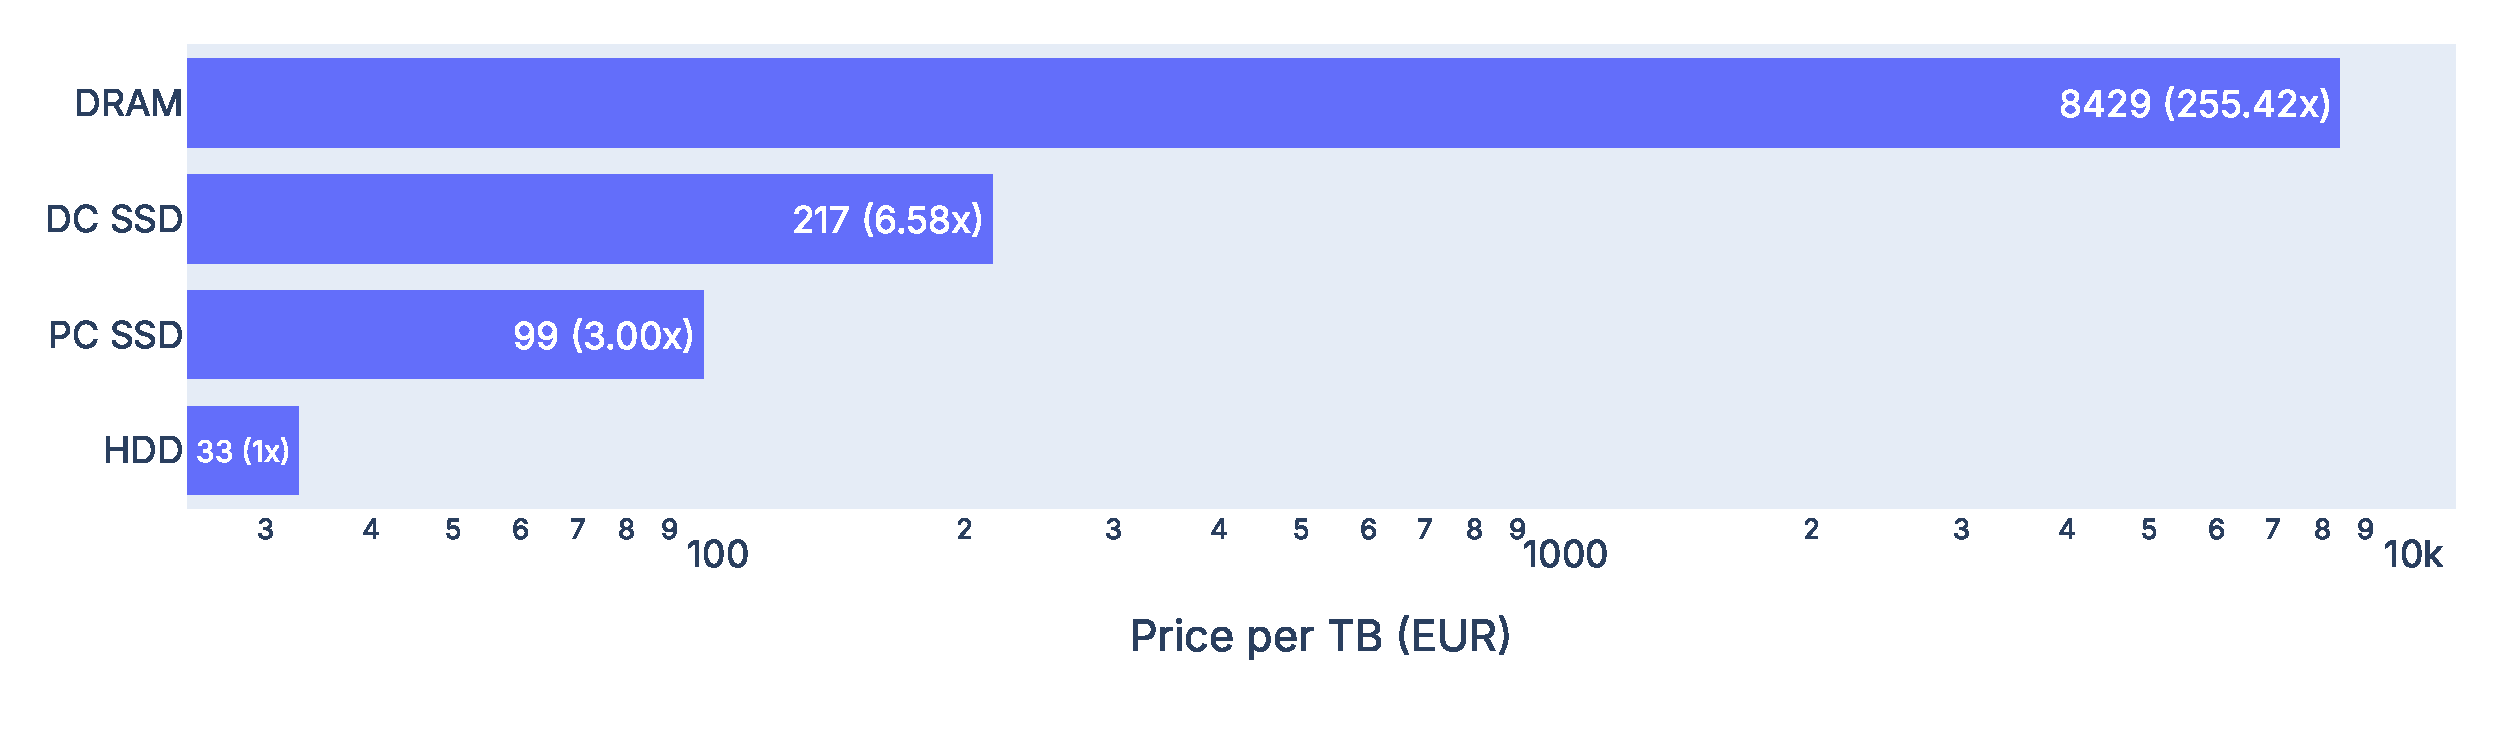
\includegraphics[width=\textwidth]{assets/charts/storage_price.pdf}
    \caption[Data Storage Price Comparison]{
    The normalized price (in Euros per terabyte) of selected storage media as well
    as \ac{DRAM}, as of 12.01.2026 (logarithmic scale) 
     }
    \label{fig:storage-price-comparison}
\end{figure}

In general, mechanical hard drives currently cost less than \acp{SSD} per
gigabyte of storage, while datacenter-grade \acp{SSD} can be significantly more
costly than standard \acp{SSD}. In this case, there is a direct trade-off
between performance and capacity, and not all workloads will necessarily benefit
from improvements to these characteristics. Real-world workloads could vary
significantly in the way that they access the file system---some workloads may
benefit from large, sequential file access, while others could be more random in
nature (see \Cref{sec:access-patterns}). Furthermore, there could be use
cases benefitting purely from capacity over other factors.

Determining which metrics are important for the workloads users will run
can therefore be difficult. However, there exist standardized benchmarks for 
\ac{HPC} storage systems, which aim to cover a wide range of access patterns 
and file sizes, with the goal of providing the best and worst case performance
results for comparison with other systems.

\subsubsection{Benchmarking Tools}
\label{sec:benchmarking-tools}

\ac{IOR} is a storage performance benchmarking tool initially developed at the
\ac{LLNL} in the early 2000s to test the \ac{I/O} performance of the
storage system used in their \ac{HPC}
cluster\footnote{\url{https://web.archive.org/web/20021110104515/https://www.llnl.gov/asci/purple/benchmarks/limited/ior/}.
Archived from the original page, dated 19.09.2001. Accessed 12.01.2026.}. Since
its original implementation, \ac{IOR} remains in active use for the evaluation of
file system performance in \ac{HPC}, with additional features and storage backends
supported\footnote{\url{https://github.com/hpc/ior}. Accessed 24.02.2026.}. Unlike many traditional
benchmarking tools, \ac{IOR} allows for clients running the benchmark to communicate
between each other in order to synchronize their operations and run in parallel.
This feature has the benefit of potentially producing more accurate results, as
well as more closely mimicking the behaviour of \ac{HPC} workloads, which can be
distributed among a large number of nodes. These nodes compete for access to the
same shared storage (e.g., a file system containing datasets for distributed
analysis), which can place a uniquely stressful load on such storage systems.

The mdtest benchmark, included as part of the \ac{IOR} repository, uses the same storage interfaces as the \ac{IOR} benchmarks. However, it is intended to test the metadata performance of \ac{HPC} file systems. Metadata, in this context, refers to the ancillary data stored alongside the contents of the files themselves, such as file names, attributes, folders, and storage locations. To that end, it supports the benchmarking of various operations, such as opening and closing files and directories and stat operations, used for reading attributes such as file size.

IO500\footnote{\url{https://github.com/io500/io500}. Accessed 24.02.2026.} is a standardized storage performance benchmark suite combining the \ac{IOR}
and mdtest benchmarks as well as runs of the find tool, the latter of which is
used to evaluate the performance of file searches. Instead of targeting a
specific use case, it provides a composite score, as well as sub-scores for
different performance profiles, such as ``easy'' \ac{IOR} performance (sequential
reads of a comparatively small number of large files) and ``hard'' mdtest
performance (large numbers of file operations). This establishes a bounding box
for storage performance by providing both worst-case and best-case bandwidth and
metadata results. These results can be compared with the access patterns of
production workloads in order to form a rough prediction of the expected range
in which the workload is expected to perform, given the benchmark results.
Naturally, this raises the question of which access patterns production
\ac{HPC} workloads typically exhibit.

\subsection{\acs{HPC} \acs{I/O} Access Patterns}
\label{sec:access-patterns}

Shan et al.~\cite{hpc-io-prediction} characterize the \ac{I/O} access patterns of traditional \ac{HPC} applications as primarily sequential, although the access sizes may vary by workload. The authors describe two write patterns:

\begin{itemize}
    \item The per-task (N-to-N) pattern, where each process writes its results to its own independent file
    \item The single-shared-file pattern, where each process writes its results to a block within a single shared output file
\end{itemize}

In both of these patterns, the authors observed that individual tasks write their results sequentially to the file system. Their model using the \ac{IOR} benchmark predicted the performance of these workloads well, with a prediction error of under 10\%. We therefore consider \ac{IOR} a valid proxy for the \ac{I/O} access patterns of these traditional \ac{HPC} applications.

However, the \ac{HPC} landscape has shifted significantly since the release of this 2008 report. In particular, the popularity of \ac{AI}, \ac{ML}, and data analytics workloads has increased rapidly. A recent survey by Lewis et al.~\cite{lewis_io_2025} characterizes the access patterns of these modern applications, demonstrating an access pattern considerably different from those of older \ac{HPC} workloads. In particular, \ac{ML} training workflows, particularly those utilizing methods such as \ac{MBGD}, are characterized by frequent random read accesses to relatively small files. These file operations generate heavy metadata accesses, potentially overwhelming the \ac{MDS} services of parallel file systems such as the surveyed Lustre file system, resulting in bottlenecks to training performance~\cite[p.~18]{lewis_io_2025}.

Beyond the primary \ac{HPC} workloads previously discussed, \ac{HPC} file systems can also be used to support ancillary tasks. While workloads such as software compilation, Git operations, and various other operations in users' home or project directories are less bandwidth-intensive than those of the aforementioned primary workloads, they are often dominated by metadata accesses and involve high numbers of file open, close, stat, and create operations on small files. For example, initializing a standard Python virtual environment without the installation of any additional dependencies creates approximately 1700 small files\footnote{Tested on Python 3.11.9}, and cloning a large Git repository such as that of Ceph's latest release branch\footnote{Git clone of \url{https://github.com/ceph/ceph}, \texttt{tentacle} branch. Accessed 26.02.2026.} creates a directory containing several subdirectories with a total of 19,000 small source and metadata files, with each file ranging from a few kilobytes to megabytes in size.

The performance degradation of such workloads for the performance of networked file systems has been documented. Krotkiewski~\cite{Krotkiewski_2017} demonstrated that small-file operations on the BeeGFS parallel file system incur significant performance penalties due to the overhead and latency introduced by metadata operations. To mitigate this issue, the study stored data within disk images formatted with a regular file system (ext4), which resided on the parallel file system and were mounted locally as loopback devices. This results in metadata operations within the loopback device being performed locally, significantly reducing the load on the parallel file system's metadata servers. This approach significantly improved the performance of metadata-intensive tasks, such as searching for files, deleting complex directory trees, and software compilation, reducing their overall time to complete.

\begin{figure}[htbp]
    \centering
    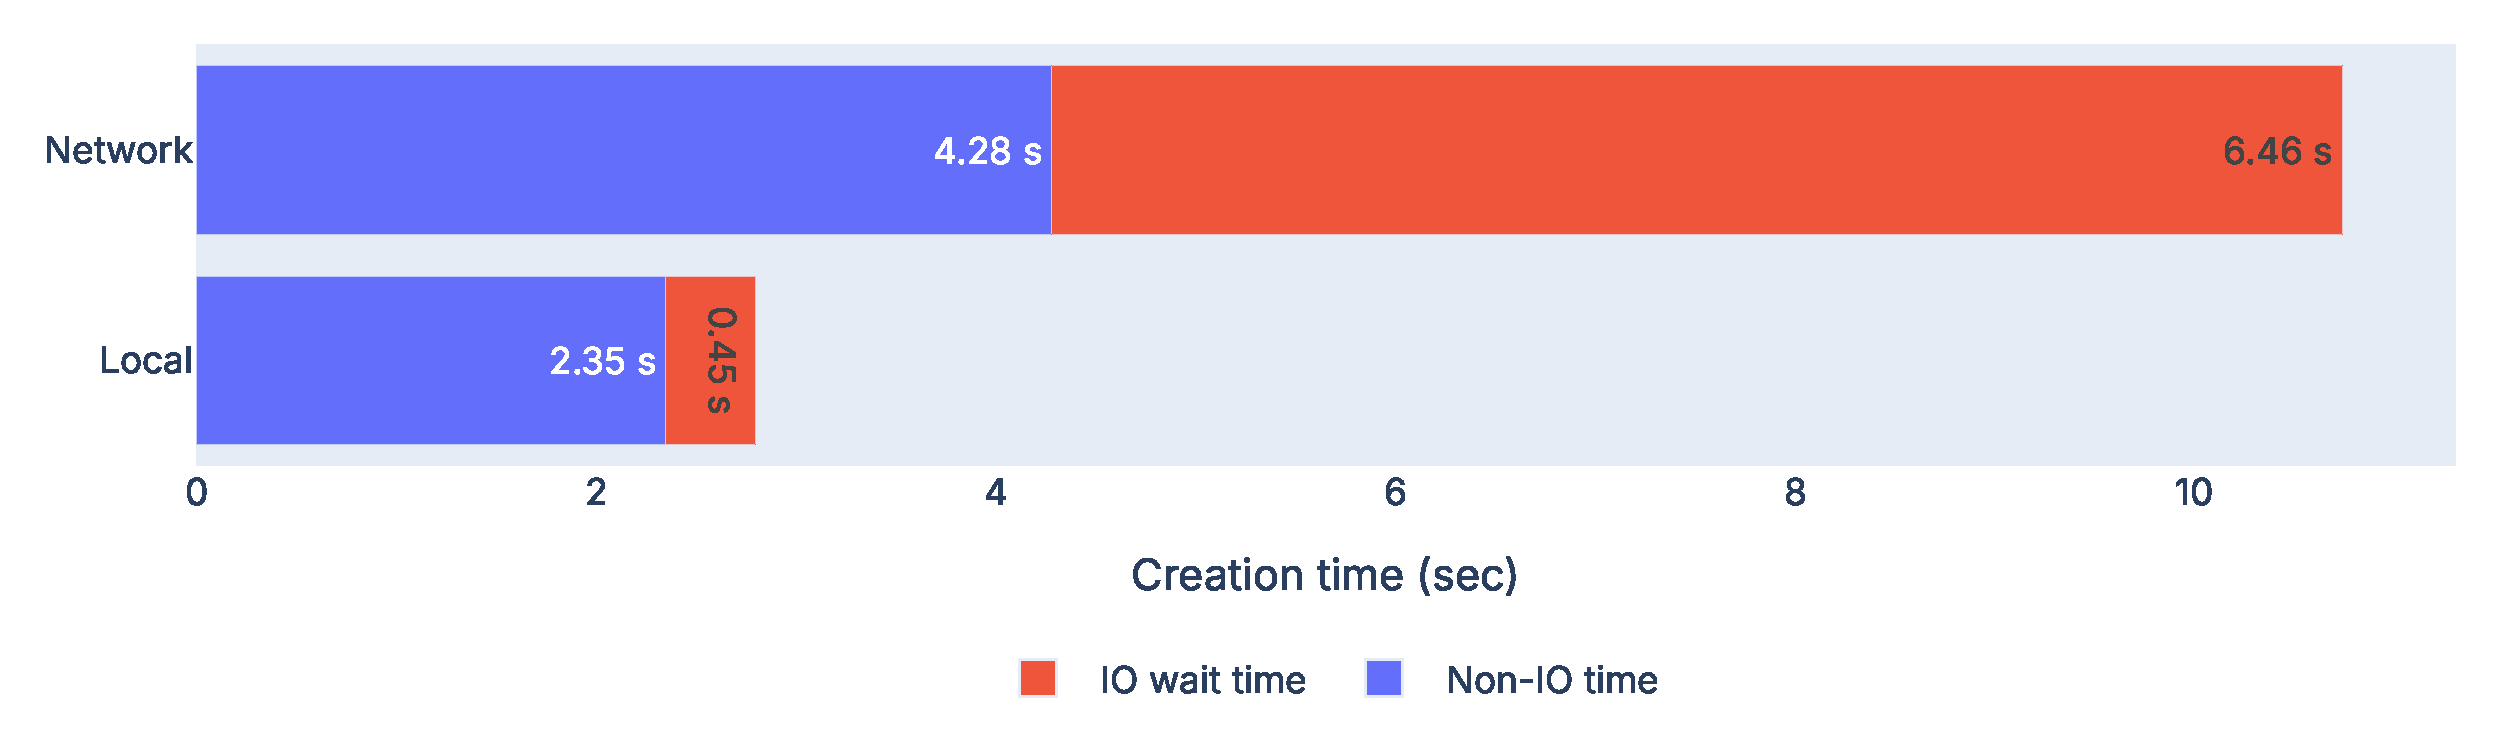
\includegraphics[width=\textwidth]{assets/charts/venv_creation_time.pdf}
    \caption[Python virtual environment creation time]
    {
    Time in seconds required to create a Python virtual environment, with non-\ac{I/O} (user) time and \ac{I/O} wait time shown. When running over a network file system, overall execution time increases significantly, and \ac{I/O} wait time makes up a significant portion of the total time required.
    }
    \label{fig:python-venv-create-time}
\end{figure}

Testing on the production home file system of the \ac{GWDG} \ac{HPC} cluster produces similar results. \Cref{fig:python-venv-create-time} demonstrates the performance impact of the creation of a Python virtual environment on a local tmpfs file system in comparison to a \ac{HPC} file system (in this case, Vast). The creation time of the virtual environment was 3.8$\times$ higher, while the \ac{I/O} wait time increased by over 14$\times$. In total, the 1700 created files had a comparatively small disk utilization of 25 MB, resulting in an effective throughput of 2.35 MB/s, several orders of magnitude lower than the theoretically achievable performance of both the network and storage systems when handling sequential \ac{I/O} operations: for example, creating a 32GB test file using \texttt{dd} resulted in a \acs{CPU}-limited throughput of 1 GB/s, or a throughput roughly 400$\times$ greater than that of the Python virtual environment workload.

As a result, we also consider evaluating Ceph's metadata performance as crucial for determining its viability in \ac{HPC}. This applies not only to modern \ac{AI}/\ac{ML} applications, but also as a general-purpose storage backend for \ac{HPC} home and scratch directories.

\subsection{Ceph Architectural Changes}
\label{sec:ceph-architecture}

The basic architectural concepts within Ceph discussed in \Cref{sec:background} have remained largely stable since the project's inception. However, the implementations of these concepts have evolved significantly over time. One of the most relevant changes are the backends Ceph uses to store data on storage devices~\cite{filesystems-unfit-bluestore}.

Early versions of Ceph relied on the FileStore backend, in which \ac{OSD} data were stored on a traditional file system, generally XFS\footnote{\url{https://docs.ceph.com/en/mimic/man/8/ceph-deploy}. Accessed 24.02.2026.}. While this approach abstracted much of the complexity of storing data on the disk away, it introduced notable performance limitations. In particular, transactional and metadata operations incurred significant overheads. As storage hardware evolved, especially with the growing adoption of fast \ac{NVMe} \acp{SSD}, these limitations became increasingly pronounced, constraining Ceph's scalability and motivating the development of a new storage backend known as BlueStore in 2016. The backend removes the dependency on a traditional file system by communicating with disks directly, as well as integrating journaling directly into the backend itself. This redesign significantly reduced overhead, with initial versions showing substantial improvements of up to 80\% for operations such as object creation~\cite[p.~358]{filesystems-unfit-bluestore}. BlueStore became stable and the default backend in 2017. As of 2023 in the Ceph Reef release, FileStore was removed as a backend entirely\footnote{\url{https://docs.ceph.com/en/reef/ceph-volume/lvm/prepare/\#filestore}. Accessed 24.02.2026.}.

However, advancements in high-performance \ac{NVMe} \acp{SSD} have motivated the development of a new backend known as SeaStore\footnote{\url{https://docs.ceph.com/en/tentacle/dev/seastore/}. Accessed 06.01.2026.}. This implementation is specifically designed to take advantage of high-performance \acp{SSD}. At the time of writing, SeaStore remains an experimental feature under heavy development, and as a result comprehensive performance evaluations are not yet available. Nevertheless, it is likely that future Ceph releases will see SeaStore becoming the standard backend for high-performance \ac{NVMe} \ac{SSD} storage, potentially improving Ceph's performance further.

Therefore, while Ceph is considered a stable and mature platform, it continues to undergo significant changes to its architecture. This history and ongoing development should be considered when reviewing historical performance results for Ceph, especially those using the FileStore backend, as they may no longer be relevant for modern Ceph versions.

\subsection{Ceph Performance}

Although Ceph has existed in some capacity since 2006, uptake in the \ac{HPC} field has been limited. Ceph has seen successful deployments for cloud computing purposes with frameworks such as Rook\footnote{\url{https://rook.io/}. Accessed 26.02.2026.}, as well as for high-reliability data storage in businesses, where the requirements may differ from those of \ac{HPC} workloads. Nevertheless, there have been a few benchmarks of the Ceph file system specifically for \ac{HPC} workloads.

\subsubsection{Early Performance Testing}

One of the earliest performance evaluations of Ceph in an \ac{HPC} context was
performed in 2013 at the \ac{ORNL}~\cite{ceph-ornl-evaluation-filestore}, a
research laboratory which at the time primarily used Lustre for storage of its
data.

The test platform utilized arrays of \ac{SATA} and \ac{SAS} based \acp{HDD} in a \ac{RAID} 6 configuration on top of the FileStore backend.  These benchmarks demonstrated a performance of about 70\% of the raw hardware capabilities. However, due to the design of the FileStore backend---most notably the journaling method---effective write throughput was reduced to half the raw write performance due to the need to initially write data to the journal, followed by backing storage. Despite these limitations, and considering the early state of the Ceph file system at the time, the authors described the tuned performance as satisfactory. 

That being said, the study highlighted one of the largest weaknesses of the Ceph file system at the time, namely journaling overhead of the FileStore backend. The introduction of the BlueStore backend, which substantially altered the way Ceph interacts with disks as described in \Cref{sec:ceph-architecture}, would likely have mitigated some of the issues demonstrated in the paper. However, this paper is still relevant for our analysis as it demonstrates the significant changes and performance improvements Ceph has undergone since its early versions.

\subsubsection{Modern Performance Tests}

More recent evaluations have been performed after Ceph's switch to BlueStore. A study by CERN evaluated Ceph as a data backend for their custom-developed \ac{EOS} system~\cite{cern-evaluating-cephfs-perf}, used for the storage of experiment data (most notably, data gathered as part of particle accelerator experiments). According to the paper, CERN already deploys \ac{CephFS} as \ac{HPC} scratch storage, in addition to other general-purpose use cases. However, limitations such as limited authentication mechanisms and external interfaces---for instance, via HTTP-based access---and the absence of high-throughput testing have limited the application of Ceph to other storage use cases within CERN.

% \cite[p.~2]{cern-evaluating-cephfs-perf}

In the evaluated configuration, \ac{CephFS} was deployed on top of \acs{HDD}-based \acp{OSD} for data storage, with \acp{SSD} being used to store metadata for the \ac{MDS} daemons. Rather than using Ceph's default replica-3 strategy, the system was deployed with erasure coding with a \acs{RAID}-6-like erasure coding configuration from 4 data + 2 coding chunks for 2-disk failure tolerance, to 16 data + 2 coding chunks.

% \cite[pp.~2--3]{cern-evaluating-cephfs-perf}

The results indicate that the per-stream throughput was relatively low with  <400\,MB/s reads and <430\ MB/s writes for a single client. However, aggregate throughput with multiple clients scaled well. Individual nodes were capable of 4.5/5.9 GiB/s of read/write throughput, while the total read/write throughput scaled to 22/34.3 GiB/s~\cite[p.~4]{cern-evaluating-cephfs-perf}. The write performance was deemed to be close to the network limit, while the read performance was likely bottlenecked not by Ceph, but the hard disks themselves.

% \cite[p.~4]{cern-evaluating-cephfs-perf}

Certain issues with Ceph were also reported. A single \ac{OSD} had a disproportionate impact on the overall throughput, dropping write throughput by 80\%. In addition, the default tunable parameters lead to suboptimal performance due to \ac{I/O} stalls at high bandwidths. There was also an issue with \acp{MDS} potentially running out of memory due to the heavy metadata loads \ac{EOS} placed on the file system, however, this was patched in their evaluation and has since been accepted into upstream Ceph\footnote{\url{https://github.com/ceph/ceph/pull/38574}. Accessed 04.01.2026.}.

% \cite[pp.~6--7]{cern-evaluating-cephfs-perf}

While not a peer-reviewed publication, the highest-performing publicly available performance results for Ceph were achieved by Clyso for an unnamed customer in 2023, where they achieved 1\,TiB/s of peak performance for a large-scale Ceph deployment backed by \ac{SSD} storage~\cite{ceph-1tib}. The report details a 63-node cluster consisting of 630 \acp{SSD} in total, with 10 \acp{SSD} and dual 100 Gigabit Ethernet networking per node. The report demonstrated very high aggregate performance with up to 1025/270\,GiB/s of read/write throughput using replication and 547/387\,GiB/s using erasure coding. Additionally, they identified issues with per-node \ac{IOPS} limitations, where each individual node could not exceed 400--600K \ac{IOPS} due to Ceph's messenger implementation, and identified this as a potential source of improvement. However, these performance results were not gathered with \ac{CephFS}, rather with the lower-level \ac{RBD} block storage interface.
\subsection*{Summary}

Existing literature illustrates that while the landscape for \ac{HPC} workloads has shifted significantly over time, their access patterns can still be accurately modeled by existing \ac{HPC} storage performance benchmarking tools: large sequential read behaviour of traditional \ac{HPC} applications can be emulated accurately by \ac{IOR}, while small-file-\acs{I/O} and other metadata-heavy operations in \ac{AI}/\ac{ML} can be modeled by mdtest. Ancillary workloads, such as common operations performed by users interactively on their home directories are similarly metadata-heavy, and are likewise modelable using mdtest. Benchmarking suites such as the IO500 leverage both tools in order to establish a bounding box for file system performance, capturing both best and worst-case performance metrics for both data throughput and metadata operations.

In addition, Ceph has evolved significantly from its early versions. In particular, the transition from FileStore to BlueStore for \ac{OSD} backing storage resolved many of Ceph's major performance bottlenecks, and has allowed Ceph to more effectively utilize modern technologies such as \ac{NVMe} flash storage. However, while reports have shown high aggregate throughput results, per-client performance may be constrained by communication overhead, possibly exacerbated by the \ac{CPU} overhead of the \ac{TCP/IP} networking stack on which Ceph relies. Furthermore, the compounding factor of underlying physical disk performance, particularly with \acs{HDD}-backed \acp{OSD}, obscure some of the intrinsic architectural limitations of Ceph's software stack. 

Given that Ceph is significantly more reliant on its software logic than incumbent solutions such as Lustre, it is necessary to decouple the limitations of the hardware from the storage system itself. Therefore, our methodology employs memory-backed storage to mitigate storage performance as a compounding factor, allowing us to directly stress and analyze the performance of Ceph's abstraction layers---in particular that of \ac{RADOS} and \ac{CephFS}.


% !TEX root = main.tex

\pagebreak
\section{Methodology}
\label{sec:methodology}

In this section, we detail the experimental methodology designed to evaluate the Ceph file system for \ac{HPC} environments. A specialized approach was necessary due to the unique requirements and constraints of \ac{HPC} environments. These include factors such as the lack of root privileges on standard \ac{HPC} compute nodes, dynamic allocation of compute resources, as well as our requirement to isolate hardware performance. Consequently, the primary goals of the methodology detailed in this section are as follows:

\begin{itemize}
    \item To engineer an automated deployment framework capable of rootless provisioning of Ceph clusters, integrating with standard \ac{HPC} cluster nodes, workload managers such as Slurm, and rootless \acs{HPC}-optimized container runtimes, such as Apptainer.
    \item To eliminate bandwidth and latency limitations of physical hard disks from performance measurements through the use of Ceph's memory backed storage backend, allowing for our evaluation to focus on Ceph's internal abstraction layers.
    \item To establish a tuned baseline for network communication performance over common \ac{HPC} fabrics---specifically, the Omni-Path and InfiniBand fabrics available on the \acs{GWDG} cluster---in order to potentially attribute possible performance bottlenecks which arise to Ceph's reliance on the \ac{TCP/IP} stack for its communication.
    \item To construct a performance testing pipeline using \ac{HPC} \acs{I/O} performance benchmarking tools such as \ac{IOR} and mdtest, which test multiple \ac{I/O} access patterns common in \ac{HPC} at various scaling levels.
    \item To establish a secondary Ceph cluster with tightly-controlled performance parameters, in order to evaluate the system administration and theoretical performance scaling aspects of the file system.
\end{itemize}

The subsections which follow describe our evaluation of existing cluster deployment tools, our custom Ceph deployment system, network tuning, and our benchmarking framework.

\subsection{Deployment Tools}

Ceph clusters can be deployed using a variety of standard tools. However,
several challenges were presented when attempting to implement these in the
\ac{HPC} test environments that were available for this thesis. We will
initially cover existing tools for production deployments, followed by the
deployment tool created for this thesis.

\subsubsection{Cephadm}
\label{sec:cephadm}

Cephadm is a first-party orchestration tool designed for the deployment of Ceph clusters. It manages cluster deployment by performing setup operations such as storage provisioning and placement of daemons on participating cluster nodes. It is generally the recommended tool for the deployment of production-ready Ceph clusters\footnote{\url{https://docs.ceph.com/en/latest/install/}. Accessed 21.01.2026.}.

The Cephadm orchestrator requires root permissions in order to perform operations such as storage configuration, as well as an interface to either Docker or Podman as a container runtime, used to create daemon containers. The hardware available for this thesis, standard \ac{HPC} cluster nodes, neither allowed for root access nor access to a fully-featured Podman or Docker installation. Instead, only the Apptainer container runtime was provided.

In addition, modern Ceph versions use the BlueStore storage backend, which performs read/write operations directly on block devices (i.e., physical disks, partitions, or logical volumes) rather than using an intermediate file system. This requires both the hardware (i.e., the disks themselves to be available), as well as the permissions necessary to read and write to them. Both of these options were not available on the \ac{HPC} cluster. While the legacy FileStore backend could have theoretically been run rootless, we do not consider the data gathered from this backend to be useful for evaluation. This is primarily due to the fact that, since January 2025, the last Ceph version with support for the FileStore Backend (17, Quincy) is unsupported\footnote{\url{https://docs.ceph.com/en/latest/releases/\#active-releases}. Accessed 02.02.2026.}.

The cephadm utility will still be used in this thesis to evaluate the
system administration aspect of the file system. However, because the hardware available for this purpose consists of a single performance- and network-limited computer, large-scale stress testing will not be performed on the Cephadm-deployed cluster. This deployment is referred to as the
\enquote{Production Deployment} and detailed further in~\cref{sec:production-deployment}.

\subsubsection{Alternatives}

Other orchestration tools, such as Rook, have similar requirements which complicate deployment on the \ac{HPC} cluster. Due to the aforementioned permission limitations and the desire to eliminate sources of variance outside of Ceph's direct control as much as possible, such as variations in \ac{SSD} performance, a custom deployment and benchmarking method was implemented in this thesis.

\subsection{Custom Deployment}
\label{sec:custom-deployment}

Due to the unique limitations of the cluster, as well as the time-consuming and therefore impractical nature of deploying several different cluster configurations manually, a custom deployment tool was created in this thesis in order to deploy and benchmark Ceph clusters of various sizes as well as under various client workloads. The tool has been named \enquote{Cuttlefish} and will be referred to as such in the following sections.

Cuttlefish is built for Ceph cluster deployment taking into account the limitations of the \ac{HPC} cluster. Specifically, it must function under the following constraints:

\begin{itemize}
    \item Elevated privileges are not required on any node in the cluster.
    \item Daemons must run either without a container engine, or on Apptainer, the latter of which was available on the test nodes.
    \item The number of daemons of each type as well as the distribution should be configurable.
    \item The orchestrator should be capable of deploying daemons on dynamically allocated nodes, which have varying \ac{IP} addresses and may not be pre-configured.
\end{itemize}

Cuttlefish is built to work with Apptainer and Slurm. Slurm is used for the allocation of nodes from the \ac{HPC} cluster pool, and Apptainer is used to run the daemons in containers regardless of the host operating system. The latter is similar to the method used by Cephadm, although the container runtime is different.

Due to the BlueStore backend's reliance on direct disk access, it is not possible to run large-scale BlueStore tests on the \ac{HPC} cluster without root permissions. However, Ceph provides a memory-backed storage backend. This backend, known as MemStore, is designed primarily for testing purposes, and does not require elevated privileges---objects are stored in \ac{RAM}. For the purposes of these benchmarks, this backend is sufficient, as the goal of our benchmarking process is to identify bottlenecks within Ceph itself, rather than the limitations of the underlying disks. Being an in-memory storage backend, MemStore is less likely to be a bottleneck due to the higher bandwidth and lower latency provided by \ac{RAM}. Given that the memory bandwidth is significantly higher than the network bandwidth, we assume that the network becomes a performance bottleneck before memory does. To validate this, prior to running benchmarks, the memory bandwidth of the system will be tested using the Intel Memory Latency Checker\footnote{\url{https://www.intel.com/content/www/us/en/download/736633/intel-memory-latency-checker-intel-mlc.html}. Accessed 26.02.2026.} (mlc), or pmbw\footnote{\url{https://panthema.net/2013/pmbw/}. Accessed 26.02.2026.} if mlc is not capable of running due to system constraints.

A summary of the communication between the various involved systems is summarized in \Cref{fig:cuttlefish_deployment_seq_diagram} as a sequence diagram. Additionally, we will use an example cluster to demonstrate how the system state is modified by the various steps in the deployment process, shown in~\cref{tab:example-cluster-layout}.

\begin{table}[h]
    \centering
    \begin{tabular}{|ccccccc|}
        \hline
        Hostname & IP Address & \acs{RAM} & Monitors & Managers & \acp{MDS} & \acp{OSD} \\
        \hline
        node1    & 192.0.2.1 & \multirow{4}{*}{256 GiB} & 1        & 1        & 1         & ---       \\
        node2    & 192.0.2.2 & & ---      & ---      & ---       & 3         \\
        node3    & 192.0.2.3 & & ---      & ---      & ---       & 4         \\
        node4    & 192.0.2.4 & & ---      & ---      & ---       & 3         \\
        \hline
    \end{tabular}
    \caption[Example Cluster Layout]{An example cluster layout which will be used for demonstration purposes.}
    \label{tab:example-cluster-layout}
\end{table}

\begin{figure}[htbp]
    \centering
    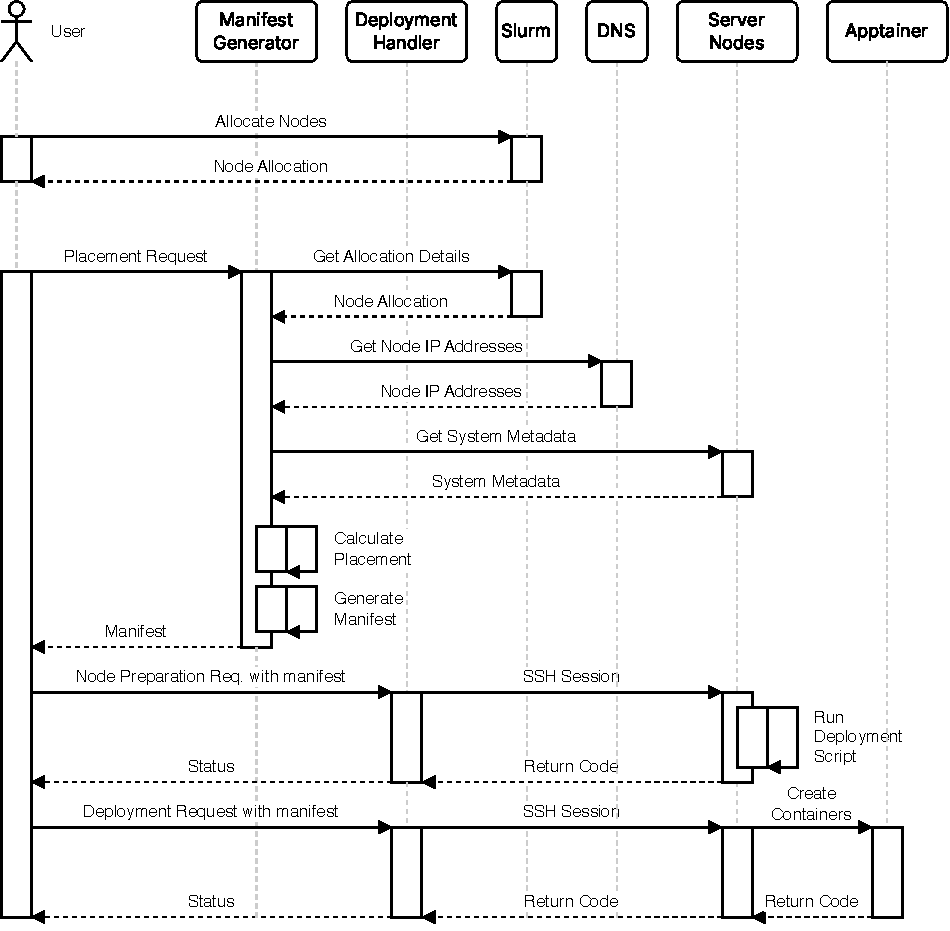
\includegraphics[width=\linewidth]{assets/cuttlefish/deployment_seq_diagram.pdf}
    \caption[Cluster deployment sequence diagram]{
Sequence diagram for the cluster deployment process. The deployment scripts
(manifest generator and deployment handler) communicate with external services
in order to generate a manifest containing all necessary details to start the
cluster. With the complete manifest, the deployment handler communicates with
participating nodes and their container runtimes to bring up the requested
daemons.
}
    \label{fig:cuttlefish_deployment_seq_diagram}
\end{figure}

\subsubsection{One-Time Operations}

Certain operations within the deployment must only be performed once and can be reused across an unlimited number of cluster deployment and teardown cycles.

Ceph daemons and clients communicate with each other using an encrypted protocol known as cephx\footnote{\url{https://docs.ceph.com/en/tentacle/dev/cephx/}. Accessed 20.01.2026.}. Monitor nodes contain the keys of all nodes, including their own key shared across the monitors, while individual daemon types only have their own keys. The keyring then contains the keys as well as the allowed permissions: an example of a keyring file can be found in~\cref{appendix:sample-ceph-keyring}.

Access to a Ceph cluster is not required for this step, only the command line tools which are available in the upstream Ceph container image. Cuttlefish includes a tool which generates this keyring file once, with configurable permissions. This keyring file is then used and preserved across different deployments and reconfigurations. For example, the keyring can contain keys for 512 \acp{OSD} and 10 monitors, even if the deployed cluster never contains this many daemons. The rest of the keys in the keyring are simply ignored until more daemons are created.

\subsubsection{Node Allocation \& Placement}
\label{sec:node-allocation-placement}

The nodes available for testing during this thesis were part of the regular production compute cluster at the \ac{GWDG}. Nodes are allocated on-demand, and change depending on node availability. Therefore, a request to allocate e.g., 16 nodes on a cluster may return a different set of nodes depending on the nodes used by other users' jobs. A job was first allocated using the \texttt{salloc} command, which creates a node allocation for the cluster deployment system to use. \Cref{lst:slurmalloc} shows a typical distribution of nodes after an allocation is granted, gathered using \texttt{squeue}\footnote{Output from \texttt{squeue -{}-me} formatted to remove unnecessary/internal information.}.

\lstinputlisting[
    caption={
        [Slurm Node Allocation]
        A typical Slurm node allocation performed on the \ac{GWDG} compute cluster's 
        \texttt{medium96s} partition, containing a set of nodes ready for use.
    },
    label={lst:slurmalloc},
    frame=single,
    breaklines=true
]{assets/cluster/squeue-me.txt}

Due to the dynamic nature of the allocations, we automate the mapping of Ceph daemons onto nodes. The user may specify the desired state of the cluster at a high level, and the placement will be performed according to the user's instructions. The placement algorithm allows for the following requirements and constraints to be taken into consideration:

\begin{itemize}
    \item Total number and type of daemons (e.g., 1 monitor, 1 \ac{MDS}, 8 \acp{OSD})
    \item Number of nodes to use from the Slurm allocation
    \item Adjustment of constraints per daemon type
    \begin{itemize}
        \item Density: the maximum number of daemons of this type to place on a node
        \item Allowed overlaps: if no free nodes are available, allow placement on an already occupied node
        \item Disallowed overlaps: do not allow the co-location of this daemon on a node with specific daemon types (e.g., monitor and \ac{OSD} must not overlap)
        \item Required overlaps: require that the daemon be placed with another daemon of the specified type
    \end{itemize}
    \item Placement type
    \begin{itemize}
        \item Spread (S): Place daemons on the least loaded nodes
        \item Group (G): Group daemons on the most loaded node up to the density limit before considering other nodes
    \end{itemize}
\end{itemize}

The default placement policy is shown in~\cref{tbl:allowed-daemon-overlaps}.

\newcommand{\YesMark}{%
  \tikz\fill (0,0) rectangle (1.2ex,1.2ex);%
}
\newcommand{\NoMark}{%
  \tikz\draw (0,0) rectangle (1.2ex,1.2ex);%
}
\newcommand{\RequiredMark}{%
  \tikz\fill
    (0,0) --
    (1.2ex,0) --
    (0.6ex,1.2ex) --
    cycle;%
}

\begin{table}[h]
    \begin{center}
        \begin{tabular}{|cc|lcccc|}
            \hline
            \rotatebox{90}{Placement~} & \rotatebox{90}{Density~} & & \rotatebox{90}{Monitor~} & \rotatebox{90}{Manager~} & \rotatebox{90}{\acs{MDS}~} & \rotatebox{90}{\acs{OSD}~} \\
            \hline
            Spread & 1 & Monitor & \NoMark  & \YesMark & \YesMark & \NoMark \\
            Spread & 1 & Manager & \RequiredMark & \NoMark  & \YesMark & \NoMark  \\
            Spread & 128 & \acs{MDS} & \YesMark & \YesMark & \YesMark & \NoMark \\
            Spread & 128 & \acs{OSD} & \NoMark  & \NoMark  & \NoMark  & \YesMark \\
            \hline
        \end{tabular}
    \end{center}
    \begin{center}
        \begin{tabular}{ccccccc}
             Overlaps: & \NoMark & Disallowed & \YesMark & Allowed & \RequiredMark & Required \\
        \end{tabular}
    \end{center}
    \caption[Default Placement Policy]{The default daemon placement policy. The daemon types on the left represent the daemon to be placed, and the daemon types in the table header represent the existing daemons on the node.}
    \label{tbl:allowed-daemon-overlaps}
\end{table}

\subsubsection{Ceph Autoconfiguration}
\label{sec:ceph-autoconfig}

The template Ceph configuration is similar to that of a regular Ceph cluster: it contains the startup configuration shared across all nodes. However, in addition to the template itself, additional fields are added to the final configuration in order to allow for the cluster layout to change while keeping the template configuration static. \Cref{lst:ceph-conf} shows an example of a minimal ceph.conf which contains a configuration for a Ceph cluster with MemStore \acp{OSD}.

\lstinputlisting[
    language=ini,
    caption={
    [Minimal Ceph Configuration]
    Minimal configuration file used for bootstrapping the Ceph cluster, allowing for
    options to be changed by the user manually prior to the bring-up of the cluster.
    For instance, the default minimum pool size is reduced to 1 for testing purposes.
    },
    label={lst:ceph-conf},
    frame=single,
    breaklines=true
]{assets/cuttlefish/example.ceph.conf}

Ceph daemons require the location of monitor nodes to be defined in the configuration. Instead of being hardcoded into the configuration, the monitor node list is generated dynamically based on the node allocation and placement policy as described in~\cref{sec:node-allocation-placement}. Once daemons have been allocated to nodes, the \ac{IP} addresses of the nodes containing monitor daemons are gathered and used to populate the monitor configuration.

The amount of memory allocated to each \ac{OSD} is also selected based on the maximum number of \acp{OSD} per node within the cluster as well as the available memory. The memory limit is manually set: for benchmarking purposes, we have targeted 75\% of the available memory on the node. The remaining 25\% is reserved for the operating system, background tasks, and Ceph daemon process overhead. Each \ac{OSD} process requires additional memory beyond its MemStore allocation to operate, as do other services, such as monitors and \ac{MDS} daemons, and we observed that the maximum memory usage of the daemons was well within the remaining 25\% on our 256\,GiB and 512\,GiB nodes.

For our example cluster (see~\cref{tab:example-cluster-layout}), this results in \texttt{node1} being added to the monitor configuration and a memory target based on the most loaded node with 4 \acp{OSD} and a memory target of 192 GiB across 4 \acp{OSD} for 48 GiB per \ac{OSD}, or 51,539,607,552 bytes when converted. These lines are created as shown in~\cref{lst:ceph-conf-dynamic}, and appended to the base Ceph configuration from~\cref{lst:ceph-conf}. Note that~\cref{lst:ceph-conf-dynamic} only shows the added values, not the entire configuration.

\lstinputlisting[
    language=ini,
    caption={
    [Dynamically Generated Ceph Configuration Items]
    Dynamically generated Ceph configuration items, created based on the 
    available cluster resources and user-specified targets.
    },
    label={lst:ceph-conf-dynamic},
    frame=single,
    breaklines=true
]{assets/cuttlefish/dynamic.ceph.conf}

\subsubsection{Container Image}

The image to use for deployment can be specified in the configuration. For instance, it is possible to use the default upstream Ceph image or a custom-built image. For the benchmarks, the official Ceph Tentacle release (v20.2.0) image is used\footnote{The official image is available at \url{https://quay.io/repository/ceph/ceph}. Accessed 04.01.2026.}.

Due to the fact that the \ac{HPC} cluster only provides Apptainer as a container runtime, the images are converted from the original \ac{OCI} format used by Docker and Podman into the Apptainer image format, known as \ac{SIF}\footnote{Apptainer was formerly known as Singularity, hence the name.}.  This functionality is performed natively by Apptainer by prepending \texttt{docker://} to the image name, enabling its compatibility mode.

\subsubsection{Initial Configuration}

\lstinputlisting[
    language=ini,
    caption={
    [Generated Cluster Manifest]{
        A manifest produced by the manifest generator for the example
        cluster~(cf.~\cref{tab:example-cluster-layout}), containing 
        monitors, \acp{OSD}, and \acp{MDS}.}
    },
    label={lst:cuttlefish-manifest},
    frame=single,
    breaklines=true,
    float
]{assets/cuttlefish/example.manifest.json}

The manifest generator combines all of the required information from user configurations and external systems in order to build a complete cluster manifest. This manifest contains all of the information necessary to build a Ceph cluster, taking into consideration the required resources and available nodes. In addition, the Ceph configuration is also modified to add configuration details which change when the cluster changes---namely, the list of monitor nodes, which is allocated dynamically by the deployment script. For the cluster layout in~\cref{tab:example-cluster-layout}, the manifest would be generated as shown in~\cref{lst:cuttlefish-manifest}. This ensures that all daemons which are deployed using the manifest can communicate correctly without additional manual configuration steps.

\subsubsection{Preparation of Cluster Nodes}

In order to prepare the cluster nodes for running Ceph daemons, the dynamically allocated compute nodes must be brought to a state such that they are ready to run the orchestration stack and Ceph containers. Because we use node-local storage for our deployment, the \ac{HPC} cluster nodes are not pre-configured with the required folder structure and software dependencies.

The initial step of the preparation involves retrieving the node list from Slurm. The system queries Slurm, searching for a user-specified job name (by default cuttlefish). Once this job is found, the list of candidates for placement is gathered. The hostnames are initially gathered through Slurm, while additional details, such as the list of interfaces and network addresses, are gathered via \ac{SSH}. On the \ac{GWDG} cluster, the hostname provided by Slurm can be used with \ac{SSH} in order to connect to the cluster nodes with passwordless host-based authentication, as long as the job is running and the job's user matches the current user.

Next, the orchestrator connects to all cluster nodes via \ac{SSH}, in order to bootstrap a new Python virtual environment on local storage. The package sources themselves are stored on shared cluster storage. However, for performance reasons, the dependencies and the Cuttlefish orchestration package itself is installed on local storage, primarily in order to improve startup times. It also allows for nodes with potentially different processor configurations to be supported, although we only use nodes with identical hardware configurations in this thesis.

Once all nodes complete this setup phase, the cluster is ready for the deployment phase.

\subsubsection{Deployment}

Once all of the previously discussed prerequisites are fulfilled, the deployment of the cluster can be performed. The deployment controller script establishes \ac{SSH} connections to nodes which are part of the cluster, executing the deployment worker script on the nodes in order to bring the cluster to the user's desired state.

The deployment worker compares its current state to that of the manifest and starts Apptainer instances as necessary. Apptainer instances are the closest equivalent to standard containers in Docker or Podman; instances are designed for long-running applications and services. The following steps are performed to bring up Ceph daemons:

\begin{itemize}
    \item The basic file structure is generated in a temporary directory, with the layout shown in~\cref{fig:daemon-file-folder-layout}.

    \begin{figure}[h]
        \centering
        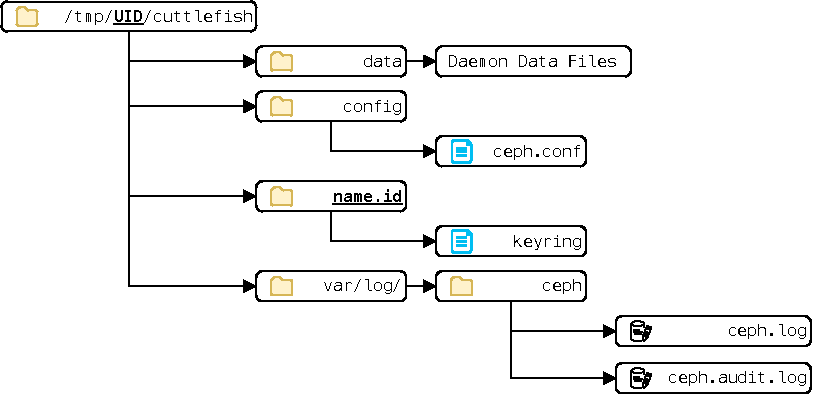
\includegraphics[width=\linewidth]{assets/cuttlefish/file_folder_layout.pdf}
        \caption[Daemon File/Folder Layout]{File and folder layout of a daemon deployed using Cuttlefish. The \texttt{ceph.conf} file is shared across all daemons, while the keyring is generated per-daemon from the full keyring stored in the manifest. The data folder contains data generated and/or required by Ceph for that specific daemon. Monitors write to the \texttt{ceph.log} and \texttt{ceph.audit.log} files.}
        \label{fig:daemon-file-folder-layout}
    \end{figure}
    
    \item The configuration is extracted from the manifest and written to \texttt{config/ceph.conf}, used by all nodes.
    \item The keyring is extracted from the manifest, and only the key for the daemon is placed in the daemon's folder, e.g., \texttt{osd.0/keyring}. For monitors, the entire keyring with the pre-generated keys for all daemons is provided, even if only a subset of daemons defined in the keyring are deployed.
    \item Monitors and \acp{OSD} are initialized if their data directories are empty with the \texttt{-{}-mkfs} commands for each daemon.
    \item Daemons are started in the order of: monitors, managers, \acp{OSD}, \acp{MDS}, followed by other daemons (if any) as Apptainer instances with the appropriate folders mounted.
\end{itemize}

After these steps are completed, each node will run its assigned daemons within independent Apptainer instances. An example is shown in \Cref{lst:apptainer_instance_list}, shortened for brevity.

\lstinputlisting[
    caption={Apptainer Instance Listing for Running Cluster},
    label={lst:apptainer_instance_list},
    frame=single,
    breaklines=true
]{assets/cuttlefish/apptainer_instance_list.txt}

To confirm that all instances are running, the layout of running instances can be requested from the deployment script, as shown in \Cref{lst:daemon_get_state}. This must be performed from a machine with \ac{SSH} access to and login permissions for the member nodes.

\lstinputlisting[
    caption={Listing of Running Daemons},
    label={lst:daemon_get_state},
    frame=single,
    breaklines=true
]{assets/cuttlefish/daemon_get_state.txt}

\subsubsection{Teardown}

Teardown follows the same process as deployment, using the deployment controller
script with the command shown in~\cref{lst:daemon-teardown}.

\lstinputlisting[
    caption={[Cluster Teardown]{Command used to tear down a Ceph cluster. This command stops all Ceph daemon containers as defined in the manifest, followed by the deletion of the folder structure generated in~\cref{fig:daemon-file-folder-layout}.}},
    label={lst:daemon-teardown},
    frame=single,
    breaklines=true
]{assets/cuttlefish/teardown.txt}

Note that this command does not cancel the Slurm job. The cluster can be re-deployed immediately: either with the same manifest, or with a manifest generated using different parameters, e.g., more \acp{OSD} or a different distribution of daemons on the cluster nodes within the allocated Slurm job.


\subsection{Production Deployment}
\label{sec:production-deployment}

In addition to Ceph performance testing, we intend to evaluate Ceph from a systems administration perspective. In order to do so, it is necessary to test Ceph's production-ready components, such as cephadm and BlueStore, to evaluate the following functionality:

\begin{itemize}
    \item Ease of deployment from scratch
    \item Processes involved in adding and removing storage from the cluster
    \item Enablement of various Ceph services
    \item Performance characteristics
\end{itemize}

Note that, unlike~\cref{sec:custom-deployment}, the performance characteristics being referred to in this section are not intended to test Ceph's performance limits, as the hardware available for this rootful production deployment is significantly more performance-limited than that available for the custom deployment. Instead, the intent is to evaluate how Ceph interacts with hardware under well-known, controlled lab conditions. To that end, we will control factors such as \ac{OSD} layout and disk \ac{I/O} performance in order to compare Ceph's theoretical behaviour with observed behaviour.

\subsubsection{Deployment Hardware}

The deployment consists of a test cluster with 8 nodes, which are configured as
virtual machines on a single host, shown in~\cref{tab:dev-cluster}.

\begin{table}[h!]
    \centering
    \begin{tabular}{|ll|}
        % \multicolumn{2}{Host Hardware} \\
        \hline
        \multicolumn{2}{|l|}{\textbf{Host Details}} \\
        \hline
        Host \ac{OS}        & Cent\acs{OS} Stream 9 \\
        \ac{CPU}            & Intel Xeon E5-1650 v3 (6 cores, 12 threads) \\
        \ac{RAM}            & 256 GiB \\
        Disk                & 2x 480 GB \acs{RAID} 0 \ac{SSD} \\
        Ceph vDisk Storage  & 128 GiB \texttt{tmpfs} \\
        \hline
        % \multicolumn{2}{Guest Hardware}
        \multicolumn{2}{|l|}{\textbf{Guest Details}} \\
        \hline
        Hypervisor          & Linux KVM via libvirt \\
        Hostnames           & cvm[1-8] \\
        \acs{IP} Addresses  & 10.1.1.[1-8] \\
        v\acs{CPU}s         & 4 (2 cores, 4 threads) \\
        \acs{RAM}           & 16 GiB \\
        Boot Disk           & 100 GiB Virt\acs{IO} Block \\
        Ceph vDisk          & 16 GiB Virt\acs{IO} Block on \acs{RAM}-backed tmpfs \\
        Guest \acs{OS}      & Cent\acs{OS} Stream 9 \\
        Networking          & Virt\acs{IO} \\
        \hline
    \end{tabular}
    \caption[Development Cluster Hardware]{The development cluster used for system evaluation and lab-controlled performance testing.}
    \label{tab:dev-cluster}
\end{table}

\subsubsection{Performance Throttling}

We will primarily be evaluating how well Ceph performs with a known upper limit to disk performance. Libvirt supports setting \ac{I/O} limits per disk based on user-specified \ac{IOPS} or bandwidth targets, as well as other, more granular options as shown in~\cref{lst:blkdeviotune}.

\lstinputlisting[
    caption={
        [VirtIO Block Device Throttling]
        Available options for the \texttt{virsh blkdeviotune} command for throttling disk performance.
    },
    label={lst:blkdeviotune},
    frame=single,
    breaklines=true
]{assets/virt/blkdeviotune.txt}

The throttling can be validated in the virtual machines by running a tool such
as hdparm or \ac{FIO}, as shown in~\cref{lst:hdparm-fio-throttling}.

\lstinputlisting[
    caption={
        [Throttling Validation with fio/hdparm]
        Validation of a read limit of 50 MiB/s ($\approx$52.43 MB/s), performed with fio and hdparm. Only the summary is shown in the fio output for clarity.
    },
    label={lst:hdparm-fio-throttling},
    frame=single,
    breaklines=true
]{assets/virt/fio-check-speed.txt}

\subsection{Network Optimization}

The performance of any networked file system is fundamentally limited by the underlying network on which the file system communicates. The network's characteristics, such as latency and throughput, impose a theoretical upper bound on the file system's capabilities. To distinguish between the limitations imposed by Ceph's architecture and that of the network hardware, this section establishes our methodology for tuning network performance and establishing a throughput baseline.

Ceph deployments do not utilize \ac{RDMA} by default for communication, in contrast to \acs{HPC}-native file systems such as Lustre and BeeGFS. While \ac{RDMA} is a common feature in \ac{HPC} networking hardware, Ceph relies on the standard \ac{TCP/IP} stack for its communication. The use of \ac{TCP/IP} over \ac{RDMA} introduces several performance trade-offs~\cite{linux_kernel_networking}:

\begin{itemize}
    \item \ac{TCP/IP} processing is primarily performed in software, incurring significant performance costs at high throughputs through packet processing and context switching overhead.
    \item \ac{RDMA} performs zero-copy transfers, which allow for direct placement of data from the network adapter to application memory. However, \ac{TCP/IP} performs multiple buffer copies throughout the networking stack before reaching user space, incurring additional overhead.
    \item The aforementioned kernel overhead and memory copies lead to increased \ac{CPU} usage, reducing the compute performance available for \ac{HPC} workloads.
\end{itemize}

Consequently, Ceph incurs a \ac{CPU} utilization and network throughput disadvantage compared to \ac{HPC} file system competitors, inherent to its use of \ac{TCP/IP} for communication. Additionally, the modeling of \ac{TCP} performance can be more complex, as it depends on several additional factors beyond theoretical link speed:

\begin{itemize}
    \item Network type (Ethernet, InfiniBand, etc.)
    \item Kernel version and driver version, since newer kernels may have more optimized networking code
    \item Performance of the \ac{CPU}, including factors such as its clock speed, core count, memory layout, and internal interconnect bandwidth
    \item The offloads available and used on the network adapter
    \item Tunable parameters, such as:
    \begin{itemize}
        \item \ac{MTU}
        \item Congestion control algorithms
        \item Interrupt handling and steering
        \item Message buffer sizes
    \end{itemize}
\end{itemize}

While these factors can also affect \ac{RDMA} transports, the offloading of data transport operations to network hardware mitigates much of the performance variability which can arise from host-side bottlenecks. Therefore, in the context of this thesis, the performance baselines established are intended for comparative measurements on identical hardware, rather than an absolute metric for peak performance. The following subsections cover the optimizations applied to Omni-Path and InfiniBand, as these interconnects are used in the \ac{GWDG} \ac{HPC} cluster nodes.

\subsection{Omni-Path Optimizations}
\label{sec:opa-optimization}

The majority of the production nodes used in the \ac{HPC} cluster of the \ac{GWDG} are
equipped with Omni-Path networking, and a small number with InfiniBand
networking. However, we will focus primarily on Omni-Path, as it exhibited
architectural limitations which had a significant negative impact on the
\ac{TCP} performance available over the transport. We will focus on
the configuration and issues which were particularly impactful.

Initial testing was performed on the default Omni-Path configuration on the
\ac{GWDG} computing center. The results from these tests were poor, with 
inconsistent \ac{TCP} throughput of under 20 Gbps. The configuration and
performance results are unchanged from tests previously performed on the same
hardware~\cite{using-hpc-networks}. 

\subsubsection{Recommended Optimizations}

The Cornelis optimization guide for Omni-Path~\cite{omni-path-tuning-guide}
recommends tuning the following options in order to improve the performance of
\ac{TCP/IP} over the fabric:

\begin{itemize}
    \item Adjust the \ac{MTU} of the network interface\footnote{\cite[pp.~71--75]{omni-path-tuning-guide}}
    \item Enable \ac{GSO}\footnote{\cite[pp.~76--77]{omni-path-tuning-guide}}
    \item Enable either \ac{RPS}, or Accelerated \ac{IP} without \ac{RPS}\footnote{\cite[p.~77]{omni-path-tuning-guide}}
    \item Adjust the system \ac{TCP} parameters\footnote{\cite[p.~77]{omni-path-tuning-guide}}
    \item Enable irqbalance and adjust \ac{CPU} affinity\footnote{\cite[p.~19,~pp.~81--84]{omni-path-tuning-guide}}
    \item Enable \ac{THP}\footnote{\cite[p.~24]{omni-path-tuning-guide}}
    \item Set the \ac{IOMMU} type to pass-through mode\footnote{\cite[pp.~23--24]{omni-path-tuning-guide}}
    \item Change the \ac{CPU} performance profile to disable power saving features\footnote{\cite[pp.~19--23]{omni-path-tuning-guide}}
    \item Tune the kernel parameters \texttt{num\_sdma} and \texttt{krcvqs}\footnote{\cite[pp.~34--37,~pp.~75--76]{omni-path-tuning-guide}}
    \item Enable accelerated \ac{RDMA}\footnote{\cite[pp.~62--64]{omni-path-tuning-guide}}
    \item Tune the \texttt{ib\_ipoib} kernel module\footnote{\cite[p.~76]{omni-path-tuning-guide}}
\end{itemize}

These optimization steps were mostly applied according to the steps mentioned in
the manual. However, to preserve interoperability with the existing InfiniBand
network, it was not possible to set the \ac{MTU} larger than 4KB, and additional
issues were faced when implementing accelerated \ac{IP} support in particular.
On the Omni-Path network adapter, there are 160 available receive contexts.
These contexts are consumed by kernel, netdev, and user queues. On systems where
the number of threads nears or exceeds this limit, the number of user queues are
adjusted accordingly. However, the module does not take into account any netdev
contexts, which are required for accelerated \ac{IP} functionality. The number
of threads on the test systems (192) exceeds the context limit, which caused
accelerated \ac{IP} to fail with a message that does not directly suggest that
this system is affected, as shown in
\Cref{lst:hfi1-dmesg}.

\lstinputlisting[
    caption={hfi1 Kernel Log Output},
    label={lst:hfi1-dmesg},
    frame=single,
    breaklines=true
]{assets/network/hfi1_dmesg.txt}

After manually adjusting the value for \texttt{num\_user\_contexts} to a lower
value, the netdev contexts were allocated correctly. After applying the steps in
the guide, performance was improved. However, although the average performance
was higher, the performance results remained inconsistent. A summary of the
system configuration can be found in~\cref{tbl:opa-parameters}.

\begin{table}[h]
\centering
\begin{tabular}{ll}
\hline
\textbf{Parameter}                      & \textbf{Value} \\
\hline
\ac{MTU}                                & 4000 \\
\ac{GSO}                                & Enabled \\
Accelerated \ac{IP}                     & Enabled \\
\ac{RPS}                                & Disabled \\
\texttt{irqbalance}                     & Enabled \\
\ac{THP}                                & Always \\
\ac{CPU} Scaling Governor               & Performance \\
\hline
\textbf{Kernel Parameter}               & \textbf{Value} \\
\hline
\texttt{iommu}                          & \texttt{pt} (Passthrough) \\
\texttt{hfi1.num\_sdma}                 & 16 \\
\texttt{hfi1.num\_user\_contexts}       & 140 \\
\texttt{hfi1.krcvqs}                    & 4 \\
\texttt{ib\_ipoib.recv\_queue\_size}    & 8192 \\
\texttt{ib\_ipoib.send\_queue\_size}    & 8192 \\
\hline
\textbf{Sysctl Parameter}               & \textbf{Value} \\
\hline
\texttt{net.ipv4.tcp\_rmem}             & 16384 131072 16777216 \\
\texttt{net.ipv4.tcp\_wmem}             & 16384 16384 16777216 \\
\texttt{net.ipv4.rmem\_max}             & 16777216 \\
\texttt{net.ipv4.wmem\_max}             & 16777216 \\
\texttt{net.core.somaxconn}             & 2048 \\
\texttt{net.ipv4.tcp\_mtu\_probing}     & 1 \\
\texttt{net.core.netdev\_max\_backlog}  & 250000 \\


\hline
\end{tabular}
\caption{Configured Parameters for Omni-Path}
\label{tbl:opa-parameters}
\end{table}

\subsubsection{\acs{TCP/IP} Offload Issues} 

Similarly to InfiniBand, Omni-Path runs best on its native \ac{RDMA} capable transport, \ac{PSM}. The distinguishing factor is that, even though \ac{TCP/IP} is a \enquote{non-optimal} transport for InfiniBand, modern adapters nonetheless provide hardware offloads for it. Stateless offloads have also been the norm on Ethernet adapters to the extent that, in addition to datacenter Ethernet adapters, commodity Ethernet adapters support such offloads as well\footnote{Ethernet adapter tested: Realtek RTL8111.}.

\Cref{tbl:nic-offload} shows a summary of the supported capabilities of  selected network adapters by network type, relevant for \ac{TCP/IP}, gathered using ethtool\footnote{Omni-Path Adapter: Intel 100HFA016 / 1x100Gb, InfiniBand Adapter: ConnectX-6 MT28908 / 2x200Gb, Ethernet Adapter: ConnectX-6 Dx MT2892 / 2x25GbE ports, Commodity Ethernet Adapter: Realtek RTL8111 / 1x1GbE port}.

\begin{table}[h!]
\centering
% \resizebox{\textwidth}{!}{
\begin{tabular}{lccc}
\hline
\textbf{Offload} & 
\textbf{Omni-Path} &
\textbf{Ethernet} &
\textbf{InfiniBand}
\\
\hline
Scatter-Gather                           & \checkmark & \checkmark & \checkmark \\
Generic Segmentation (GSO)               & \checkmark & \checkmark & \checkmark \\
Generic Receive (GRO)                    & \checkmark & \checkmark & \checkmark \\
RX Checksum                              &            & \checkmark & \checkmark \\
TX Checksum                              &            & \checkmark & \checkmark \\
TCP Segmentation (TSO)                   &            & \checkmark & \checkmark \\
VLAN                                     &            & \checkmark & \checkmark \\
Receive Hashing                          &            & \checkmark & \checkmark \\
\hline
\end{tabular}
% } % resizebox
\caption{NIC Offload Capabilities}
\label{tbl:nic-offload}
\end{table}

It should be noted that \ac{GRO} and \ac{GSO} are not \enquote{offloads} in the
traditional sense. These offloads are not performed by the network adapter
hardware, but rather the kernel itself in
software~\cite{linux-doc-segmentation-offloads}. The lack of offloads results in
high \ac{CPU} overhead for packet processing, and in particular the lack of
receive hashing has a pronounced effect on the way this processing is
distributed across available cores on the system.

\subsubsection{Interrupt Handling Issues}
\label{sec:interrupt-handling-issues}

\Cref{fig:opa-irq} demonstrates the \ac{CPU} bottleneck issue during the performance testing, where one core is pinned at 100\% \acs{CPU} usage. In this specific instance, performance was highly variable, often ranging between 15-45\ Gbps. As a result, the performance of \ac{TCP} over Omni-Path is significantly lower than the network adapter's physical throughput limit of 100\ Gbps. Note that this figure only displays the 24 cores which displayed non-zero utilization; the remaining cores of the 92-core, 192-thread system were idle.

\begin{figure}[h]
    \centering
    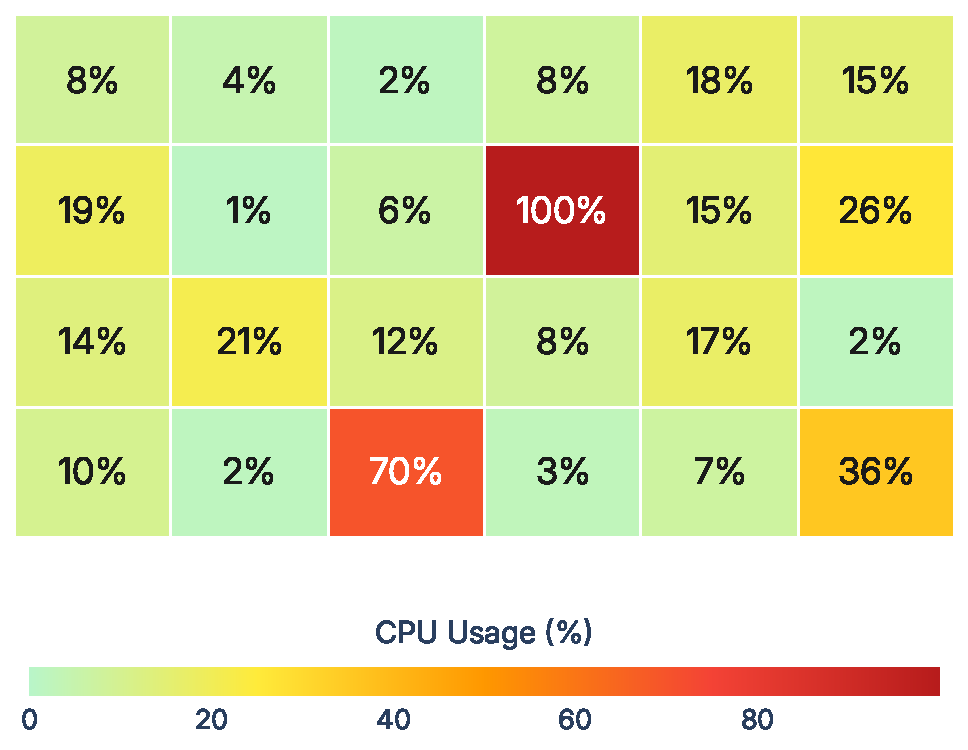
\includegraphics[width=0.5\linewidth]{assets/network/omni_path_cpu_heatmap.pdf}
    \caption[Omni-Path CPU Usage Heatmap]{Heatmap showing all cores with non-zero utilization during performance testing of Omni-Path. The heatmap demonstrates that a single core is fully loaded, while most other cores remain idle or lightly loaded.}
    \label{fig:opa-irq}
\end{figure}

The Omni-Path tuning guide also provides a method for determining the mapping of cores to interrupts~\cite{omni-path-tuning-guide}. Using this, we are able to determine which interrupt types place the most load on the \ac{CPU}. The interrupt mapping is shown in~\cref{fig:omni-path-irq-layout}.

\begin{figure}[H]
    \centering
    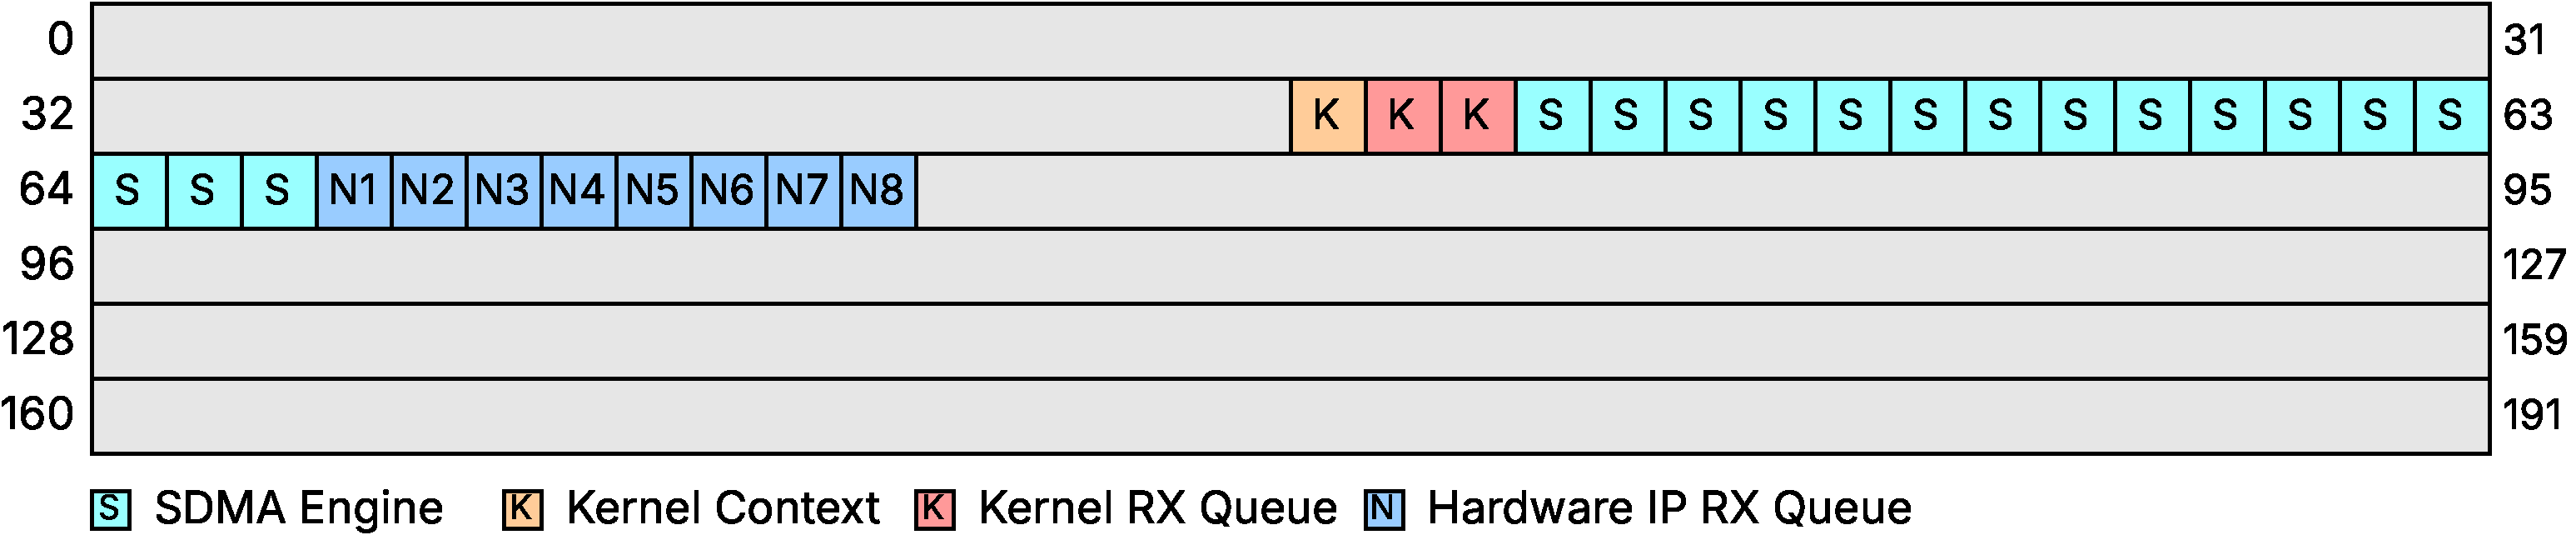
\includegraphics[width=\linewidth]{assets/network/rps/Interrupt-Layout.pdf}
    \caption{Omni-Path IRQ Layout}
    \label{fig:omni-path-irq-layout}
\end{figure}

Based on the interrupt mapping, the performance bottleneck likely stems from the \ac{CPU} usage of interrupts generated to service regular \ac{IP} traffic. This demonstrates that the processing overhead of \ac{IP} over Omni-Path is high due to the interrupt processing. More critically, despite the large number of cores---and therefore, theoretically available network processing performance---the single-core performance remains a performance bottleneck.

Beyond Ceph, these performance limitations can be of particular concern for high-bandwidth \ac{IP} traffic producers and consumers. On the \ac{GWDG} \ac{HPC} cluster, there is an additional network architecture constraint of a 4KB \ac{MTU} for interoperability with InfiniBand hardware, which further increases packet count compared to the maximum supported Omni-Path \ac{MTU} of 10KB. Furthermore, the \acp{CPU} used in the \ac{HPC} cluster are high-core-count \acp{CPU}, which generally have reduced single-core performance compared to, e.g., low-core-count consumer-grade \acp{CPU}. For instance, a consumer-grade Intel \ac{CPU} may run at 6 GHz, while a server-grade \ac{CPU} released during the same time frame may run at 4.1 GHz\footnote{Data from Intel ARK: \url{https://www.intel.com/content/www/us/en/ark.html}. Accessed 03.02 2026. Consumer \acs{CPU}: i9-14900K; Server \acs{CPU}: Xeon Gold 6538N.}.

\subsubsection{Enabling \acs{RPS} with Accelerated \acs{IP}}

The Omni-Path optimization guide recommends enabling either \ac{RPS} or
Accelerated \ac{IP} \cite[p.~77]{omni-path-tuning-guide}. However, given the
interrupt load shown in~\cref{sec:interrupt-handling-issues} as well as the
suboptimal performance, an experimental evaluation of \ac{RPS} in combination
with Accelerated \ac{IP} was performed. To that end, a specialized script was
developed to automatically assign available cores to network queues under the
following constraints:

\begin{itemize}
    \item \ac{RPS} flows can be placed on the same \ac{NUMA} node as the original interrupts to minimize latency, or spread across multiple nodes to potentially improve throughput.
    \item The number of \ac{RPS} flows, as well as the cores on which these \ac{RPS} flows are placed, are adjusted such that they do not overlap with existing interrupts.
    \item The hardware thread for each core is taken into consideration during the placement process to prevent overlaps with the same \ac{CPU} core.
\end{itemize}

\ac{RPS}
flow policies both with and without \ac{NUMA} restrictions were used. The
\ac{NUMA}-restricted placement policy has fewer cores available for \ac{RPS}
flows. However, it benefits from higher bandwidth due to its memory and network
adapter locality. The placement is shown in~\cref{fig:rps-single-numa}.

\begin{figure}[H]
    \centering
    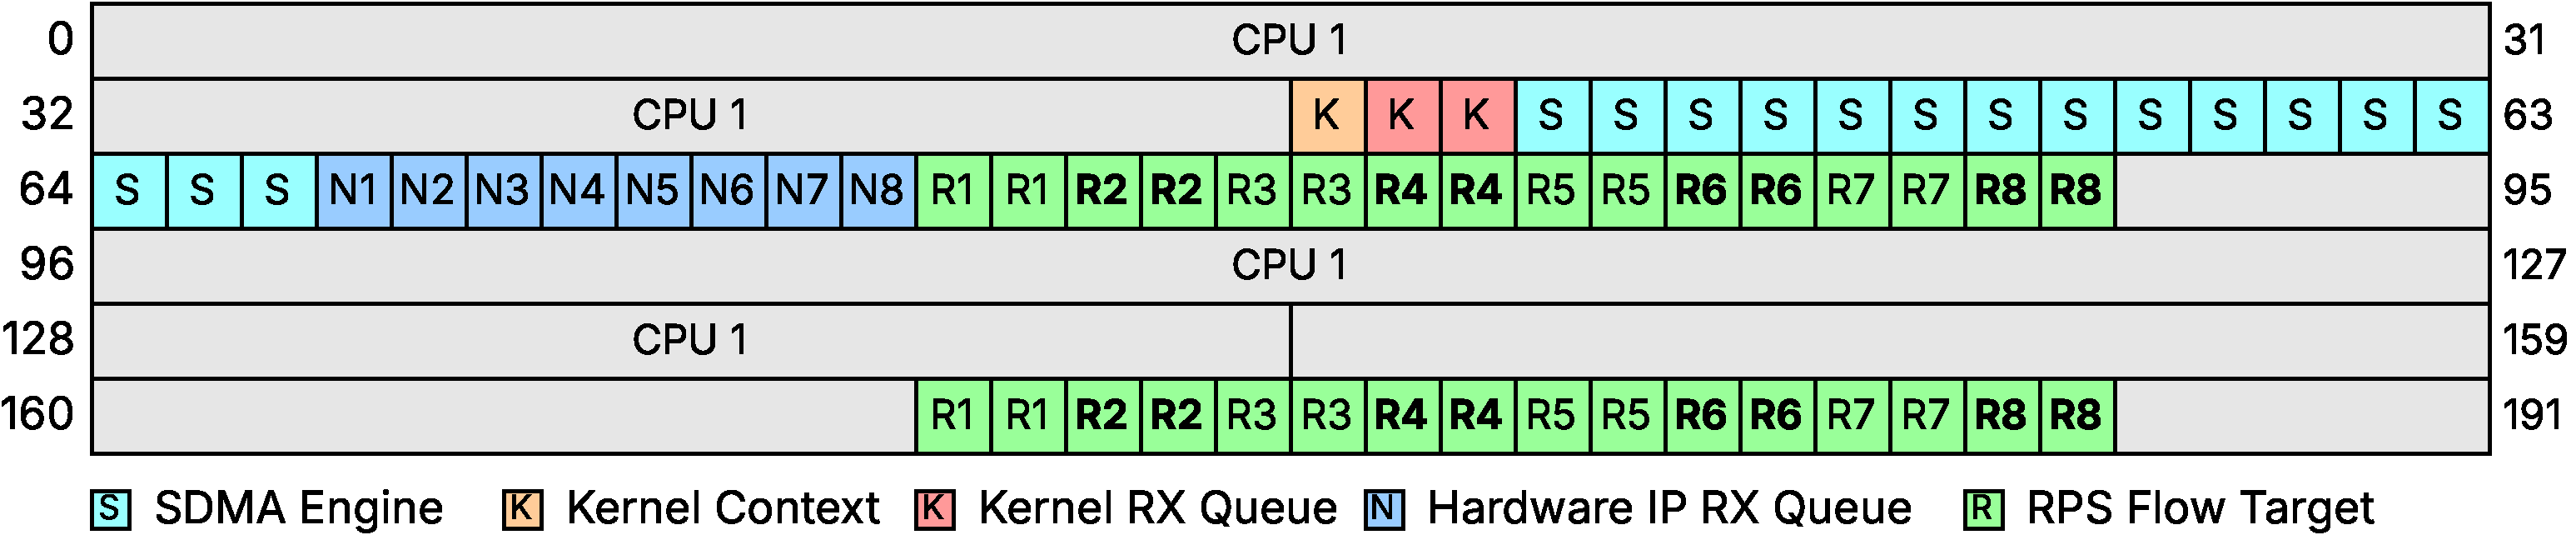
\includegraphics[width=\linewidth]{assets/network/rps/RPS-Single-NUMA.pdf}
    \caption{Single-\acs{NUMA}-Node \acs{RPS} Configuration}
    \label{fig:rps-single-numa}
\end{figure}

The unrestricted \ac{RPS} flow placement is shown in~\cref{fig:rps-multi-numa}.
It has significantly more cores per hardware interrupt to work with, but could
potentially perform worse due to the latency and bandwidth constraints
introduced by the inter-\ac{NUMA}-node link.

\begin{figure}[H]
    \centering
    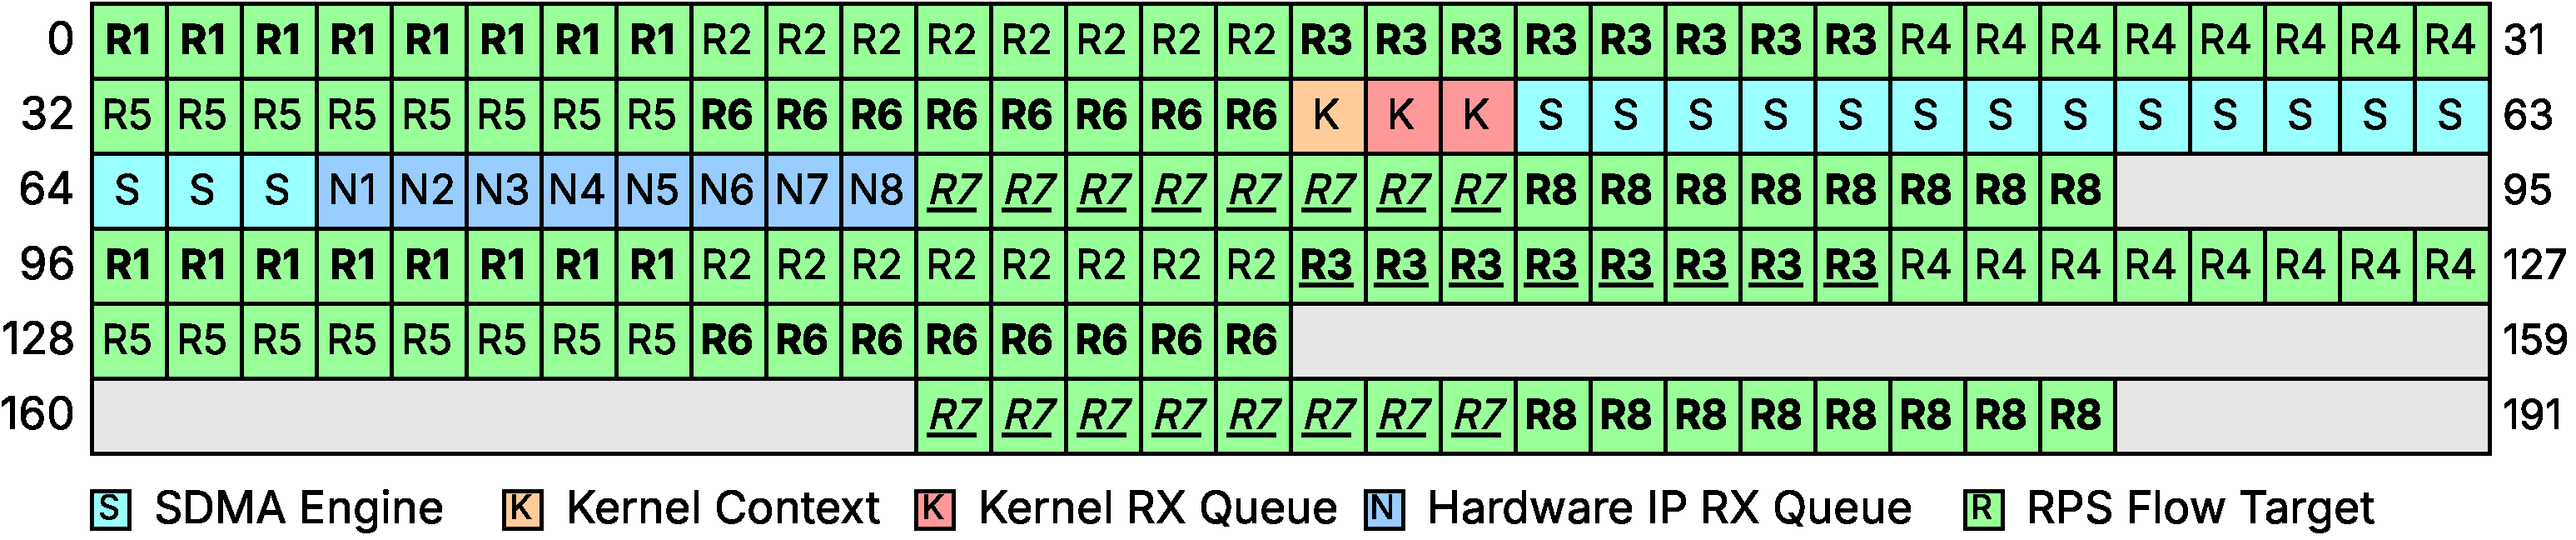
\includegraphics[width=\linewidth]{assets/network/rps/RPS-Multi-NUMA.pdf}
    \caption{Multi-\acs{NUMA}-Node \acs{RPS} Configuration}
    \label{fig:rps-multi-numa}
\end{figure}

% These optimizations were applied to the test nodes and initial testing was
% performed between two Omni-Path equipped test nodes
% (see~\cref{tbl:omnipath-system} for specifications). However, the observed
% performance results were poor.

\subsection{InfiniBand Optimizations}

InfiniBand supports Ceph's \ac{TCP/IP} traffic through its \ac{IPoIB} protocol. While all optimizations as shown in~\cref{tbl:nic-offload} for InfiniBand network adapters were enabled on the tested nodes, the \ac{MTU} was restricted to a maximum of 4000 bytes in order to preserve compatibility with existing infrastructure, such as storage servers and network switches. \Cref{tbl:infiniband-parameters} details the tuned system configuration applied to the test nodes, which were equipped with 200 Gbit/s NVIDIA ConnectX-6 adapters operating in InfiniBand mode.

\begin{table}[h]
\centering
\begin{tabular}{ll}
\hline
\textbf{Parameter}                      & \textbf{Value} \\
\hline
\ac{MTU}                                & 4000 \\
\ac{RPS}                                & Disabled \\
\texttt{irqbalance}                     & Enabled \\
\ac{THP}                                & Always \\
\ac{CPU} Scaling Governor               & Performance \\
\hline
\textbf{Kernel Parameter}               & \textbf{Value} \\
\hline
\texttt{iommu}                          & \texttt{pt} (Passthrough) \\
\texttt{ib\_ipoib.recv\_queue\_size}    & 8192 \\
\texttt{ib\_ipoib.send\_queue\_size}    & 8192 \\
\hline
\textbf{Sysctl Parameter}               & \textbf{Value} \\
\hline
\texttt{net.ipv4.tcp\_rmem}             & 16384 131072 16777216 \\
\texttt{net.ipv4.tcp\_wmem}             & 16384 16384 16777216 \\
\texttt{net.ipv4.rmem\_max}             & 16777216 \\
\texttt{net.ipv4.wmem\_max}             & 16777216 \\
\texttt{net.core.somaxconn}             & 2048 \\
\texttt{net.ipv4.tcp\_mtu\_probing}     & 1 \\
\texttt{net.core.netdev\_max\_backlog}  & 250000 \\


\hline
\end{tabular}
\caption{Configured Parameters for InfiniBand}
\label{tbl:infiniband-parameters}
\end{table}

Manual tuning of software interrupt handling, i.e., \ac{RPS}, was not considered necessary. In contrast to Omni-Path's capabilities, the InfiniBand network adapters supported hardware receive hashing/flow steering with 64 dedicated queues each for send and receive operations, compared to the 8 supported by Omni-Path.

\subsection{Benchmarking Goals}

The benchmarking methodology developed for this thesis is designed for the evaluation of the Ceph file system across diverse cluster configurations in order to assess its suitability for \ac{HPC} applications. To that end, we have deployed and evaluated two classes of Ceph clusters:

\begin{itemize}
    \item A simulated production environment (see~\cref{sec:production-deployment}), deployed with \texttt{cephadm}
    \item Custom in-memory deployments (see~\cref{sec:custom-deployment}), deployed with the Cuttlefish deployment tool developed for this thesis
\end{itemize}

In the production deployment, our benchmarking objectives are primarily qualitative and architectural evaluations. This deployment does not focus on peak performance measurements, as the constraints of the production deployment are controlled such that they are not expected to exceed Ceph's architectural capabilities. Instead, we have evaluated the orchestration process using \texttt{cephadm}, as well as analyzed potential deviations between theoretical performance models controlled by our performance throttling process and the observed behaviour of the cluster.

The in-memory deployment focuses primarily on quantitative stress testing in order to isolate Ceph's architectural performance limitations. These benchmarks are designed to evaluate Ceph's performance and scalability at various levels under high-load conditions, eliminating external compounding factors where possible. For instance, physical storage media such as hard drives and \acp{SSD} can have complex and potentially non-deterministic performance characteristics; using memory-backed \acp{OSD} eliminates disk performance as a source of potential performance bottlenecks. This methodology allows for an evaluation focused primarily on software overhead of the various layers of the Ceph file system, such as \ac{RADOS} and \ac{CephFS}, although other limiting factors such as memory and network bandwidth remain. 

\ac{IOR} and mdtest benchmark configurations were repeated 3 and 5 times respectively to account for random network jitter and other sources of variance. The higher repetition count for mdtest was chosen due to the higher observed variance in metadata operations compared to \ac{IOR}'s throughput measurements. Unless stated otherwise, the reported results are the mean across repetitions.

\subsubsection{Performance Testing}

Performance was evaluated through performance metrics obtained via two of its primary interfaces: the \ac{RADOS} object storage layer and \ac{CephFS}.

\ac{RADOS} performance benchmarks were used to establish a fundamental performance baseline, as it serves as the underlying storage method for all higher-level Ceph services, such as \ac{CephFS}, \ac{RBD}, and \ac{RGW}. As such, these measurements represent a theoretical \enquote{upper bound} of the cluster's throughput and \ac{I/O} capabilities at the lowest abstraction level.

The evaluation additionally includes \ac{CephFS} to assess performance in real-world deployments, such as the hosting of users' home directories or a high-performance scratch file system. In these scenarios, the overhead introduced by the implementation of a \ac{POSIX} compliant file system and its associated functionality is of particular concern. We have placed particular emphasis on metadata performance, as the \ac{MDS} daemons can represent a potential bottleneck, and common workloads such as the creation of Python virtual environments or compilation of software packages produce uniquely high-frequency bursts of small file \ac{I/O}.

A comparative analysis of \ac{RADOS} and \ac{CephFS} results with the same cluster configuration allows for the quantification of the overhead introduced specifically by the \ac{CephFS} file system abstraction layer.

\subsection{Benchmark Implementation}

\subsubsection{Modifications to \acs{IOR} and mdtest}
\label{sec:modifications-to-ior-mdtest}

During initial testing, bugs and limitations in \ac{CephFS} functionality within \ac{IOR} and mdtest were discovered and patched. The following components within the \ac{CephFS} backend were modified.

\begin{itemize}
    \item Addition of \texttt{mknod} and \texttt{rename} functionality, enabling the mdtest mknod folder creation and directory renaming tests
    \item Fix for the \texttt{CEPHFS\_StatFS} function to return correct index node utilization
\end{itemize}

These fixes enable full mdtest functionality on the \ac{CephFS} backend. Note
that the \ac{RADOS} backend, being an object store, does not provide a file
system structure to be tested. Therefore, \ac{RADOS} can only be tested with
\ac{IOR}.

In addition, the outputs provided by \ac{IOR} and mdtest are insufficient for
debugging, as they report only that operations have failed without exposing
additional details, such as error codes. This lack of information made issues
such as incorrect permissions or missing folders difficult to identify. The
programs were modified to emit detailed information on failure to address this
limitation. However, it does not affect the system's functionality and exists
purely as a debugging aid.

\subsubsection{Benchmarking Container Creation}

The Ceph image does not contain \ac{IOR} or mdtest on its own, and not all of
its dependencies were straightforward to install on Rocky Linux 8. This was
primarily due to the older software versions available in the package
repositories. Therefore, these were compiled from source on top of the existing
upstream Ceph container with a Dockerfile (see~\cref{appendix:ior-mdtest-dockerfile}).

The build script performs the following:

\begin{itemize}
    \item Installs the development headers and links \ac{IOR}/mdtest to the Ceph 
libraries, ensuring a version match with the containers on the server side.
    \item Installs Open \ac{MPI} to allow for communication between \ac{IOR} tasks.
    \item Enables the optional support for \acs{CephFS} and \acs{RADOS} within \ac{IOR}.
    \item Patches \ac{IOR}/mdtest to add the functionality specified in~\cref{sec:modifications-to-ior-mdtest}
\end{itemize}

Since the Docker build process outputs a Docker image, conversion into
Apptainer's native \ac{SIF} format is required. Apptainer provides functionality
to perform this conversion natively, however, there were some permission issues
experienced when building on top of the existing Ceph image. In order to fix
this, a simple shim script was created to run an Apptainer \texttt{-{}-fix-perms}
pass on the container image, which fixed issues experienced with running dnf in
the containers during debugging. The script is shown in~\cref{lst:sif-shim-fix-perms}.

\lstinputlisting[
    caption={\acs{SIF} Conversion Shim},
    label={lst:sif-shim-fix-perms},
    frame=single,
    breaklines=true
]{assets/cuttlefish/build_ior.sh}

The output container, \texttt{cf-bench-ior.sif}, is used specifically for
benchmarking. The unmodified Ceph container image is used for the daemons.

\subsubsection{Performance Scaling}

In order to evaluate and narrow down possible sources of performance bottlenecks, we will run performance tests using different combinations of clients and nodes. For instance, if a single node with 64 tasks performs worse than two nodes with 32 tasks each, it is possible that this is not a server-side bottleneck, but rather a client-side one, e.g., a compute or network bandwidth limitation.

To that end, a custom benchmarking script was developed which automates the running of various \ac{IOR} and mdtest configurations. The system shares some core components with the deployment system, such as the the Slurm interface, in order to determine the available nodes. The benchmarks are performed on the cluster based on the user's request and node allocation, and are saved to a database for further processing. The workflow is shown in~\cref{fig:cuttlefish-benchmark-flowchart}.

\begin{figure}[htbp]
    \centering
    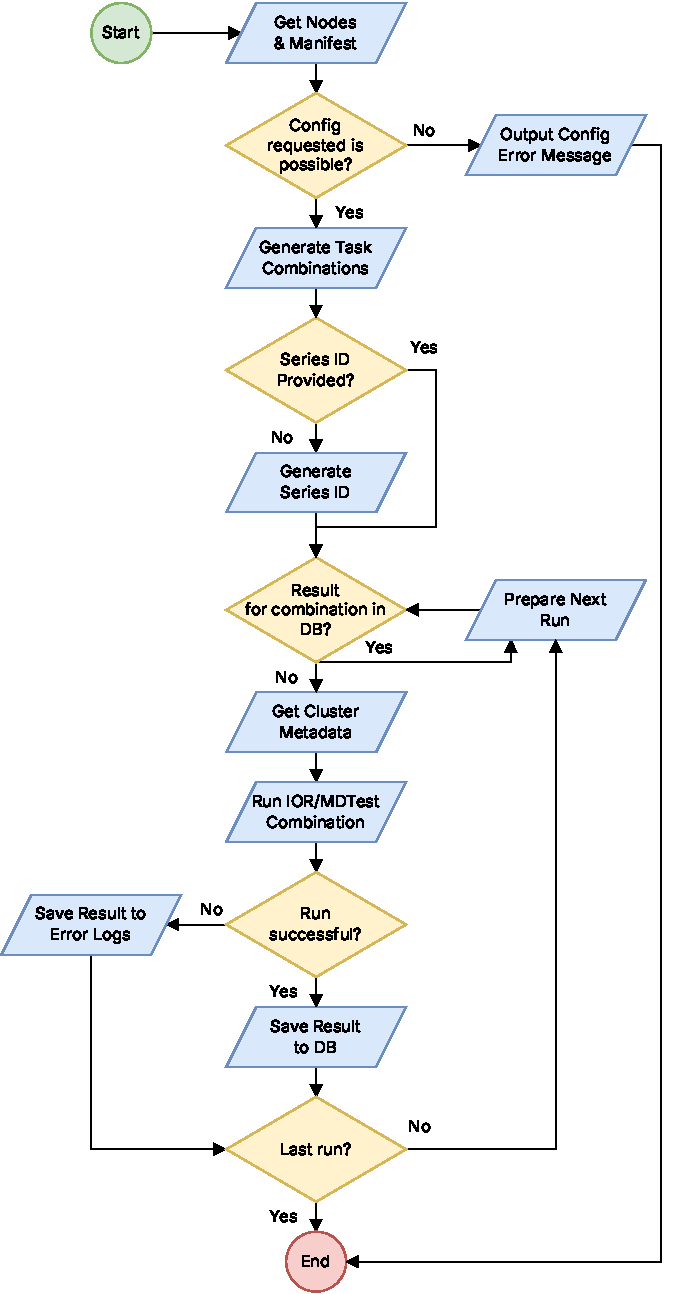
\includegraphics[width=0.7\linewidth]{assets/cuttlefish/benchmark_flowchart.pdf}
    \caption{Benchmarking Process Flowchart}
    \label{fig:cuttlefish-benchmark-flowchart}
\end{figure}

\subsubsection{Layout}

Two node types were tested: one with InfiniBand networking and one with
Omni-Path networking. All node types were running Rocky Linux 8.10 with the
kernel version 4.18.0-553.89.1.el8\_10.x86\_64.

The 16 InfiniBand test nodes were equipped with the hardware shown in
\cref{tbl:infiniband-system}.

\begin{table}[H]
\centering
\begin{tabular}{|ll|}
\hline
\textbf{Component} & \textbf{Specification} \\
\hline
CPU        & 2$\times$ AMD EPYC 7513 (32C/64T per CPU) \\
RAM        & 512 GB \\
Networking & 200 Gbps InfiniBand (NVIDIA ConnectX-6) \\
\hline
\end{tabular}
\caption{InfiniBand Test System Hardware}
\label{tbl:infiniband-system}
\end{table}

The Omni-Path nodes were equipped as shown in \cref{tbl:omnipath-system}.

\begin{table}[H]
\centering
\begin{tabular}{|ll|}
\hline
\textbf{Component} & \textbf{Specification} \\
\hline
CPU        & 2$\times$ Intel Xeon Platinum 8468 (48C/96T per CPU) \\
RAM        & 256 GB \\
Networking & 100 Gbps Omni-Path (Intel HFI100) \\
\hline
\end{tabular}
\caption{Omni-Path Test System Hardware}
\label{tbl:omnipath-system}
\end{table}

For all of the test systems, individual \acp{OSD} used the Memstore backend with
dynamic sizing, as described in~\cref{sec:ceph-autoconfig}. Due to the limited
number of available nodes, monitors are co-located with other daemon types on
the same node (e.g., \ac{MDS} daemons and \acp{OSD}).

\subsection{Data Collection}
\label{sec:data-collection}

By default, \ac{IOR} and mdtest emit human-readable data. They can also be
configured to output machine-readable data; \ac{IOR} can output \ac{JSON}
formatted data, while mdtest can output \ac{CSV} formatted data. However, some
challenges were faced when programmatically parsing the data:

\begin{itemize}
    \item Both \ac{IOR} and mdtest do not provide a formally specified data schema for their outputs, which complicates the inspection of output data.
    \item Units for bandwidth metrics in \ac{IOR} are expressed interchangeably in kilobytes and megabytes.
    \item The use of case is inconsistent throughout the output. For example, individual tests have the key \texttt{TestID}, while the test parameters have the key \texttt{testID}.
    \item Summary statistics are not directly associated with performed tests, complicating the attribution of summaries to test results for analysis.
\end{itemize}

In order to allow for easier result aggregation as well as more efficient storage of test results, data pass through a three-step process consisting of parsing, normalization, and database storage.

\subsubsection{\acs{IOR} Result Parsing}

Pydantic is used to parse \ac{IOR} results from the result \ac{JSON} data directly through conversion of field names and normalization of units. A snippet is shown in~\cref{lst:ior-result-pydantic} for a single \ac{IOR} result. Additional functions and Pydantic models are used for unit conversion and to cover the rest of the \ac{IOR} output, although they are not shown here.

\lstinputlisting[
    caption={[\acs{IOR} Result Pydantic Model]Pydantic model for the results gathered from a single \acs{IOR} repetition. Units are normalized to bytes per second, types are strongly defined, and validation of these types are performed by Pydantic. Keys use consistent snake-case throughout all models, regardless of the input case of the \acs{IOR}/mdtest data.},
    label={lst:ior-result-pydantic},
    frame=single,
    breaklines=true,
    language=python
]{assets/ior/ior_result.py}


\subsubsection{MDTest Result Parsing}

The \ac{CSV}-formatted results from mdtest cannot be parsed directly by Pydantic. Therefore, the fields are first read by the Python \texttt{csv} module, and the corresponding Pydantic models are generated using a conversion function. As opposed to \ac{IOR}, mdtest does not provide details such as the number of nodes or tasks, and therefore these must be provided separately in order for these metrics to be tracked. As the benchmarking script controls the instantiation of the mdtest runs and has the required information, this is passed through to the mdtest result parser, part of which is shown in~\cref{lst:mdtest-parser}.

\lstinputlisting[
    caption={[mdtest Result Parsing Logic]Snippet of code used to convert raw \acs{CSV} data output by mdtest into Pydantic mdtest models.},
    label={lst:mdtest-parser},
    frame=single,
    breaklines=true,
    language=python
]{assets/ior/mdtest_parser.py}

\subsubsection{Data Storage}

Once raw data have been converted into the exchange format, i.e., the Pydantic
models, they are normalized before being saved to a SQLite database. This
provides more flexibility when aggregating results due to the fact that all data
are saved in a single location and do not have to, for example, be manually read
from multiple output files. This is also more efficient for large numbers of
results, as the processing of text data (i.e., \ac{JSON}/\ac{CSV} outputs) must
only be performed once during the conversion step before being stored in an
efficient database-native format.

\begin{figure}[H]
    \centering
    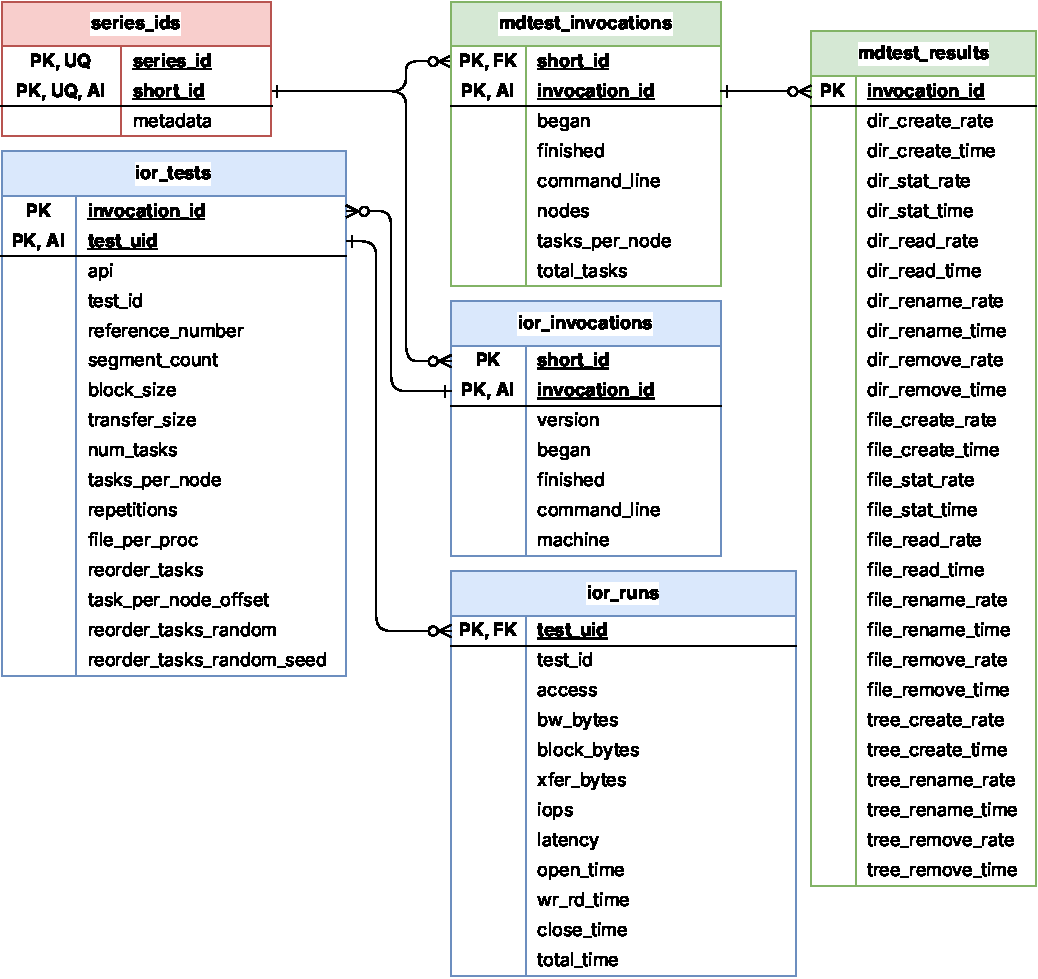
\includegraphics[width=\linewidth]{assets/cuttlefish/result-db-erd.pdf}
    \caption[Result Database ER Diagram]{\ac{ER} diagram of the result database, parsed from \acs{JSON} and \acs{CSV} data produced by \ac{IOR} and mdtest.}
    \label{fig:result-db-erd}
\end{figure}

\pagebreak

% In order to evaluate Ceph's performance characteristics, a benchmarking script
% runs multiple iterations of the \ac{IOR} benchmark with varied benchmark settings,
% numbers of client nodes and processes per node. To mimic a real-world
% deployment, the Ceph daemons and client nodes will be placed on separate
% machines. 



\section{Results}
\label{sec:results}

In this section, we will initially gather network and memory bandwidth results in order to find potential bottlenecks, followed by performance and usability evaluations of the Ceph file system.

\subsection{Network Bandwidth}
\label{sec:results-network-bandwidth}

After applying network optimizations, performance results were gathered using iperf2. Version 2 was selected specifically over iperf3 due to its mature support for multi-threading, partially mitigating \ac{CPU} bottlenecks which may be present during benchmarking. The \texttt{-P} flag was used for multithreading, and window size was set to the maximum value available on the system (\texttt{-w 32M} for 32 MB).

\subsubsection{Omni-Path}
\label{sec:results-network-bandwidth-opa}

Performance evaluation of the Omni-Path fabric reveals significant limitations in the fabric's \ac{TCP} traffic carrying capabilities. Despite the theoretical line rate being 100 Gbit/s, achievable throughput was significantly and consistently constrained by \ac{CPU} processing overheads inherent to the Omni-Path network adapters in use. Despite enabling the optimizations detailed in~\cref{sec:opa-optimization}, throughput on the \ac{GWDG} compute nodes falls far short of the theoretical limit. The performance results before and after applying various optimizations are shown in~\cref{fig:opa-tcp-throughput}.

\begin{figure}[h]
    \centering
    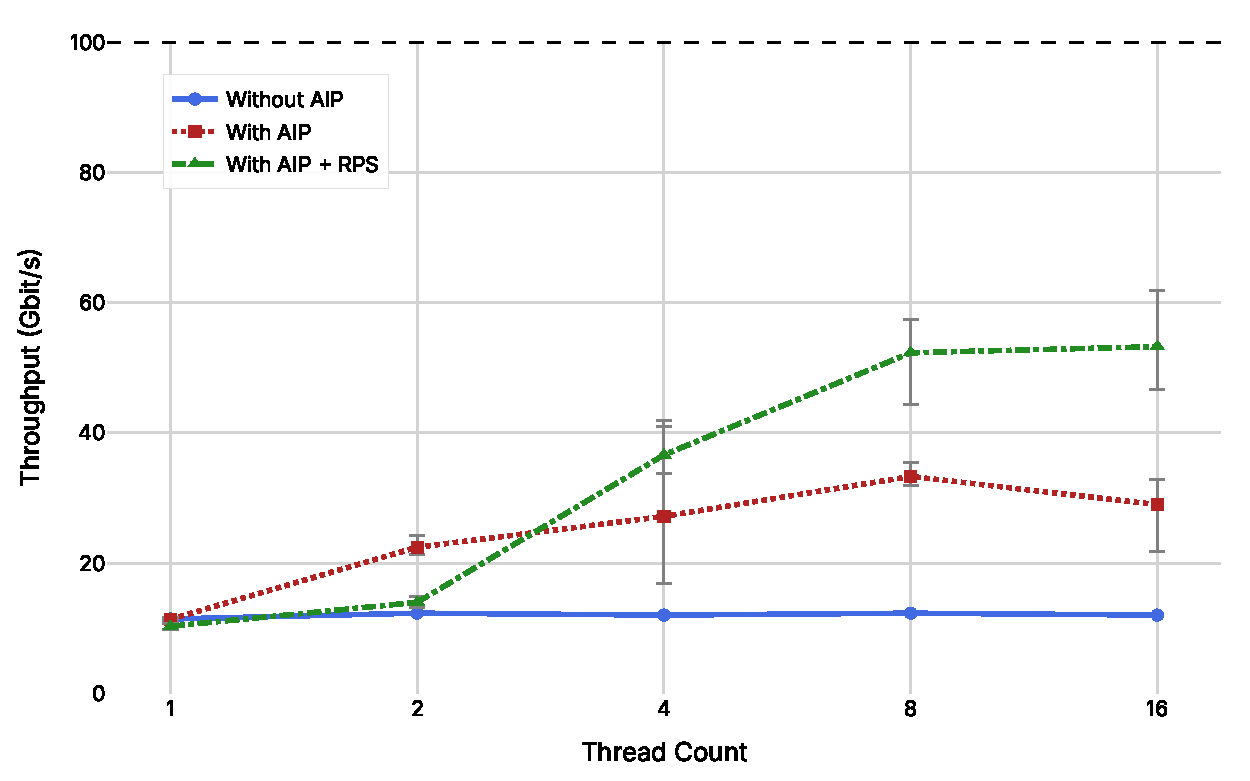
\includegraphics[width=1.0\linewidth]{assets/network/iperf/iperf_omnipath.pdf}
    \caption[Omni-Path TCP Throughput]{\acs{TCP} throughput over Omni-Path, measured using iperf2 with different parallelism settings. Despite the Accelerated \acs{IP} + \acs{RPS} method improving performance at high parallelism, the network link is underutilized.}
    \label{fig:opa-tcp-throughput}
\end{figure}

The lower performance at low thread counts with \ac{RPS} is consistent across runs. This is possibly due to the overhead of \ac{RPS} itself: the loss of cache locality and overhead of inter-processor interrupts caused by moving work to different cores may only be outweighed if the \ac{CPU} overhead of packet processing exceeds the capabilities of a single core.

As we suspect that Omni-Path performance depends highly on the performance of a single core, we performed additional testing of Omni-Path performance on consumer-grade hardware consisting of two systems, each with the hardware configuration shown in~\cref{tbl:validation-system}. These systems have the advantage over the server-grade system in that although it has less processing power overall, the per-core performance is higher; we should be able to determine if per-core performance is a bottleneck by running the benchmarks on this hardware.

\begin{table}[h]
\centering
\begin{tabular}{|ll|}
\hline
\textbf{Component} & \textbf{Specification} \\
\hline
CPU        & AMD Ryzen 9 5950X (16C/32T) \\
RAM        & 64 GB \\
Networking & 100 Gbit/s Omni-Path \\
\hline
% \multicolumn{2}{|l|}{\textbf{Memory Bandwidth Results}} \\
% \hline
% Theoretical    & 51.2 GB/s \\
% Measured       & 37.3 GB/s \\
% \hline
\end{tabular}
\caption{Validation System Hardware}
\label{tbl:validation-system}
\end{table}

Due to the limited number of cores, the number of \ac{SDMA} engines was reduced to 4, which necessitated reducing the parameter \texttt{num\_vls} to 4 as well. Accelerated \ac{IP} was enabled, and the number of user contexts was adjusted such that 6 \ac{IP} contexts were created, leaving 3 physical cores available for other tasks. The kernel parameters required to achieve this configuration are shown in~\cref{tbl:validation-system-kernel-opts}.

\begin{table}[h]
    \centering
    \begin{tabular}{|ll|}
        \hline
        \textbf{Parameter} & \textbf{Value} \\
        \hline
        \texttt{hfi1.num\_vls} & 4 \\
        \texttt{hfi1.num\_sdma} & 4 \\
        \texttt{hfi1.krcvqs} & 2 \\
        \texttt{hfi1.num\_user\_contexts} & 151 \\
        \texttt{hfi1.cap\_mask} & \texttt{0x4c09a09cbba} \\
        \hline
    \end{tabular}
    \caption[Kernel Parameters for Validation System]{Kernel parameters used for the validation system.}
    \label{tbl:validation-system-kernel-opts}
\end{table}

The interrupt layout of the validation system is shown in~\cref{fig:validation-system-irq}.

\begin{figure}[h]
    \centering
    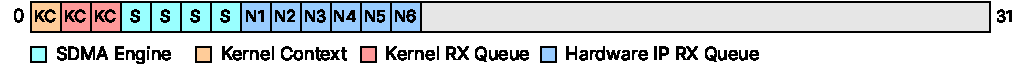
\includegraphics[width=\linewidth]{assets/network/rps/Interrupt-Layout-Ryzen.pdf}
    \caption[Validation System Interrupt Layout]{Interrupt layout of the validation system.}
    \label{fig:validation-system-irq}
\end{figure}

\Cref{fig:ryzen-opa-tcp-throughput} demonstrates the iperf throughput of the validation system with the adjusted kernel parameters and without \ac{RPS}, compared to the \ac{HPC} nodes with and without \ac{RPS}. In both cases, the validation system delivers much greater throughput than that of the \ac{HPC} nodes. However, the variance is still high: the 4-thread runs delivered between 65--93 Gbps of throughput.

\begin{figure}[H]
    \centering
    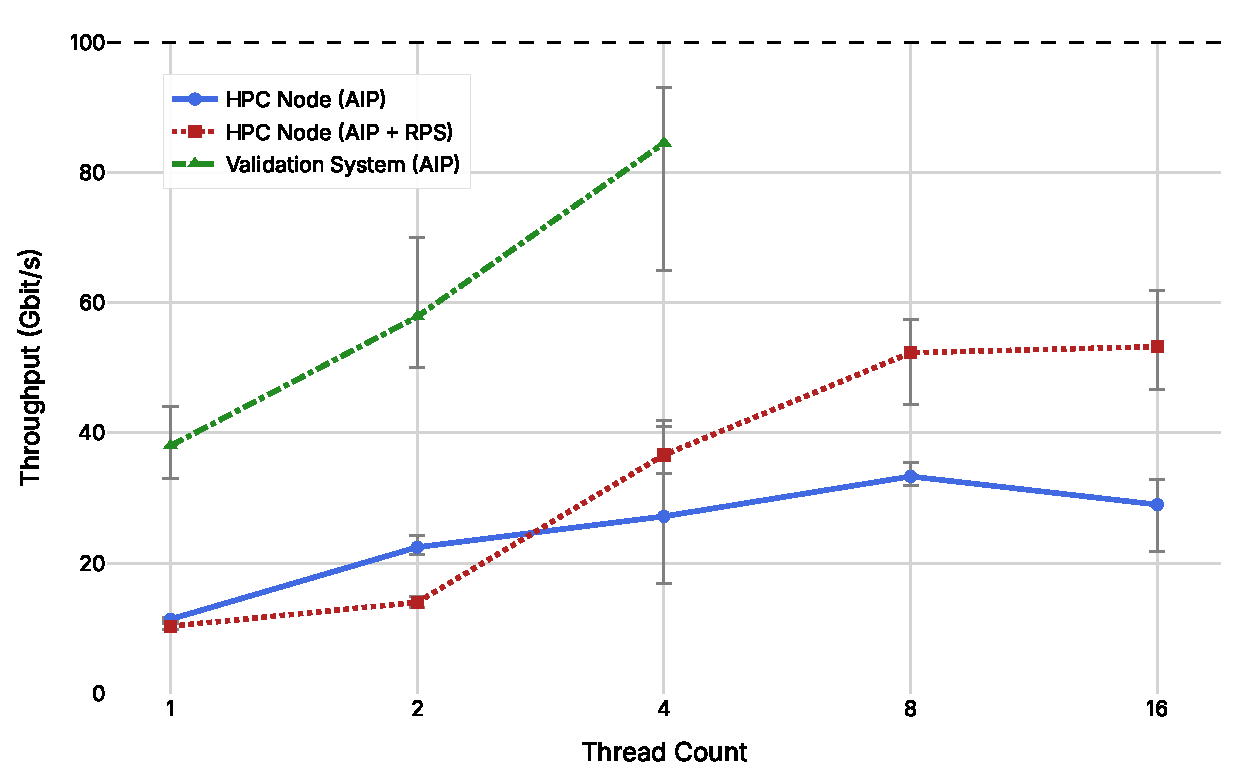
\includegraphics[width=\linewidth]{assets/network/iperf/iperf_comparison_rps_ryzen.pdf}
    \caption[Validation System TCP Performance]{\acs{TCP} throughput of the validation system. The validation systems' \ac{TCP} throughput is significantly higher than that of the \acs{HPC} nodes.}
    \label{fig:ryzen-opa-tcp-throughput}
\end{figure}

\subsubsection{InfiniBand}
\label{sec:results-network-bandwidth-ib}

\begin{figure}[H]
    \centering
    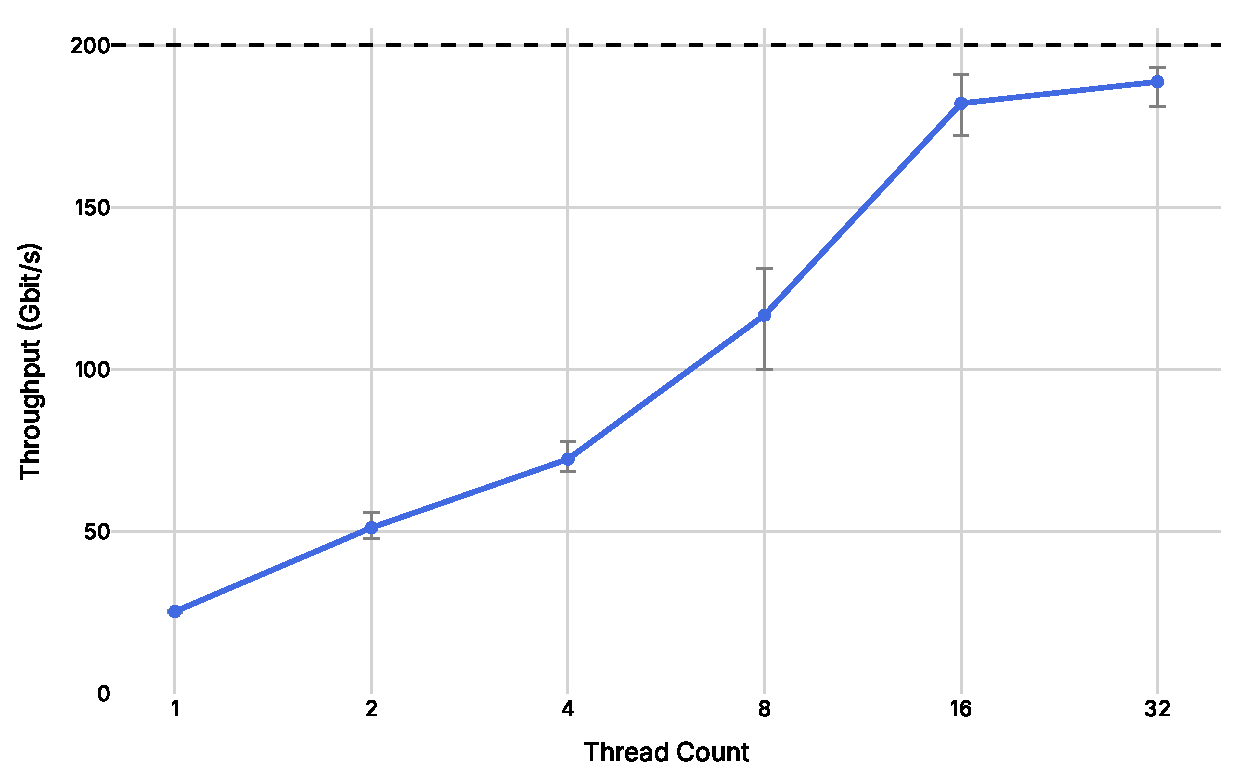
\includegraphics[width=1.0\linewidth]{assets/network/iperf/iperf_infiniband.pdf}
    \caption[InfiniBand TCP Throughput]{TCP throughput over InfiniBand, measured using iperf2 with different parallelism settings. The higher parallelism settings are capable of saturating the network link.}
    \label{fig:ib-tcp-throughput}
\end{figure}

The collected throughput results for InfiniBand are shown in~\cref{fig:ib-tcp-throughput}. A single thread achieved approximately 25 Gbit/s, whereas thread counts at or above 16 approached the theoretical network bandwidth limit of the network adapter. The peak observed throughput was 193 Gbit/s with 32 threads, representing 96.5\% of the 200 Gbit/s link speed.

During performance tests with lower thread counts, we observed iperf threads with 100\% \ac{CPU} utilization. This \ac{CPU} saturation suggests a bottleneck due to single-core processing performance, rather than a limitation of network capacity. As a result, we conclude that \ac{TCP} traffic is capable of saturating the physical network link given sufficient parallelism.

\subsection{Network Latency}

\begin{sloppypar}
For our standard network stack latency results, we used the Libfabric fi\_pingpong tool with the following options: \texttt{fi\_pingpong -e msg -I 1000} with \texttt{-p verbs} for \ac{RDMA} and \texttt{-p tcp} for \ac{TCP}, and either \texttt{-S} for message sizes of 64, 4096 (4\,KiB), or 134217728 (128\,MiB). The results are shown in~\cref{tbl:pingpong-latency} for the InfiniBand test system and~\cref{tbl:pingpong-latency-opa} for the Omni-Path test system. Note that 128\,MiB is provided as a network bandwidth test, rather than a latency test, in order to confirm \ac{RDMA} networking bandwidth.
\end{sloppypar}

\begin{table}[H]
\centering
\begin{tabular}{|lrrrr|}
\hline
\textbf{Transport} & \textbf{Size} & \textbf{Latency (\textmu{}s)} & \textbf{Bandwidth (MB/s)} & \textbf{Messages/sec} \\
\hline
\multirow{3}{*}{verbs} & 64   & 3.44  & 18.58 & 290,698.00 \\
                        & 4\,KiB   & 4.90  & 836.69 & 204,082.00 \\
                        & 128\,MiB & 6,863.50 & 19,555.30 & 145.00 \\
\multirow{3}{*}{tcp}   & 64   & 23.01  & 2.78 & 43,459.37 \\
                        & 4\,KiB   & 33.64  & 121.77 & 29,726.51 \\
                        & 128\,MiB & 60,724.00 & 2,210.30 & 16.47 \\
\hline
\end{tabular}
\caption[InfiniBand Latency Results]{Network latency results for the InfiniBand test system.}
\label{tbl:pingpong-latency}
\end{table}

\begin{table}[H]
\centering
\begin{tabular}{|lrrrr|}
\hline
\textbf{Transport} & \textbf{Size} & \textbf{Latency (\textmu{}s)} & \textbf{Bandwidth (MB/s)} & \textbf{Messages/sec} \\
\hline
\multirow{3}{*}{verbs} & 64   & 7.61  & 8.41 & 131,406.04 \\
                        & 4\,KiB   & 9.95  & 411.45 & 100,502.51 \\
                        & 128\,MiB & 27,558.80 & 4,644.75 & 36.29 \\
\multirow{3}{*}{tcp}   & 64   & 18.53  & 3.45 & 53,966.54 \\
                        & 4\,KiB   & 29.57  & 138.51 & 33,818.06 \\
                        & 128\,MiB & 130,347.60 & 1,029.69 & 7.68 \\
\hline
\end{tabular}
\caption[Omni-Path Latency Results]{Network latency results for the Omni-Path test system.}
\label{tbl:pingpong-latency-opa}
\end{table}

Overall, the InfiniBand system delivers better performance than the Omni-Path system, with lower latency and higher bandwidth, with the exception of small-message \ac{TCP} performance, where Omni-Path outperforms InfiniBand. For both transports, the \ac{RDMA} performance is higher than \ac{TCP} performance. We expect that, based on these results, latency-sensitive Ceph workloads will benefit most from \ac{RDMA} networking. Additionally, because these tests were performed with a single thread, we also expect that single-task operations will be significantly faster on the \ac{RDMA} backend than \ac{TCP}. These latency results primarily serve as our upper bound for per-client \ac{IOPS} performance results.

\subsection{Memory Bandwidth}

Memory bandwidth limits were measured using the Intel Memory Latency Checker on the Intel Omni-Path system and pmbw on the AMD InfiniBand system due to its inability to run correctly on the latter. Theoretical memory bandwidth results are collected from the data sheets for the respective processors\footnote{InfiniBand/AMD System: \url{https://www.amd.com/en/products/processors/server/epyc/7003-series/amd-epyc-7513.html}; Omni-Path/Intel System: \url{https://www.intel.de/content/www/de/de/products/sku/231735/intel-xeon-platinum-8468-processor-105m-cache-2-10-ghz/specifications.html}. Accessed 23.02.2026.}. Theoretical memory bandwidth was calculated using \ac{DRAM} Speed in MT/s $\times$ 8 $\times$ channel count if memory bandwidth was not explicitly specified in the product specifications.

\begin{table}[H]
\centering
\begin{tabular}{|llll|}
\hline
\textbf{Test System Type} & \textbf{Theoretical} & \textbf{Peak Read (GiB/s)} & \textbf{Peak Write (GiB/s)} \\
\hline
InfiniBand & 409.60* & 140.91 & 82.32 \\
Omni-Path & 614.40* & 494.04 & 350.92 \\
Omni-Path (pmbw) & 614.40* & 194.14 & 152.97 \\
\hline
\end{tabular}

\smallskip
\small{
    * Total system memory bandwidth across both \acs{CPU}s.
}

\caption[Peak Memory Bandwidth Results]{Peak memory bandwidth results for the InfiniBand and Omni-Path test systems.}
\label{tbl:peak-memory-bandwidth}
\end{table}

Note that the bandwidth measured using pmbw is likely an underestimate of the true memory bandwidth; the tool is not as optimized as the Intel Memory Latency Checker, and running pmbw on the Omni-Path system produced similarly low results. However, the results are sufficient to determine that the network, not memory bandwidth, is the primary  bottleneck for the Ceph benchmarks.



%%%%%%%%%%%%%%%%%%%%%%%%%%%%%%%%%%

\subsection{Disk Performance}

As our in-memory cluster is not equipped with physical disks, we do not consider disk performance when considering bottlenecks for these results. However, we have measured the disk performance scaling in our controlled virtual machine environment, in order to determine how disk performance scales depending on the number of objects, replication policy, and placement group count. We will compare our hypothesized results with our observed scaling results.

Our hypothesis based on Ceph's operational characteristics and our cluster configuration of 8 \acp{OSD} and 50 MiB/s rate limiting per \ac{OSD} is shown in~\cref{tbl:disk-performance-hypothesis}.

\begin{table}[htbp]
\centering
\begin{tabular}{|l|l|l|}
\hline
\textbf{Pool Type} & \textbf{Read} & \textbf{Write} \\
\hline
Replicated (size $x$) & min(\acs{PG}, 8) $\times$ 50 & min(\acs{PG} $\times$ 50, $\sfrac{400}{x}$) \\
\hline
\acs{EC} ($k + m$) & min($k \times$ \acs{PG}, 8) $\times$ 50 & min(($k + m$) $\times$ \acs{PG}, 8) $\times$ 50 $\times$ $\sfrac{k}{(k+m)}$ \\
\hline
\end{tabular}
\caption[Disk Performance Hypothesis]{Disk performance hypothesis for the Ceph cluster.}
\label{tbl:disk-performance-hypothesis}
\end{table}

It should be noted that the implementation of our throttling method\footnote{\url{https://github.com/qemu/qemu/blob/a17976b04f2117e1bab64358f873b36fe4561520/docs/throttle.txt\#L218}. Accessed 26.02.2026.} may result in higher burst performance. This is likely to favor \ac{EC} pools with higher disk counts, as each \ac{OSD} must read less data, making burst performance a larger share of the total performance. We have attempted to mitigate this by using \ac{I/O} operations which result in benchmark runtimes of several seconds. Therefore, this implicit benefit should be taken into consideration when considering the results. Additionally, the pseudorandom distribution of objects across \acp{PG} may result in the uneven distribution of objects across \acp{OSD}, leading to lower performance as disks are underutilized. 

\subsubsection{128-\acs{PG} Read Performance Scaling}

\begin{figure}[H]
    \centering
    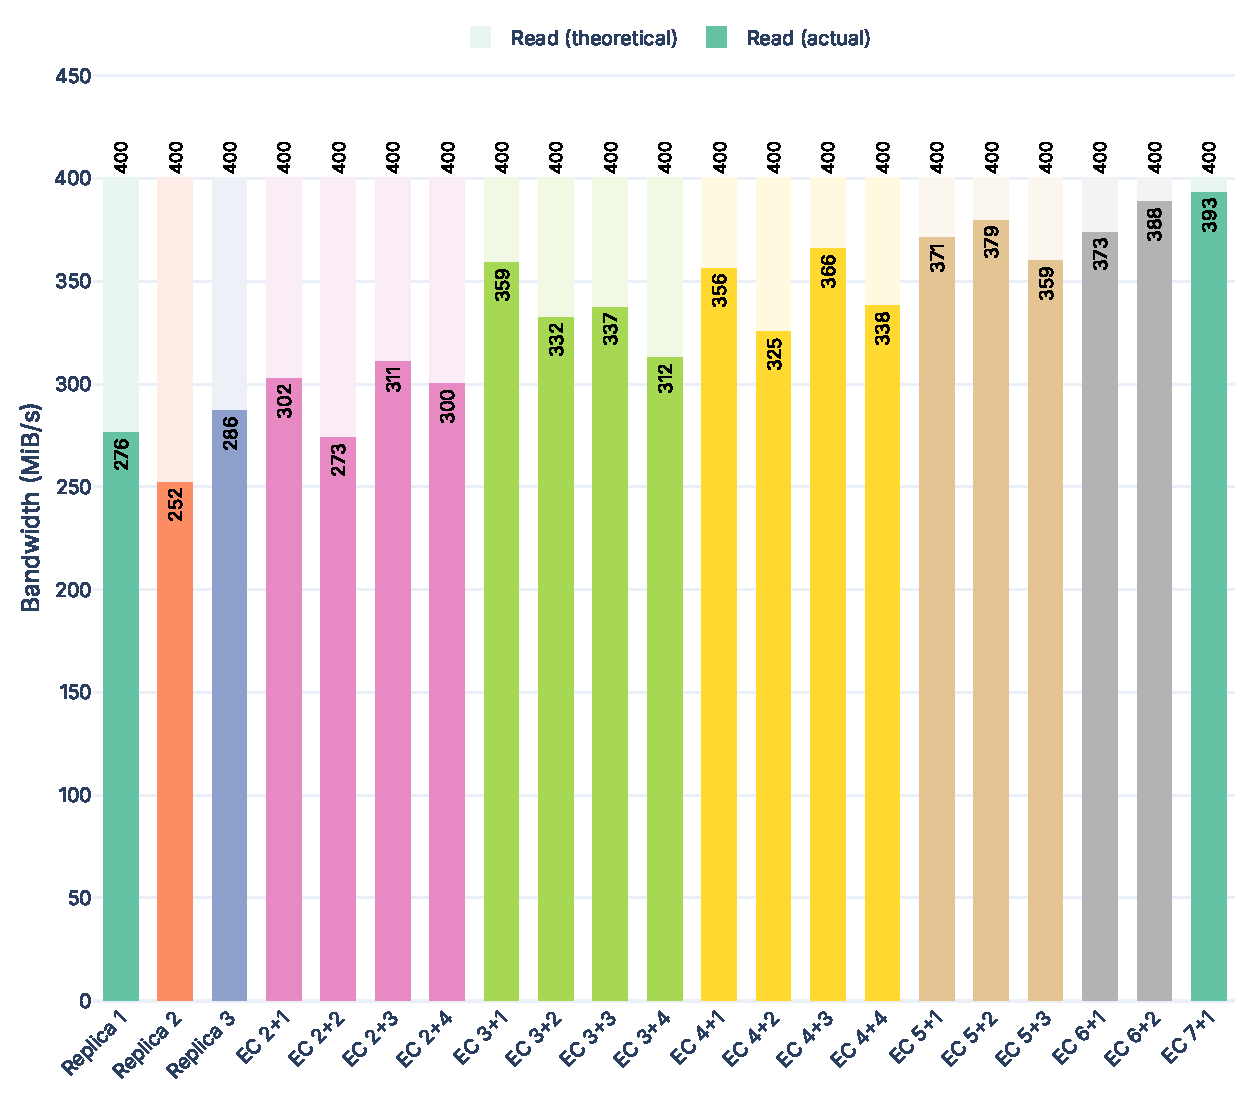
\includegraphics[width=\textwidth]{assets/perf_results/lab_128pg_read.pdf}
    \caption[128-\acs{PG} Read Performance Scaling]{Read performance scaling for 128 \acs{PG} pools with various replication and erasure coding profiles.}
    \label{fig:128pg-read-scaling}
\end{figure}

\Cref{fig:128pg-read-scaling} shows the read performance with 128 \acp{PG}. Since 128 \acp{PG} should be sufficient to distribute objects across all \acp{OSD}, the read performance should be limited by the cluster's combined throughput of 400\,MiB/s. Replication factor has no significant impact on read throughput; however, we only observed up to $\approx$ 286\,MiB/s, or 71.5\%, of the cluster's performance limit. Pools with \ac{EC} show strong performance characteristics, better than those of replicated pools, with the highest 7+1 \ac{EC} profile reaching close to the theoretical maximum.

\pagebreak
\subsubsection{128-\acs{PG} Write Performance Scaling}

\begin{figure}[H]
    \centering
    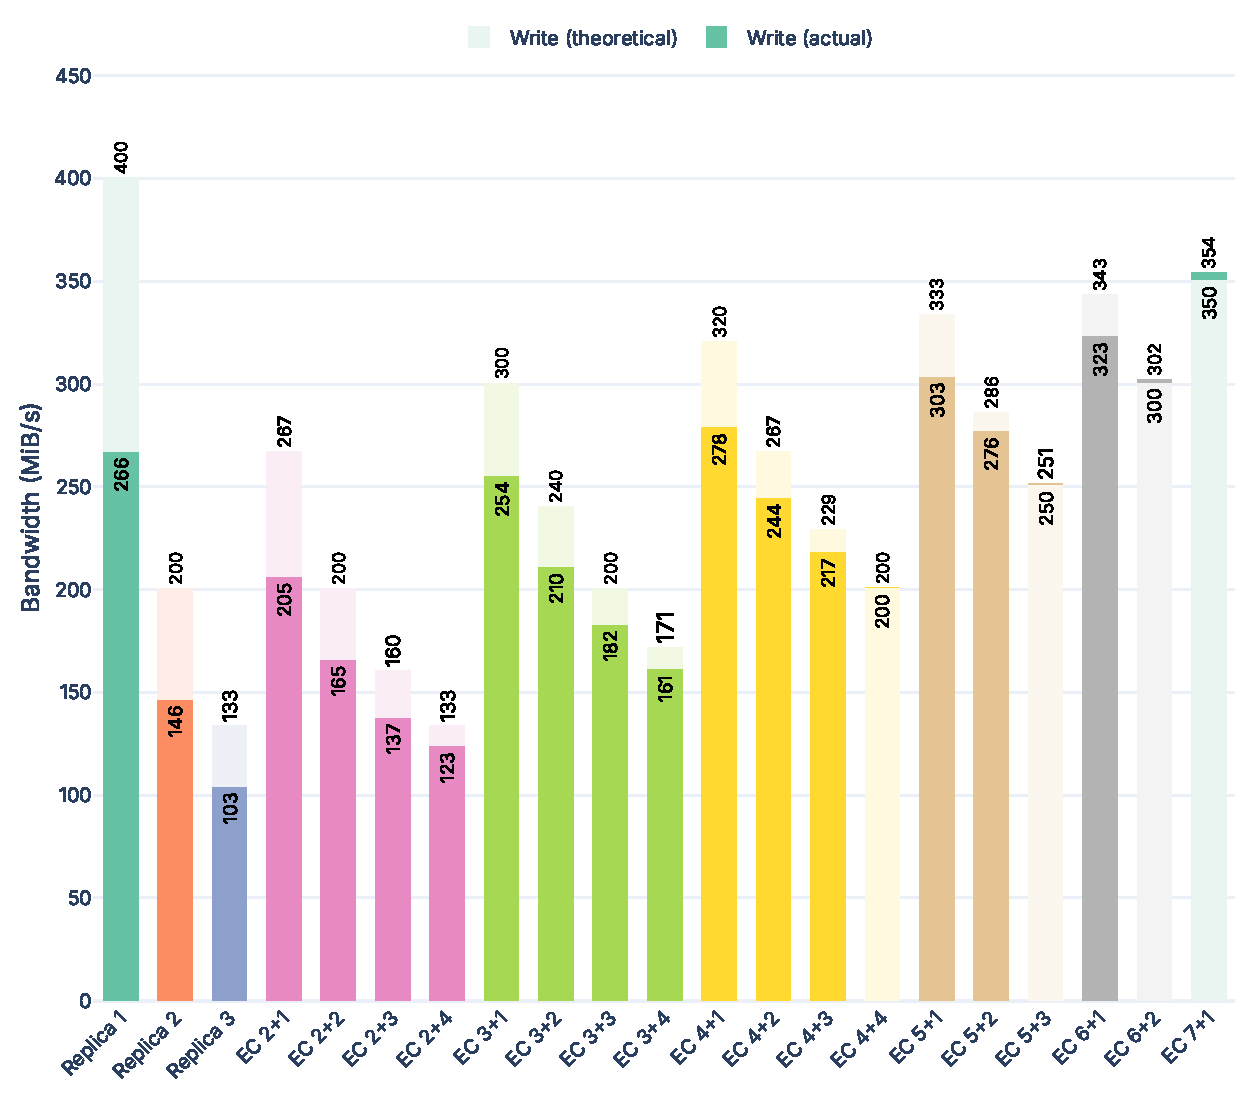
\includegraphics[width=\textwidth]{assets/perf_results/lab_128pg_write.pdf}
    \caption[128-\acs{PG} Write Performance Scaling]{Write performance scaling for 128 \acs{PG} pools with various replication and erasure coding profiles.}
    \label{fig:128pg-write-scaling}
\end{figure}

\Cref{fig:128pg-write-scaling} shows the write performance with 128 \acp{PG}. For replicated pools, the total throughput is divided by the replication factor, while for \ac{EC} pools, the write throughput is limited by the number of total coding chunks. Overall, we observed that the replicated pools achieved about 70--80\% of the block device limit, while \ac{EC} pools generally outperformed the replicated pools both in terms of efficiency and overall throughput at the same level of failure tolerance.

\pagebreak
\subsubsection{Single-\acs{PG} Read Performance Scaling}

\begin{figure}[H]
    \centering
    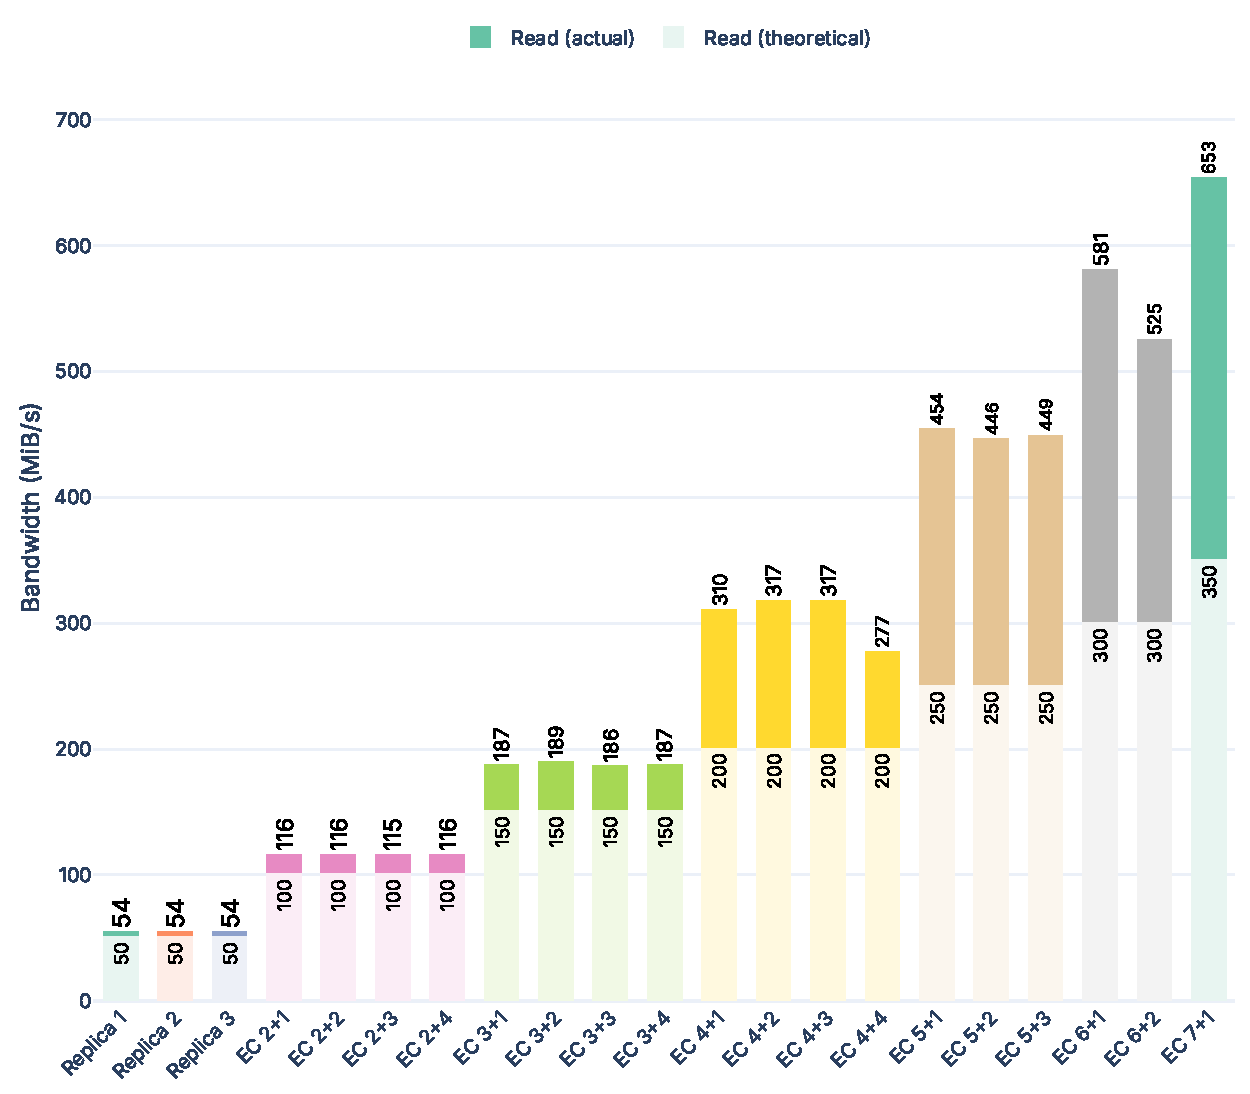
\includegraphics[width=\textwidth]{assets/perf_results/lab_1pg_read.pdf}
    \caption[Single-\acs{PG} Read Performance Scaling]{Read performance scaling for a single 
    \acs{PG} pool with various replication and erasure coding profiles.}
    \label{fig:1pg-read-scaling}
\end{figure}

\Cref{fig:1pg-read-scaling} shows read performance with a single \acs{PG}. Single-\acs{PG} pools, or single-object writes to multi-\acs{PG} pools, are a weak spot for replicated pools, as they are limited by the per-\acs{OSD} rate limit.

\subsubsection{Single-\acs{PG} Write Performance Scaling}

\begin{figure}[H]
    \centering
    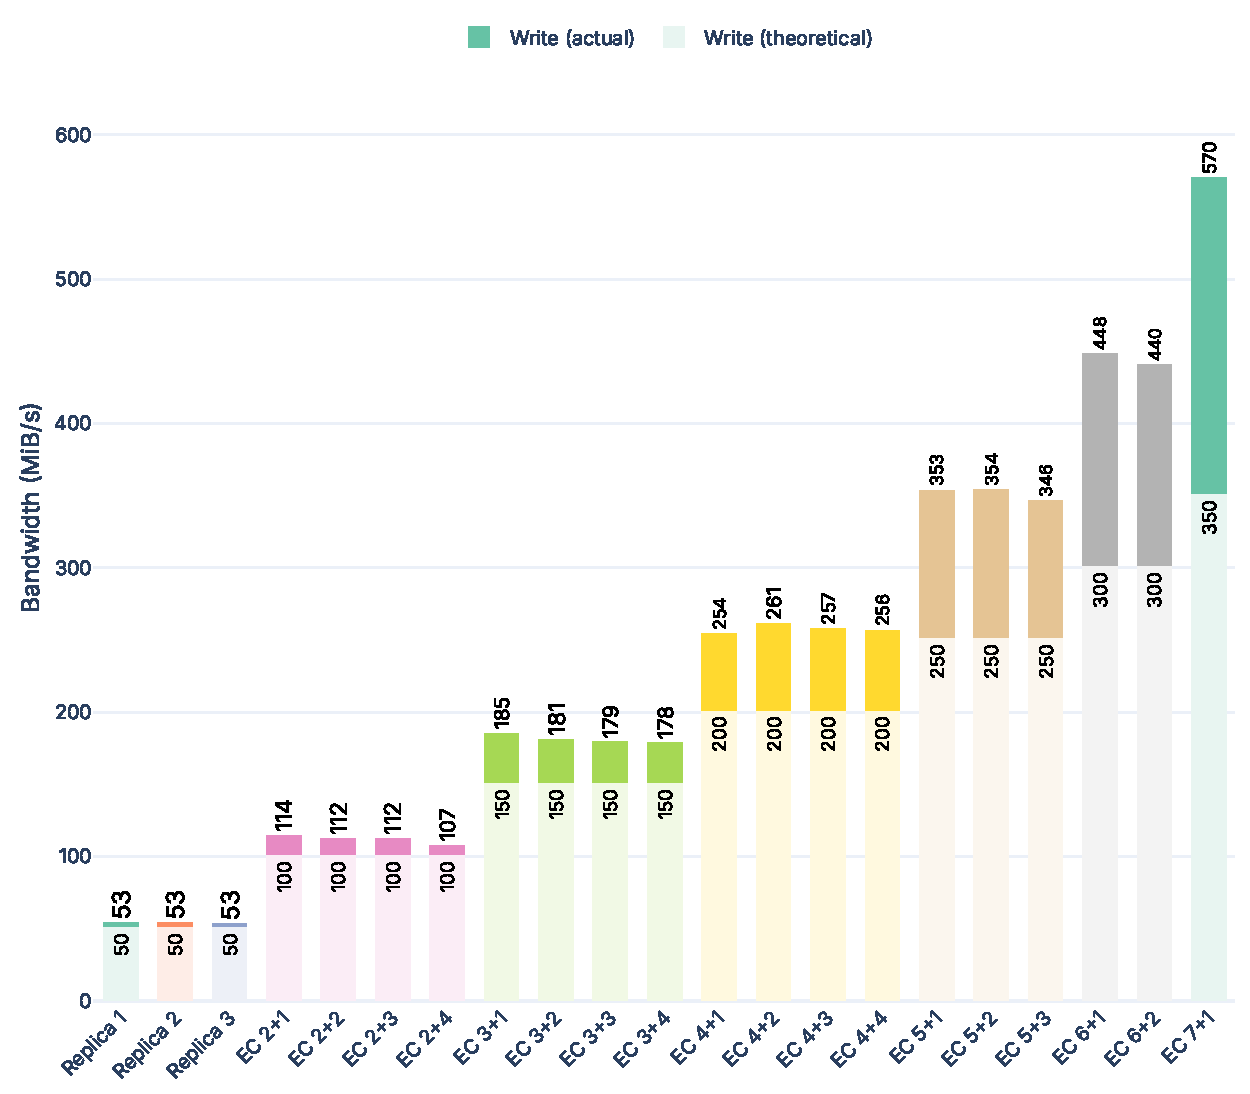
\includegraphics[width=\textwidth]{assets/perf_results/lab_1pg_write.pdf}
    \caption[Single-\acs{PG} Write Performance Scaling]{Write performance scaling for a single 
    \acs{PG} pool with various replication and erasure coding profiles.}
    \label{fig:1pg-write-scaling}
\end{figure}

\Cref{fig:1pg-write-scaling} shows write performance with a single \acs{PG}. Performance results are similar to the read performance, with replicated pools again showing flat throughput regardless of the replication factor and all pools showing higher actual performance results than the theoretical limit. As noted earlier, this is likely attributable to the burst behaviour of the throttling implementation.

\pagebreak

\subsection{Baseline Testing}
\label{sec:results-exploratory-config}

We performed initial exploratory testing with the \ac{RADOS} backend using the \ac{RDMA} and \ac{TCP} network protocols, as well as Omni-Path and InfiniBand networking, in order to determine the system and cluster configurations which were used for extended testing. Due to the time frame in which these benchmarks were run, we used Ceph v19.2.0 (Reef) instead of v20.2.0 (Tentacle) for these performance tests; the system configuration is shown in~\cref{tbl:benchmark-conditions-explore}. It is possible that newer Ceph versions may have impacted the performance results; however, the \acs{RDMA} code within Ceph has not undergone significant changes between these versions\footnote{\url{https://github.com/ceph/ceph/commits/main/src/msg/async/rdma}. Accessed 26.02.2026.}, and these results were gathered with the primary purpose of narrowing down our selection for the extended testing phase, rather than direct evaluation.

\begin{table}[H]
\centering
\begin{tabular}{|ll|}
\hline
Ceph Version       & v19.2.0 \\
Ceph Nodes         & 8 \\
Client Nodes       & 2--8 \\
Colocation         & Separate server/client nodes \\
Client Tasks       & 2--512, $1\leq t \leq 128$ per node \\
Monitors           & 1 (on node 1) \\
Managers           & 1 (on node 1) \\
\acp{OSD}          & 128 (on nodes 1--8, 16 \acp{OSD}/node) \\
\ac{OSD} size      & 12 GiB/\ac{OSD} \\
Pool Type          & Replica 3 \\
\hline
\end{tabular}
\caption[Benchmarking Conditions for Exploratory Testing]{Cluster configuration for exploratory testing.}
\label{tbl:benchmark-conditions-explore}
\end{table}

\subsubsection{Omni-Path Issues}
\label{sec:results-opa-issues}

During our initial validation runs, we were unable to collect Ceph results reliably from the nodes equipped with Omni-Path networking. The test suite was not able to complete successfully without node failures during the testing phase, which occurred on both client and cluster nodes. As a result, we have only been able to gather a limited amount of Omni-Path performance data.

\begin{figure}[H]
    \centering
    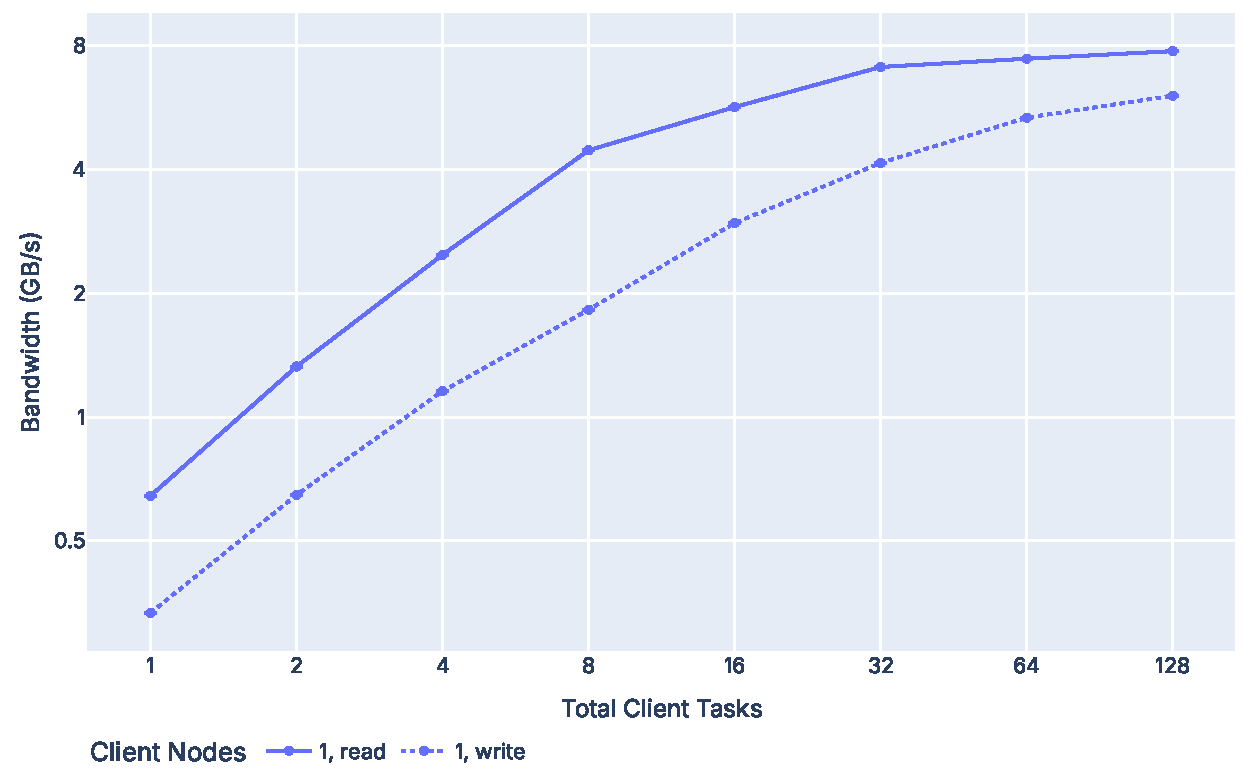
\includegraphics[width=0.9\linewidth]{assets/perf_results/omnipath_seq_64m.pdf}
    \caption[RADOS 64MiB Omni-Path Performance]{Performance results for 64MiB \acs{RADOS} read/write operations over the Omni-Path network transport.}
    \label{fig:omnipath-seq-64m}
\end{figure}

\Cref{fig:omnipath-seq-64m} shows good scaling performance results. Based on the network performance tests performed in~\cref{sec:results-network-bandwidth-opa}, peak performance is likely being limited by network performance, rather than Ceph itself.

\begin{figure}[H]
    \centering
    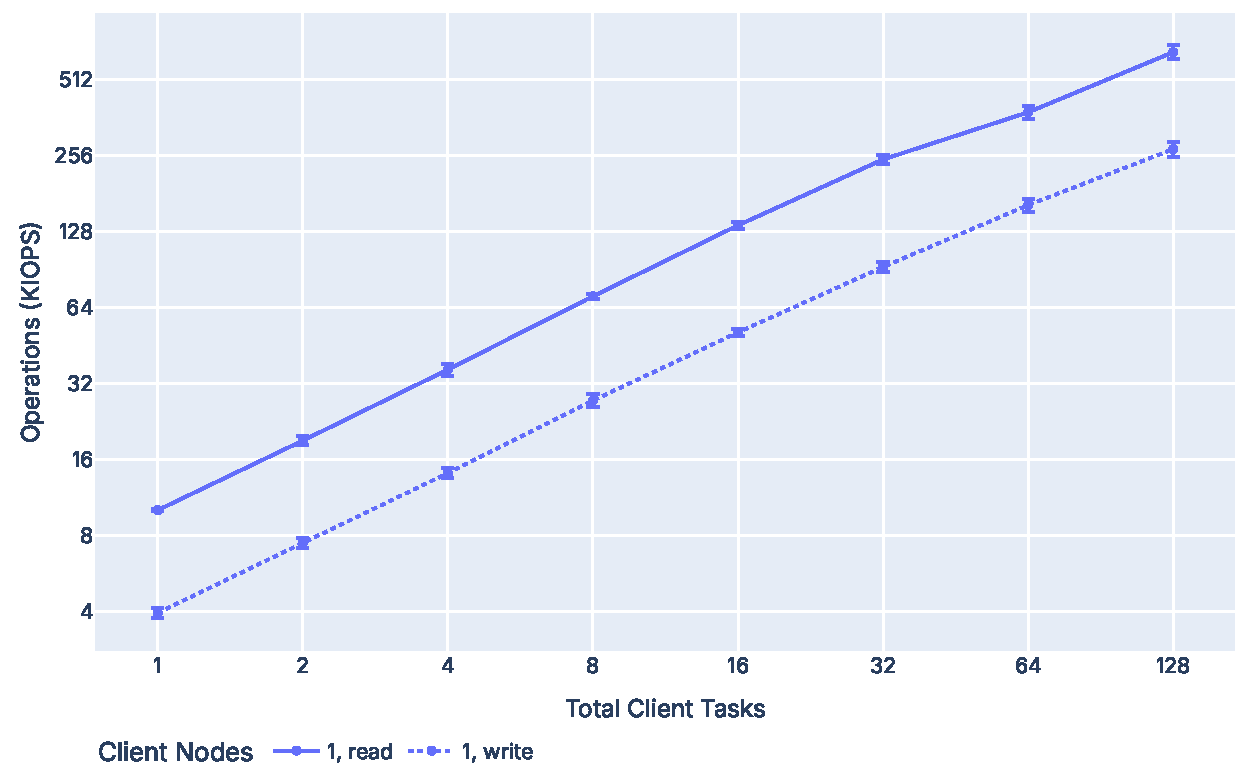
\includegraphics[width=0.9\linewidth]{assets/perf_results/omnipath_4k_iops.pdf}
    \caption[RADOS 4KiB Omni-Path Performance]{Performance results for 4KiB \acs{RADOS} read/write operations on 2MiB objects over the Omni-Path network transport.}
    \label{fig:omnipath-seq-4k}
\end{figure}

\Cref{fig:omnipath-seq-4k} demonstrates close to linear scaling for 4KiB read and write operations, suggesting a performance bottleneck primarily on the client side.

The partial performance results suggest that Omni-Path could be a suitable network platform for Ceph. However, the node failures effectively made Ceph unusable on the Omni-Path platform. Therefore, we investigated the source of the issue further.

\subsubsection{Root Cause Analysis for Omni-Path Kernel Panics}
\label{sec:opa-bad-root-cause-analysis}

Following discussions with system administrators, it was confirmed that the affected nodes could only be reached through their out-of-band management interfaces. This ruled out possible firewall restrictions or rate limits, which were not in place for such traffic. These causes were therefore excluded from consideration.

To rule out hardware defects, additional experiments were performed on the nodes within the same cluster partition (medium96s). These nodes exhibited identical failures to those initially observed. The standard96 partition was also tested: this partition contains a different hardware configuration, as shown in~\cref{tbl:standard96-system}.

\begin{table}[H]
\centering
\begin{tabular}{|ll|}
\hline
\textbf{Component} & \textbf{Specification} \\
\hline
CPU        & 2$\times$ Intel Xeon Platinum 9242 (48C/96T per CPU) \\
RAM        & 384 GB \\
Networking & 100 Gbps Omni-Path (Intel HFI100) \\
\hline
\end{tabular}
\caption[Omni-Path Failure Test Hardware]{The hardware configuration of the second cluster partition \texttt{standard96}, used to reproduce the Omni-Path kernel panic issue and exclude issues specific to the \texttt{medium96s} partition.}
\label{tbl:standard96-system}
\end{table}

Node failures persisted under this configuration. Based on this information, the causes were narrowed down to a possible issue with the software stack or the Omni-Path networking itself, rather than other hardware-specific issues.

After exclusion of these factors, the hypothesis was that the kernel, or possibly some other element in the software stack, was failing, leading to
system instability. 
In order to test this hypothesis, kernel logs were collected during benchmark execution. 
This task was made somewhat more complex due to the cluster nodes' boot method; nodes boot from the network and copy the image contents into a volatile file system (tmpfs) stored in-memory\footref{appendix:tmpfs-in-memory}. 
Any collected logs would therefore be lost on node failure or reboot, and no elevated privileges were available to change this behaviour\footref{appendix:dmesg-unprivileged}. 
As a workaround to this limitation, two methods were employed in an attempt to stream kernel logs gathered via the \texttt{dmesg -w} command prior to system failure, namely writing kernel logs to a local disk mounted at \texttt{/local}, and streaming kernel output via the network to a separate node not part of the Ceph cluster.

As a result of the kernel panic causing system halts, some failures did not write usable logs, either to the disk or via the network. 
Ultimately, after several attempts, a single useful log was recovered from a failed system via the network, via the node's secondary Ethernet network interface. The relevant sections of the collected logs are shown in \Cref{lst:opa-crash}.

\pagebreak
\lstinputlisting[
    caption={
        [Omni-Path Related Kernel Panic]
        Omni-Path related kernel panic. The source of the kernel panic is an invalid pointer access in the \texttt{hfi1\_ipoib\_send\_dma\_common} function, triggered by \ac{TCP} network activity from the
        Ceph traffic.
    },
    label={lst:opa-crash},
    frame=single,
    breaklines=true
]{assets/network/opa_crash.txt}

Searching for this specific cause, \texttt{hfi1\_ipoib\_send\_dma\_common},
leads to a report of a vulnerability (CVE-2024-26766). At the time, however, the \ac{RHEL} 8
kernel on which Rocky Linux 8 is based was reported as not affected by the
vulnerability.

Based on the bug description, we attempted to reproduce the issue in order to narrow down this issue as a possible cause of the node failures by constructing a proof-of-concept to generate an unaligned message with the correct number of \ac{SDMA} descriptors. An upstream \ac{RHEL} 8 installation was used, installed on the Omni-Path performance testing system previously detailed in~\cref{tbl:validation-system} to verify the bug stems from the upstream kernel.

\pagebreak
\lstinputlisting[
    caption={
        [Kernel Panic with Reproducer \acs{PoC}]
        Kernel panic triggered by the reproducer proof-of-concept code.
    },
    label={lst:opa-crash-poc-dmesg},
    frame=single,
    breaklines=true
]{assets/network/bug/crash-ryzen.txt}

Running the reproducer code reliably triggered the kernel panic as shown in~\cref{lst:opa-crash-poc-dmesg}; however, the exact location of the kernel panic was different to that of the Ceph-traffic-induced panic. Running this code on the same system with \ac{RHEL} 9 installed did not result in a kernel panic.

As the issue could successfully be reproduced, and because the issue represents a moderate security vulnerability of the \ac{RHEL} kernel itself rather than issues specific to our testing, the \ac{PoC} and associated report details were submitted to Red Hat privately for resolution. The vulnerability status was acknowledged and updated by Red Hat, and a security patch was released by Red Hat on 02.02.2026\footnote{\url{https://access.redhat.com/errata/RHSA-2026:1662}. Accessed 02.02.2026.}. As of 15.02.2026, the fixed kernel version (4.18.0-553.100.1.el8\_10) is provided by Rocky Linux\footnote{Kernel updates were checked on a Rocky Linux 8.10 installation.}. However, due to time constraints, it was not possible to perform additional Ceph performance testing on the Omni-Path network transport. Additionally, at the time of writing, the cluster kernel was not yet updated to this patched version. However, a manually patched \texttt{hfi1} kernel module applying the fixes for the vulnerability was successfully tested on a single node with root access provided by the cluster administrators.

\subsubsection{Transport Comparison}
\label{sec:transport-comparison-rados}

Due to the issues detailed in~\cref{sec:results-opa-issues}, we performed further performance benchmarks of the \ac{RDMA}/\ac{TCP} transport only on the InfiniBand-equipped nodes. It should be noted that, as we described in~\cref{sec:results-exploratory-config}, \ac{RDMA} performance benchmarks were performed using Ceph v19.2.0 (Reef), rather than v20.2.0 (Tentacle) used in the remainder of this evaluation.

\subsubsection*{Large Object Operations}

\begin{figure}[H]
    \centering
    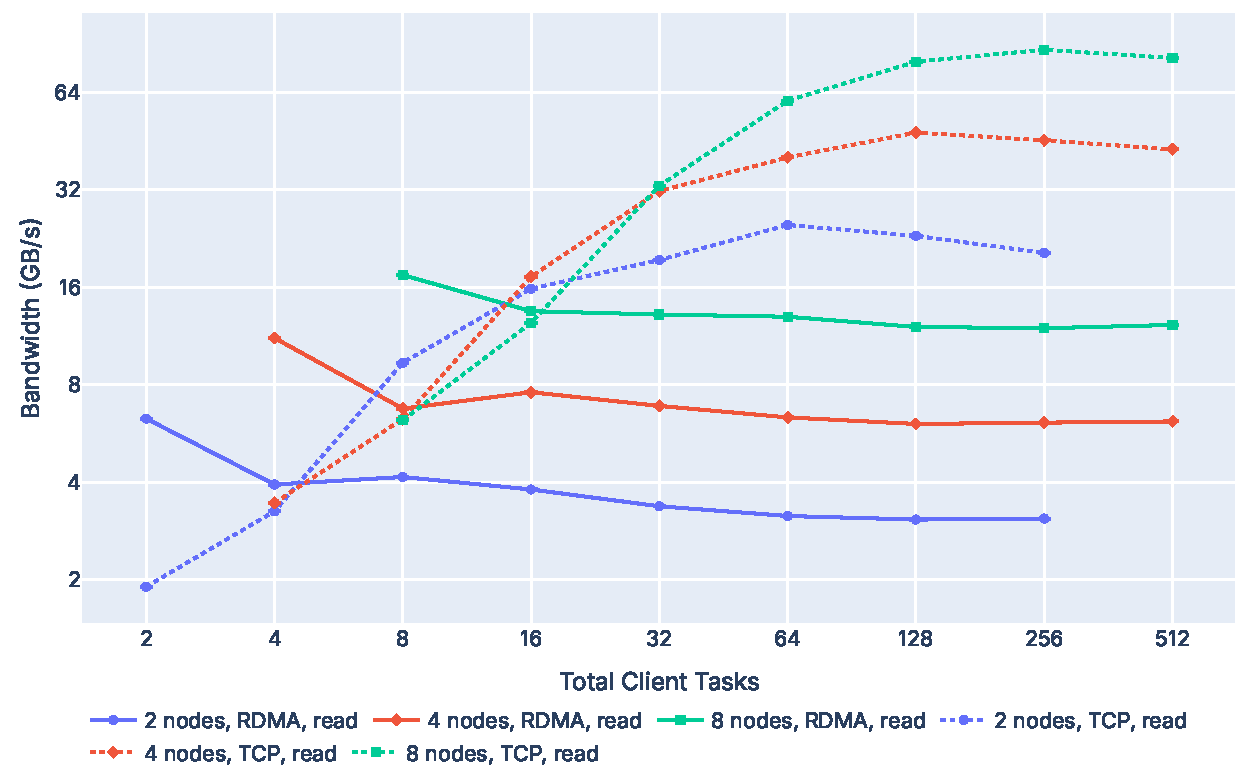
\includegraphics[width=0.9\linewidth]{assets/perf_results/rados_rdma_vs_tcp_seq_64m_read.pdf}
    \caption[RADOS RDMA/TCP Sequential Read Performance Comparison]{Comparison of 64MiB \acs{RADOS} reads using \acs{RDMA} and \acs{TCP} as the messenger backends.}
    \label{fig:rados-rdma-vs-tcp-seq-64m-read}
\end{figure}

\begin{figure}[H]
    \centering
    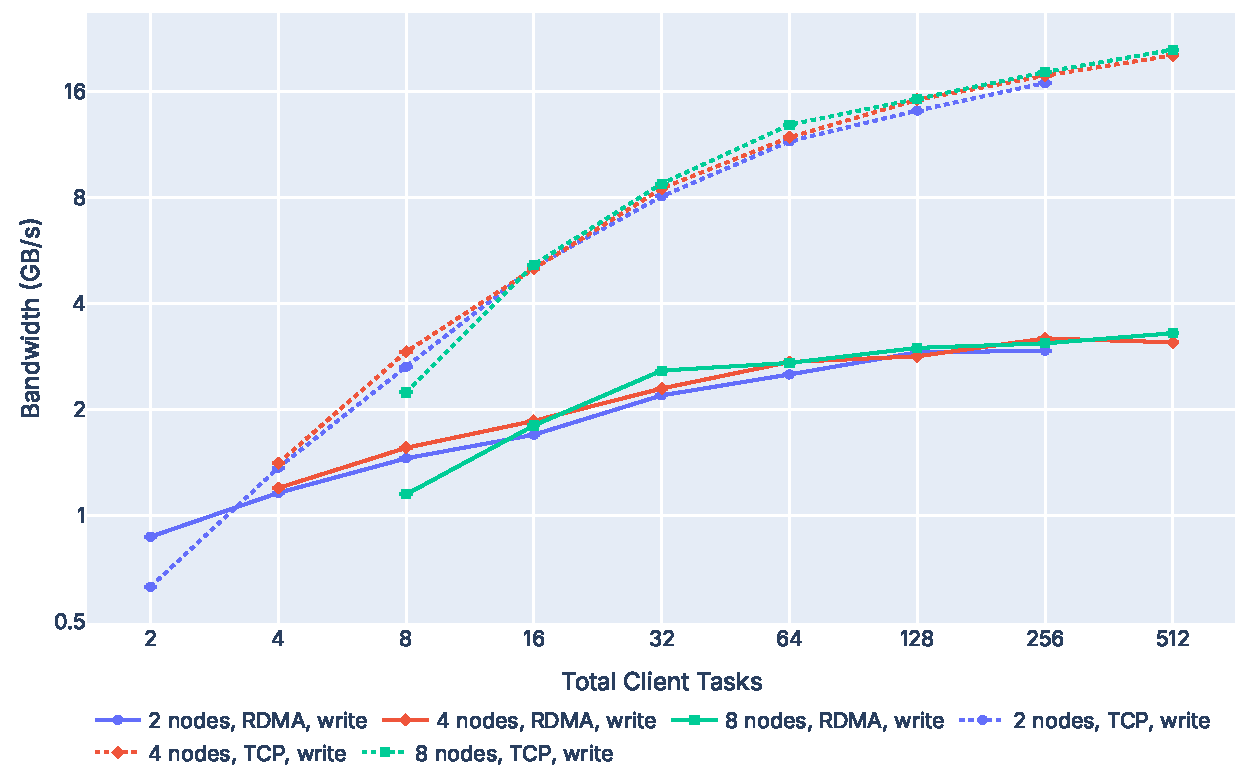
\includegraphics[width=0.9\linewidth]{assets/perf_results/rados_rdma_vs_tcp_seq_64m_write.pdf}
    \caption[RADOS RDMA/TCP Sequential Write Performance Comparison]{Comparison of 64MiB \acs{RADOS} writes using \acs{RDMA} and \acs{TCP} as the messenger backends.}
    \label{fig:rados-rdma-vs-tcp-seq-64m-write}
\end{figure}

\Cref{fig:rados-rdma-vs-tcp-seq-64m-read} demonstrates the unusual performance observed when using \ac{RDMA} as the messenger transport. Unlike \ac{TCP}, throughput scaling was not observed with increased task counts; performance immediately reached a per-node performance limitation. This resulted in performance at low numbers of tasks per node being $\approx3\times$ higher with \ac{RDMA} over \ac{TCP}, yet significantly lower at high task counts---\ac{TCP} performance was $\approx7\times$ higher than \ac{RDMA} at the maximum number of tasks per node.

\Cref{fig:rados-rdma-vs-tcp-seq-64m-write} additionally demonstrates poor write performance; regardless of the node count, write performance at the same number of tasks per node is nearly identical and generally significantly worse than that of \ac{TCP}, with the only exception being the performance at 2 total tasks. At the maximum task count, \ac{TCP} performance exceeded \ac{RDMA} performance by a factor of 6.5.

\subsubsection*{Small Object Operations}

\begin{figure}[H]
    \centering
    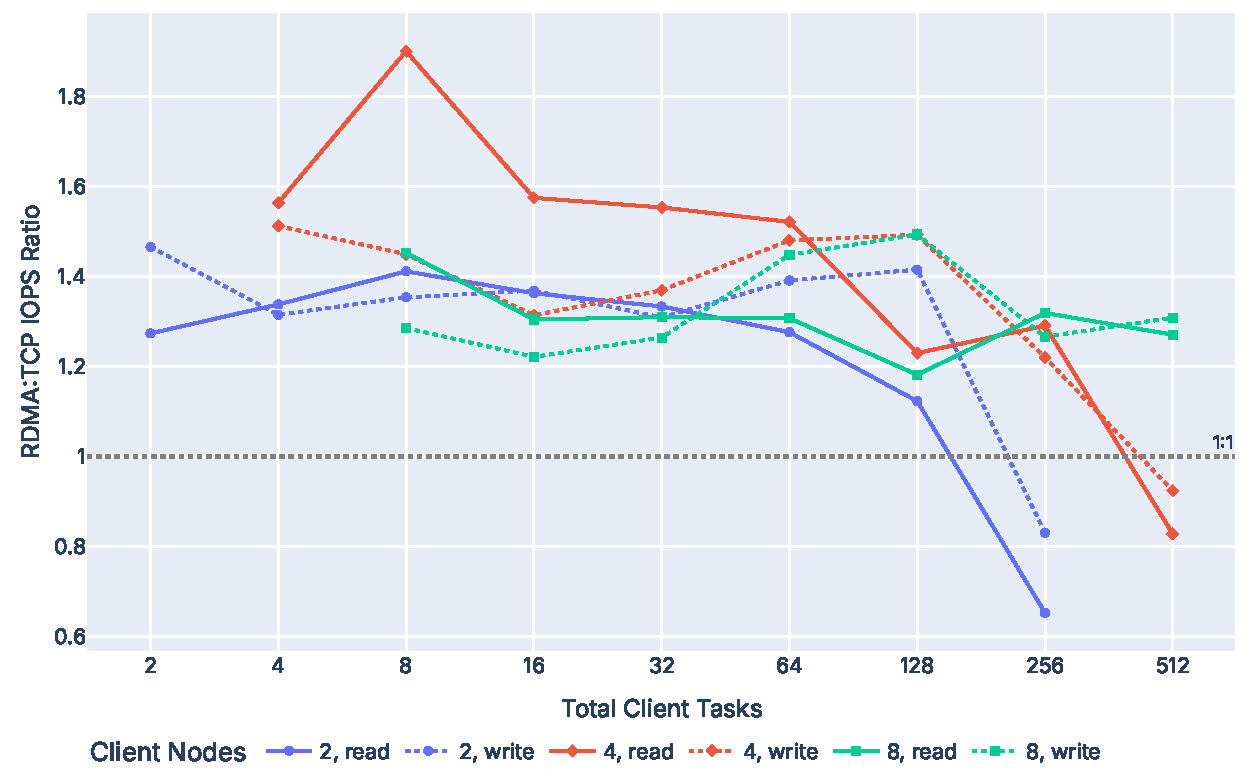
\includegraphics[width=0.9\linewidth]{assets/perf_results/rados_rdma_tcp_ratio_4k.pdf}
    \caption[RADOS RDMA/TCP 4KiB Write Performance Comparison]{Performance comparison between \acs{RDMA} and \acs{TCP} for 4KiB \ac{RADOS} operations.}
    \label{fig:rados-rdma-tcp-ratio-4k}
\end{figure}

\Cref{fig:rados-rdma-tcp-ratio-4k} shows that the performance of the \ac{RDMA} transport for small writes is modestly higher for most combinations of nodes and client tasks. In addition, although the performance at 2 nodes/256 tasks and 4 nodes/512 tasks is lower than that of the \ac{TCP} transport, the performance penalty is much less significant than for large read/write sizes; the lowest relative performance result shows \ac{TCP} outperforming \ac{RDMA} by a factor of 1.5, rather than the 6.5--7$\times$ observed in the large \ac{I/O} performance results.

\subsubsection{Additional Issues}

In addition to these performance issues, we also observed sporadic failures for the \ac{IOR} benchmark to complete at high task counts, with disconnection issues being shown only in Ceph logs, as shown in~\cref{lst:ceph-ib-full}. Due to stability issues with the \ac{RDMA} transport, we also could not perform additional \ac{CephFS} performance testing.

\lstinputlisting[
    language=ini,
    caption={Ceph InfiniBand Connection Dropout Messages},
    label={lst:ceph-ib-full},
    frame=single,
    breaklines=true,
    float
]{assets/ceph/infiniband_conn_drop.txt}

%%%%%%%%%%%%%%%%%%%%%%%%%%%%%%%%%%%%%%%%%%%%%%%%%%%%%%%%%%%%%%%%%%%%%%%%%%%%%%%%%%%%%%%%%%%%%%%%

\pagebreak
\subsection{Benchmark Configuration}

The system configuration for the benchmarks performed is shown in~\cref{tbl:benchmark-conditions}. Benchmarks where InfiniBand networking was used have the configuration as shown in~\cref{tbl:infiniband-system}, while Omni-Path nodes are configured as in~\cref{tbl:omnipath-system}. Due to the performance and stability issues observed in~\cref{sec:transport-comparison-rados}, \ac{TCP} was used for all of the following benchmarks.

\begin{table}[h]
\centering
\begin{tabular}{|ll|}
\hline
Ceph Nodes         & 7 \\
Client Nodes       & 2--8 \\
Colocation         & Separate server/client nodes \\
Client Tasks       & 2--512, $1\leq t \leq 128$ per node \\
Monitors           & 1 (on node 1) \\
Managers           & 1 (on node 1) \\
\acp{OSD}          & 48 (on nodes 2--7, 8 \acp{OSD}/node) \\
\ac{OSD} size      & 24 GiB/\ac{OSD} \\
\acp{MDS}          & 4 (on node 1) \\
Replicated Pool Type & Replica 3 \\
\multirow{2}{*}{Erasure-Coded Pool Type} & 4+2 (\acs{RADOS}/\acs{CephFS} data pool) \\
& Replica 3 (\acs{CephFS} metadata pool) \\
\hline
\end{tabular}
\caption{Benchmarking Conditions}
\label{tbl:benchmark-conditions}
\end{table}

\subsection{Large Sequential \acs{I/O} Operations}

In order to evaluate sequential \ac{I/O} performance, we used the \ac{IOR} benchmark with various configurations. The replicated configuration used a data pool with replica 3; for \ac{CephFS}, a secondary metadata pool with replica 3 was also created. The erasure coding configuration used 4 data chunks and 2 coding chunks for the data pool; however, the \ac{CephFS} metadata pool remains as replica 3, as replicated metadata pools are required for \ac{CephFS}.

\subsubsection{\acs{RADOS} -- Replicated}

For large \ac{I/O} operation tests, we used individual objects/files, each 64 MiB in size. Larger objects caused issues with the \ac{RADOS} backend due to its default size limit of 128 MiB. Adjusting the maximum object size is possible, however, this option is discouraged by Ceph for practicality reasons\footnote{\url{https://ceph.io/en/news/blog/2017/v12-1-4-luminous-rc-released/}. Accessed 23.02.2026.}.

\begin{figure}[H]
    \centering
    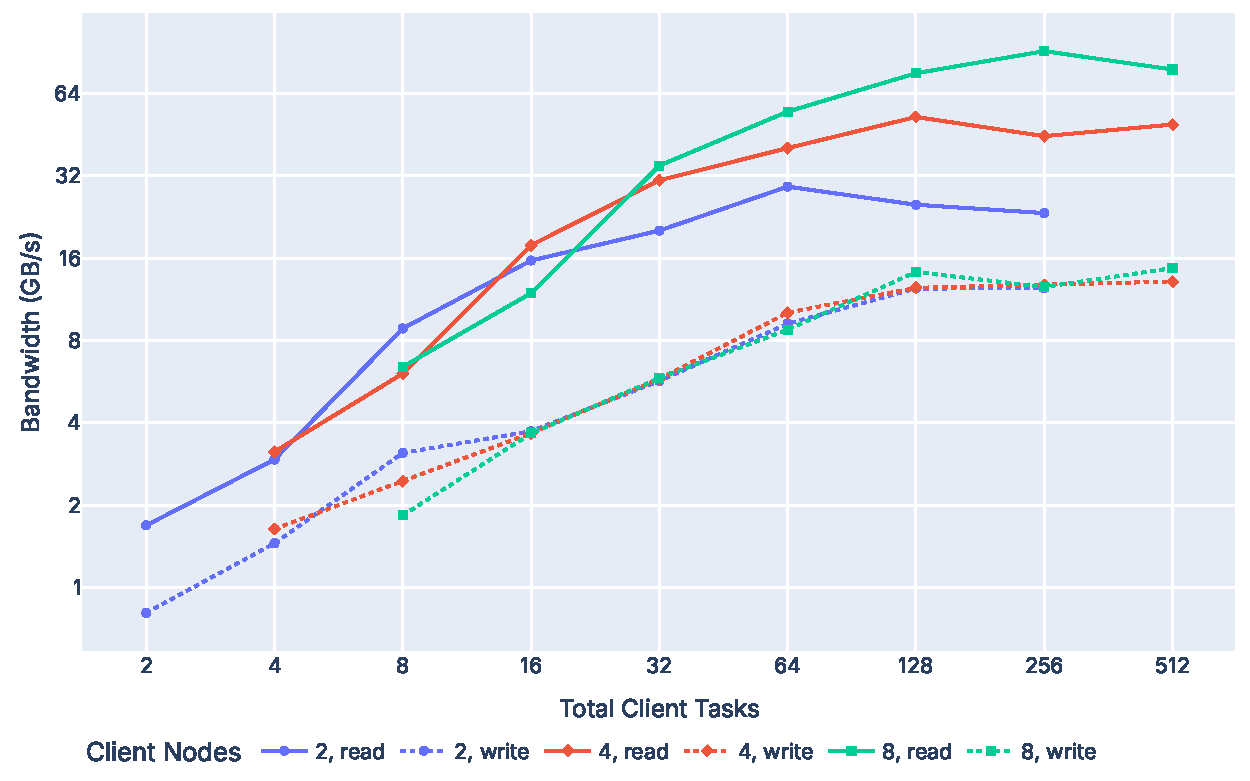
\includegraphics[width=\linewidth]{assets/perf_results/rados_tcp_seq_64m_repl3.pdf}
    \caption[RADOS 64MiB Sequential Read/Write I/O Performance]{Sequential read/write I/O performance using the \acs{RADOS} interface demonstrating scaling performance.}
    \label{fig:rados-tcp-seq-64m-repl3}
\end{figure}

\begin{figure}[H]
    \centering
    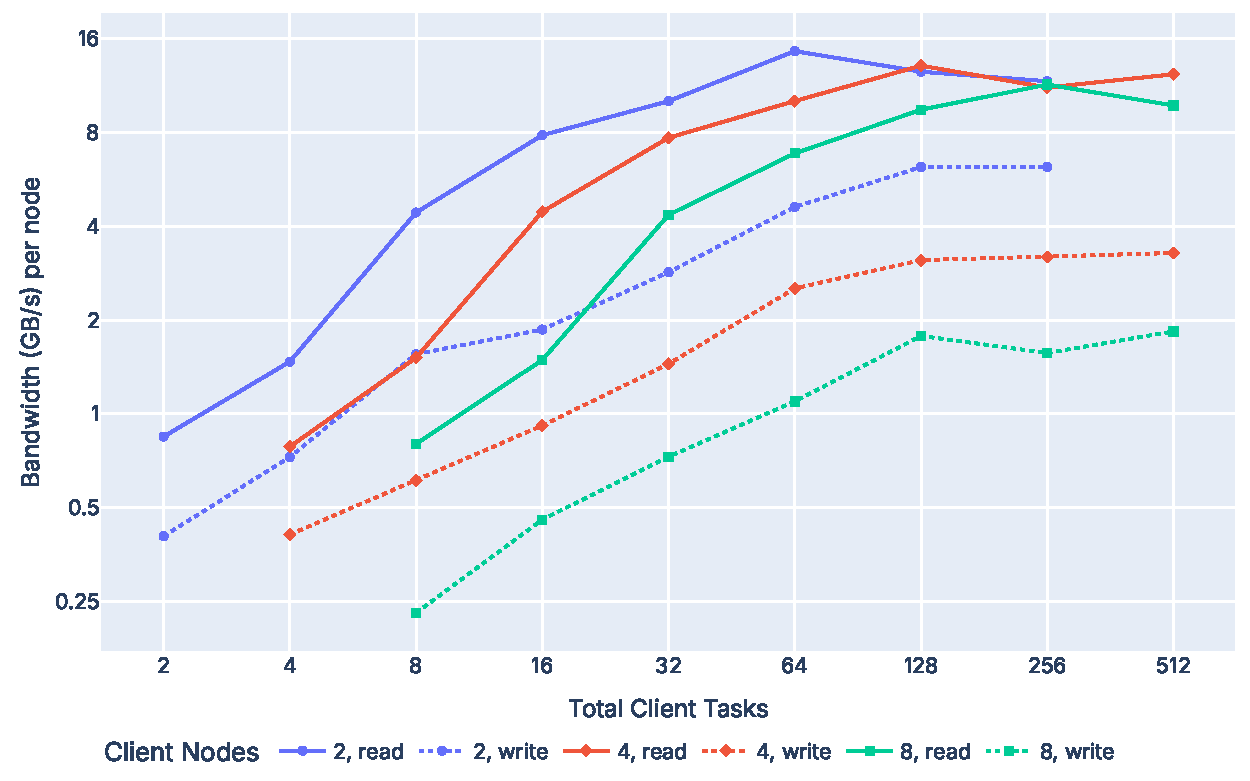
\includegraphics[width=\linewidth]{assets/perf_results/rados_tcp_seq_64m_repl3_pernode_normalized.pdf}
    \caption[RADOS 64MiB Sequential Read/Write I/O Performance (Normalized)]{Normalized sequential read I/O performance using the \acs{RADOS} interface showing per-node scaling limitations.}
    \label{fig:rados-tcp-seq-64m-repl3-pernode-normalized}
\end{figure}

\Cref{fig:rados-tcp-seq-64m-repl3} demonstrates the sequential \ac{I/O} performance with the \ac{RADOS} backend, showing strong scaling performance on reads limited primarily by per-node throughput. Normalizing the results as shown in \Cref{fig:rados-tcp-seq-64m-repl3-pernode-normalized} such that the Y-axis shows the total bandwidth per node, we can see near-linear scaling with the number of tasks per node up to a performance ceiling slightly over 100\ Gbit/s. This suggests that given a sufficient number of nodes, it is possible for Ceph to scale up further in terms of read performance. However, write performance is bottlenecked with an overall limit of 10--15 GB/s, regardless of the number of client nodes.

\begin{figure}[H]
    \centering
    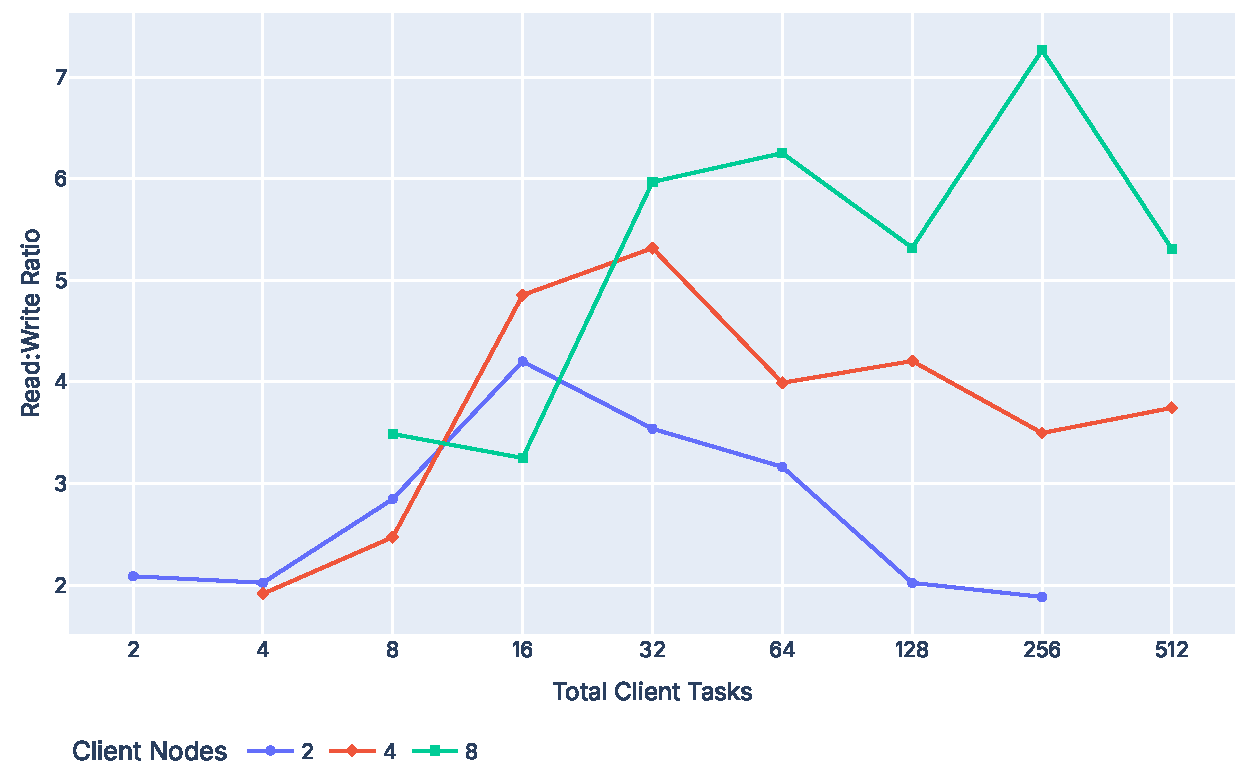
\includegraphics[width=\linewidth]{assets/perf_results/rados_tcp_seq_64m_repl3_wr_ratio.pdf}    
    \caption[RADOS 64MiB Sequential Read-Write Ratio]{\acs{I/O} performance ratio (read:write) demonstrating significant write overhead.}
    \label{fig:rados-tcp-seq-64m-repl3-wr-ratio}
\end{figure}

Write performance is limited to 10--15 GiB/s overall, regardless of the node count, which suggests a cluster-side limitation. Given that the cluster is set up in a replica-3 configuration, we expect that the read:write performance ratio would be approximately 3:1 in \acs{OSD}-performance-limited conditions. Due to the way in which Ceph performs replicated writes---the write is performed once by the client to the primary \ac{OSD}, which replicates it to the other \acp{OSD} in the group---network performance limitations are more likely to be a result of cluster-side bottlenecks. This is especially the case for our test cluster, as both the client and Ceph cluster nodes have identical hardware configurations. The actual read:write performance ratio, shown in~\cref{fig:rados-tcp-seq-64m-repl3-wr-ratio}, shows a much higher write performance penalty, especially at higher node counts when the system runs into the cluster-wide write performance bottlenecks. The read:write performance ratio does not fall below 2:1.

\subsubsection{\acs{RADOS} -- Erasure Coding}

\begin{figure}[H]
    \centering
    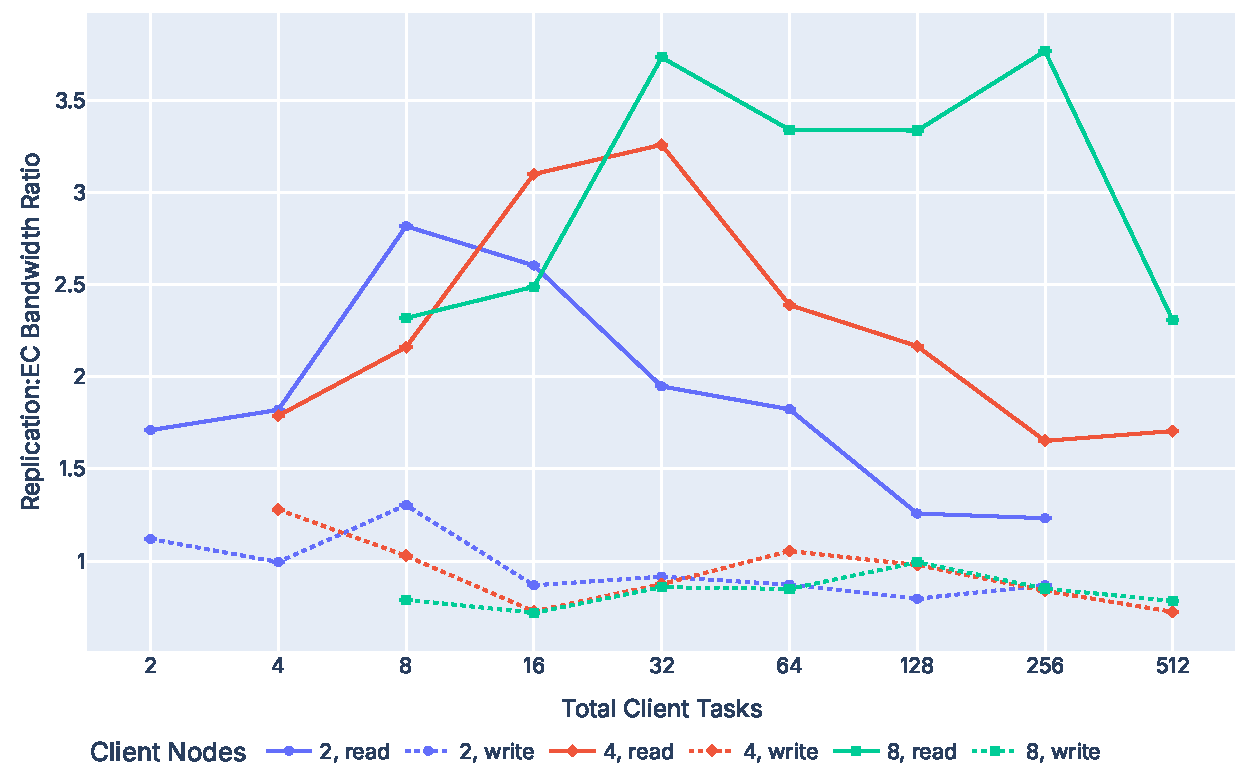
\includegraphics[width=\linewidth]{assets/perf_results/rados_tcp_repl_ec_ratio_seq_64m.pdf}
    \caption[\acs{RADOS} Erasure-Coding 64MiB Sequential Read/Write I/O Performance]{Sequential read/write \ac{I/O} performance of the \ac{RADOS} layer of replica-3 vs. 4+2 erasure-coding (EC) pools, demonstrating the performance impacts of erasure coding.}
    \label{fig:rados-tcp-repl-ec-ratio-seq-64m}
\end{figure}

\Cref{fig:rados-tcp-repl-ec-ratio-seq-64m} demonstrates the 4+2 erasure-coded read performance compared to replicated pools. In this configuration, a single object read results in the reading of data striped across all \acp{OSD}---since the \acp{OSD} are not bottlenecked by the underlying storage, \ac{EC} reads perform worse than standard replication. However, write performance behaviour with \ac{EC} is similar to that of replication, showing near-identical scaling. Overall, we observed that \ac{EC} writes at high client counts tended to perform better than replicated writes: this could be a result of the implicit striping performed by \ac{EC} across multiple \acp{OSD} reducing the overall write load on a single \ac{OSD}.

\pagebreak
\subsubsection{\acs{CephFS} -- Replicated}

\begin{figure}[H]
    \centering
    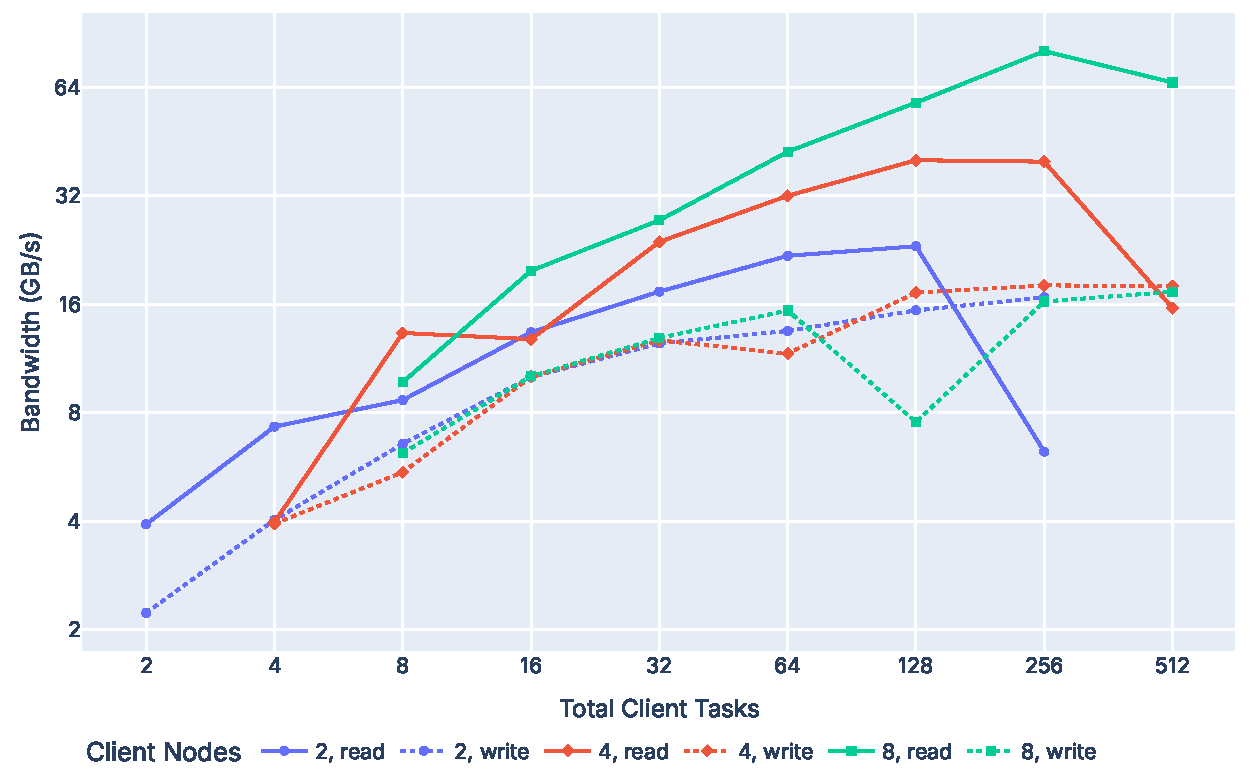
\includegraphics[width=0.9\linewidth]{assets/perf_results/cephfs_tcp_seq_64m_repl3.pdf}
    \caption[\acs{CephFS} 64MiB Sequential Read/Write I/O Performance]{Sequential read/write I/O performance using the \acs{CephFS} interface demonstrating scaling performance.}
    \label{fig:cephfs-tcp-seq-64m-repl3}
\end{figure}

\begin{figure}[H]
    \centering
    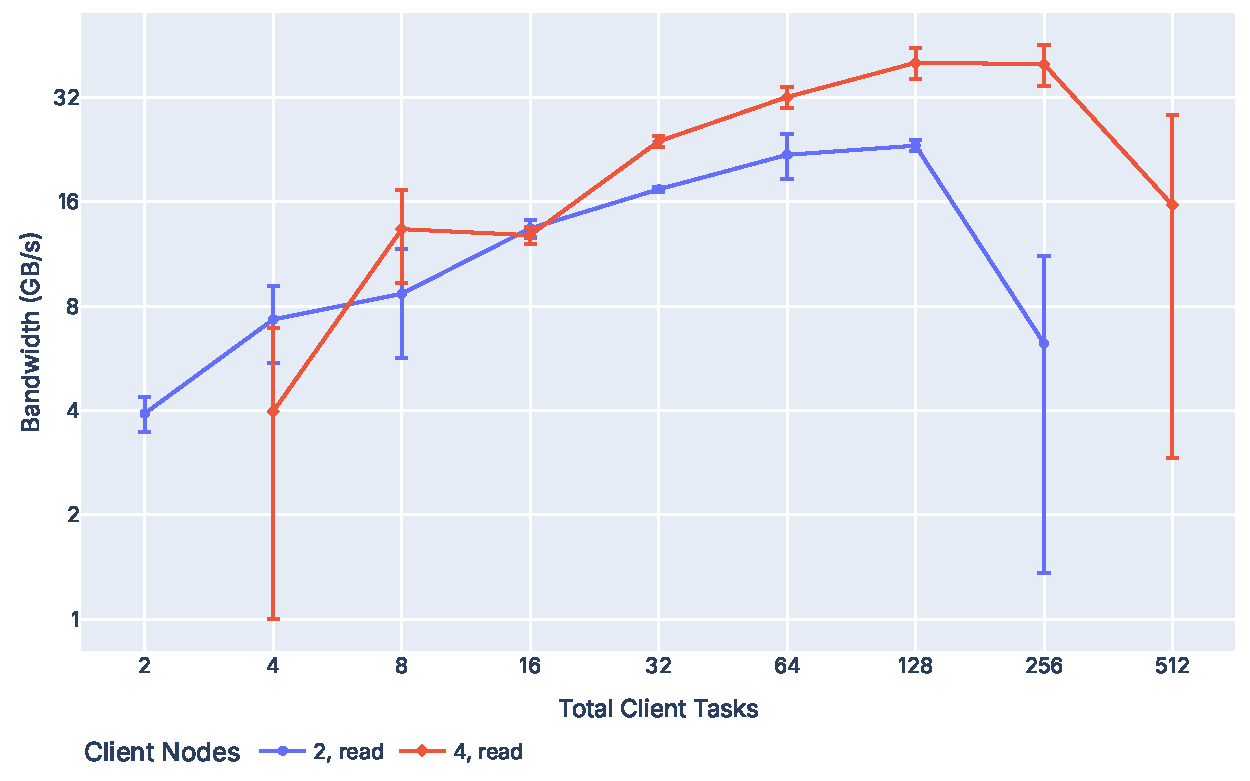
\includegraphics[width=0.9\linewidth]{assets/perf_results/cephfs_tcp_seq_64m_repl3_selected_error.pdf}
    \caption[\acs{CephFS} 64MiB Sequential Read/Write I/O Performance Variance]{Selected read performance plots of the \acs{CephFS} backend, showing unstable performance.}
    \label{fig:cephfs-tcp-seq-64m-repl3-selected-error}
\end{figure}

\Cref{fig:cephfs-tcp-seq-64m-repl3} shows similar sequential \ac{I/O} performance and scaling behaviour to that of the \ac{RADOS} backend, with the exception of an increased number of outliers, such as the performance drop in read performance for the tests involving 2 nodes/256 tasks and 4 nodes/512 tasks. Isolating these traces in~\cref{fig:cephfs-tcp-seq-64m-repl3-selected-error} shows very high performance variations for the outliers. Given that both of these tasks are using all available cores on the client nodes, this could be a result of \ac{CPU} time contention on the client side rather than performance bottlenecks on the cluster side. It is possible that the \ac{CephFS} layer, being more complex, is more \ac{CPU}-intensive than the \ac{RADOS} layer, leading to \ac{CPU} contention.

\subsubsection{\acs{CephFS} -- Erasure Coding}

\begin{figure}[H]
    \centering
    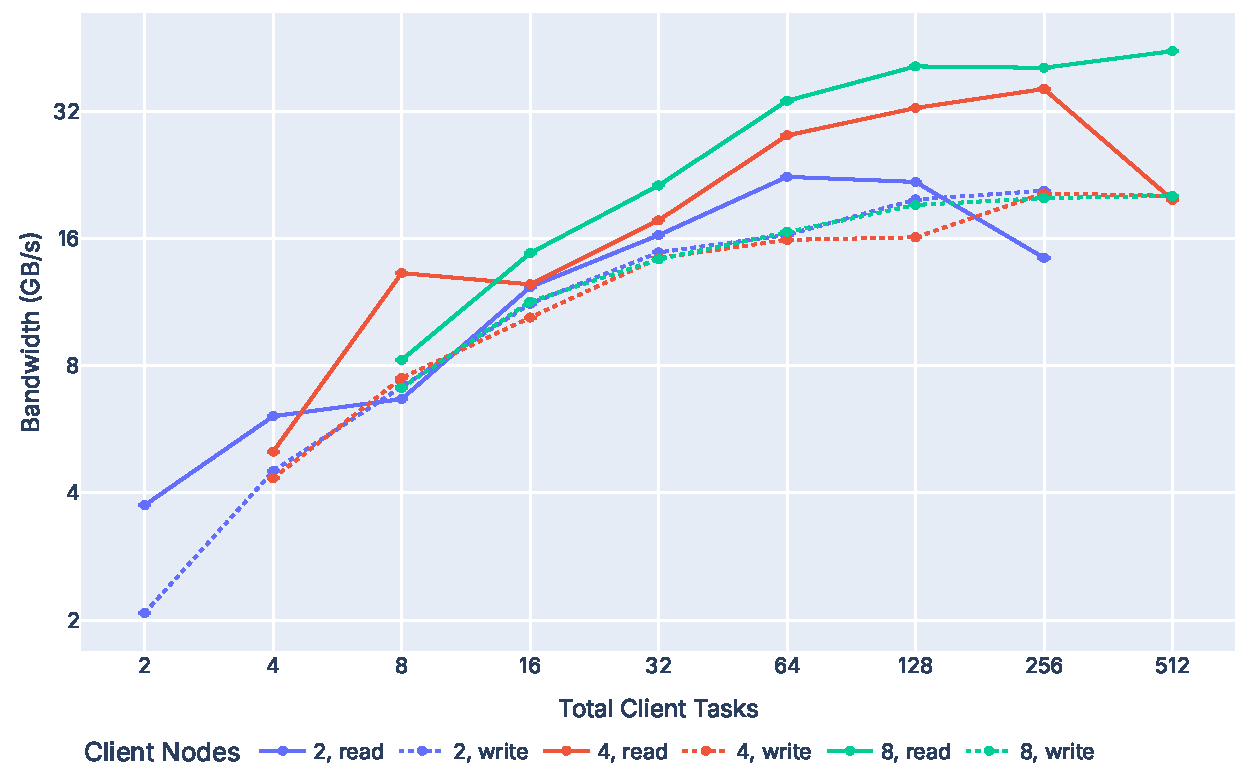
\includegraphics[width=0.9\linewidth]{assets/perf_results/cephfs_ec_seq_64m.pdf}
    \caption[\acs{CephFS} Erasure-Coding 64MiB Sequential Read/Write I/O Performance]{Sequential read/write \acs{I/O} performance of the \acs{CephFS} backend on a mixed 4+2 EC data and replica-3 metadata pool.}
    \label{fig:cephfs-ec-seq-64m}
\end{figure}

\Cref{fig:cephfs-ec-seq-64m} shows similar scaling to that of the replicated configuration. The dropoff in performance for the 2-node/256-task and 4-node/512-task remains, but to a lesser extent than the replicated configuration. Overall performance is more complex: \Cref{fig:cephfs-tcp-ec-ratio-seq-64m} demonstrates that, unlike \ac{RADOS}, the overhead of \ac{EC} is less significant: read performance was somewhat slower than the replicated performance, while write performance with \ac{EC} was generally identical to, or better than, replication. We also observed consistently that in the suspected \acs{CPU}-bottlenecked scenario with 2-node/256-task and 4-node/512-task runs, performance was significantly higher than that of the replicated runs.

\begin{figure}[H]
    \centering
    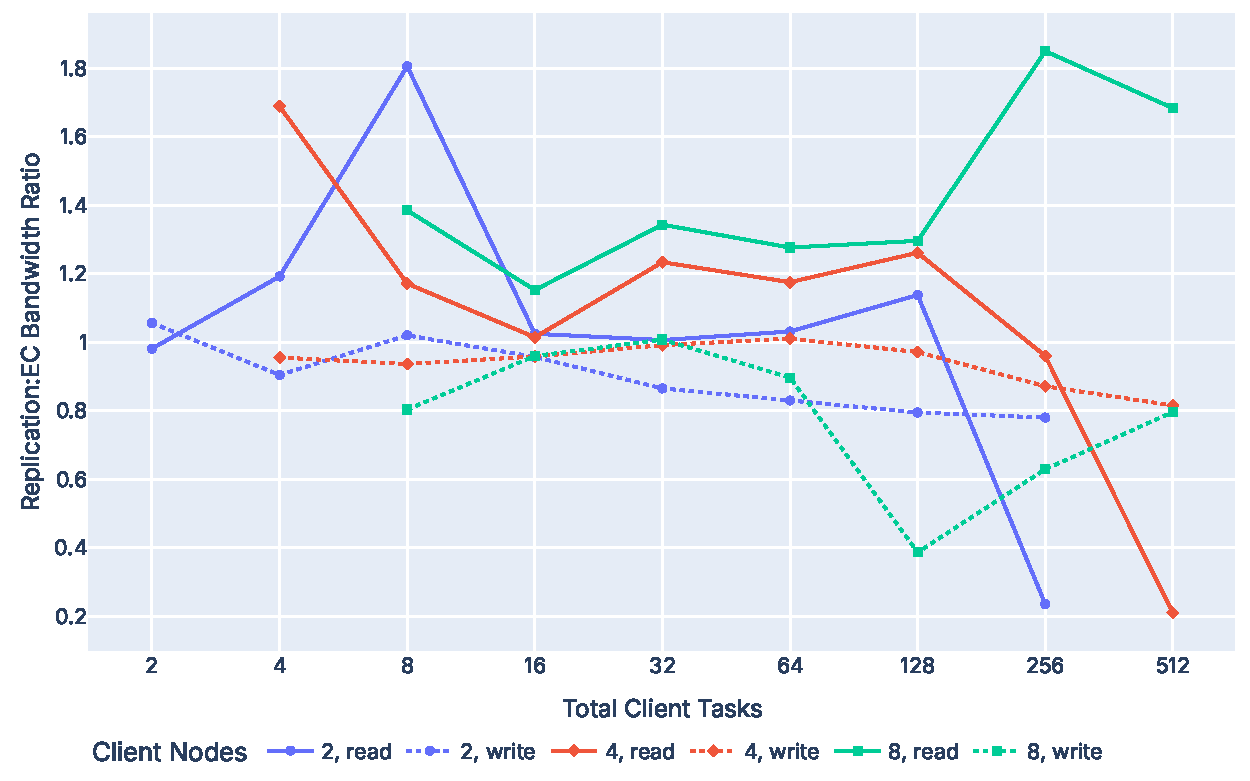
\includegraphics[width=0.9\linewidth]{assets/perf_results/cephfs_tcp_repl_ec_ratio_seq_64m.pdf}
    \caption[\acs{CephFS} Erasure-Coding 64MiB Sequential Read/Write Performance Ratio]{Relative performance ratio of replication over \acs{EC} for the \acs{CephFS} backend.}
    \label{fig:cephfs-tcp-ec-ratio-seq-64m}
\end{figure}

\subsection{Small \acs{I/O} Operations}

For small \ac{I/O} tests on the \ac{RADOS} layer, 2MiB objects were created and written to in 4 KiB increments. For the \ac{CephFS} layer, we additionally performed tests with and without fsync enabled. The behaviour of the \ac{RADOS} backend within \ac{IOR} is not affected by fsync options, as \ac{IOR} uses the synchronous operations provided by the \ac{RADOS} \ac{API}.

\subsubsection{Replicated Performance}

\begin{figure}[htbp]
    \centering
    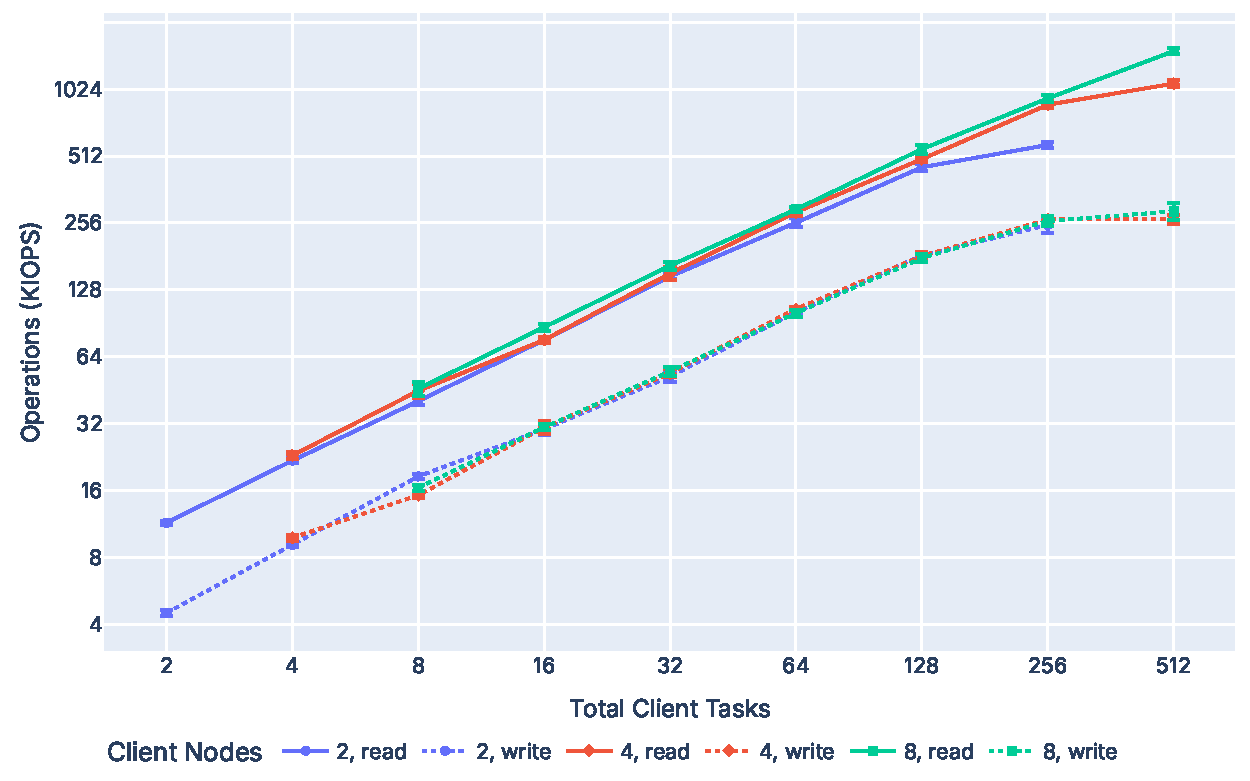
\includegraphics[width=0.9\linewidth]{assets/perf_results/rados_tcp_seq_4k_2m_repl3.pdf}
    \caption[RADOS 4KiB Sequential Read/Write I/O Performance]{Sequential 4KiB read/write I/O performance using the \acs{RADOS} interface.}
    \label{fig:rados-tcp-seq-4k-2m-repl3}
\end{figure}

\Cref{fig:rados-tcp-seq-4k-2m-repl3} shows per-client performance limitations with the \ac{RADOS} backend; read performance is limited to $\leq$ 6K \ac{IOPS} per task, while write performance is limited to $\leq$ 2.5K \ac{IOPS} per task. Unlike the large sequential write results, the performance drop-off at high task counts is much smaller; per-node limitations are also less apparent for small \ac{I/O} operations, likely due to the impacts of network latency. Variance in \ac{IOPS} between runs is low.

\begin{figure}[htbp]
    \centering
    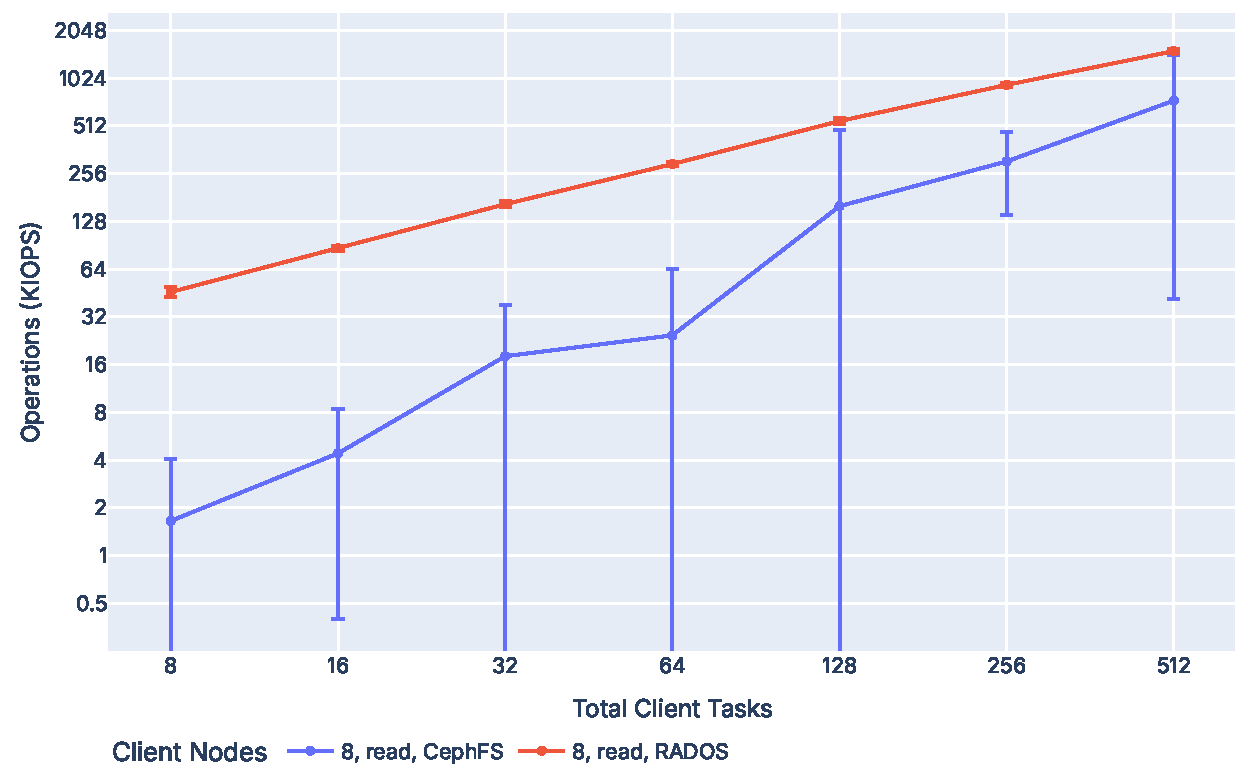
\includegraphics[width=0.9\linewidth]{assets/perf_results/cephfs_tcp_seq_4k_2m_8N.pdf}
    \caption[\acs{CephFS} 4KiB Sequential Read I/O Performance]{Sequential 4KiB read I/O performance for 8 nodes using the \acs{CephFS} interface compared to the \acs{RADOS} interface showing high performance variance.}
    \label{fig:cephfs-tcp-seq-4k-2m-repl3-8N}
\end{figure}

Unlike \ac{RADOS}, \ac{CephFS} demonstrates much higher performance variation. In~\cref{fig:cephfs-tcp-seq-4k-2m-repl3-8N}, we have selected only the 8-node results for readability purposes; however, for all tests, performance is both significantly lower than that of \ac{RADOS}, and variance is significantly higher. This is especially apparent at low client node counts: at 8 nodes and 1 task/node, 4KB sequential reads are 27$\times$ higher on the \ac{RADOS} backend (45.9K \acs{IOPS}) compared to \ac{CephFS} (1.65K \acs{IOPS}). 

\begin{figure}[htbp]
    \centering
    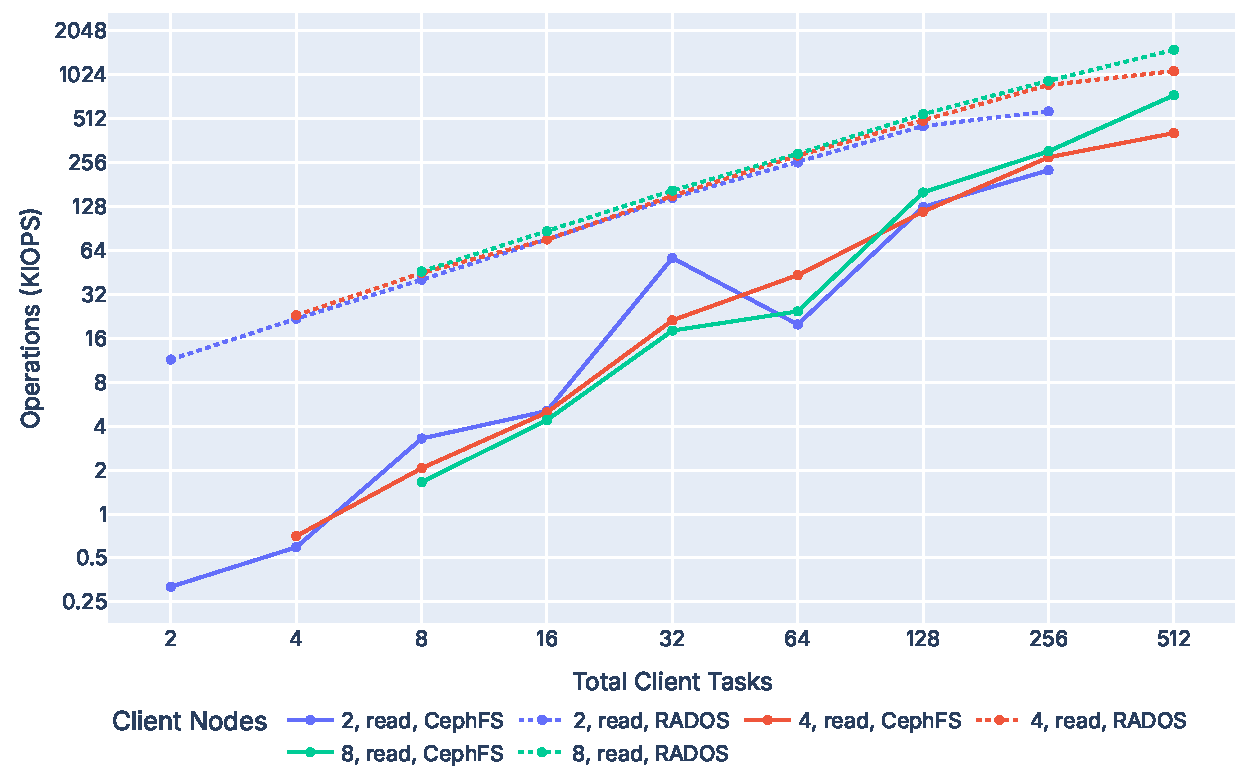
\includegraphics[width=0.9\linewidth]{assets/perf_results/cephfs_tcp_seq_4k_2m_8N_rd_comparison.pdf}
    \caption[\acs{CephFS}/\acs{RADOS} 4KiB Sequential Read I/O Comparison]{Comparison of 4KiB sequential read performance between the \acs{RADOS} and \acs{CephFS} backends, showing similar scaling despite significantly lower performance with \acs{CephFS}.}
    \label{fig:cephfs-tcp-seq-4k-2m-repl3-8N-rd}
\end{figure}

However, although the variance is higher with lower performance, the scaling behaviour is similar to that of the \ac{RADOS} backend as the node count is increased, as shown in~\cref{fig:cephfs-tcp-seq-4k-2m-repl3-8N-rd}.

\begin{figure}[htbp]
    \centering
    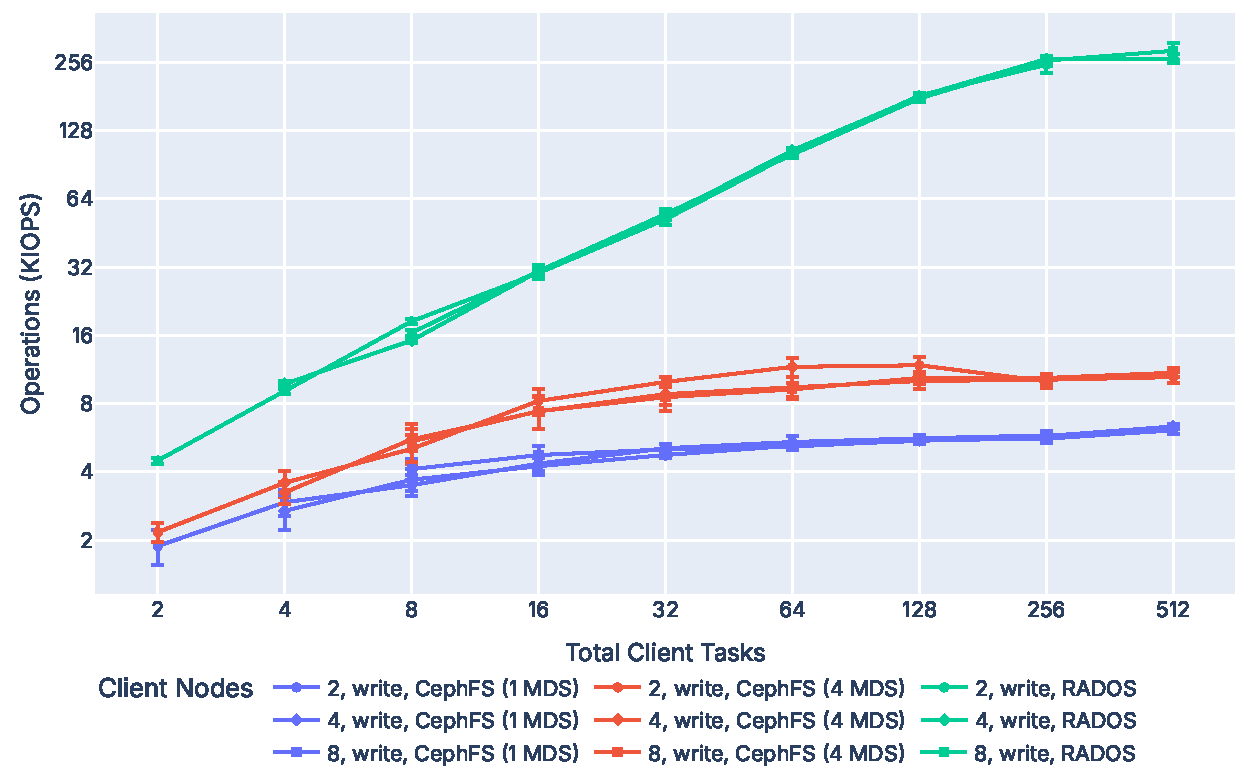
\includegraphics[width=0.9\linewidth]{assets/perf_results/cephfs_tcp_seq_4k_2m_write.pdf}
    \caption[\acs{CephFS}/\acs{RADOS} 4KiB Sequential Write I/O Comparison]{Comparison of 4KiB sequential write performance between the \acs{RADOS} and \acs{CephFS} backends.}
    \label{fig:cephfs-tcp-seq-4k-2m-repl3-8N-wr}
\end{figure}

Write performance on \ac{CephFS}, as shown in~\cref{fig:cephfs-tcp-seq-4k-2m-repl3-8N-wr} is more consistent compared to read performance. However, the \ac{IOPS} seem to be limited by the performance of the \ac{MDS}: a single \ac{MDS} produced approximately 6 k\acs{IOPS} of write performance, while 4 \ac{MDS} daemons with distributed ephemeral pinning enabled produced up to 11 k\acs{IOPS}. The increased number of \ac{MDS} daemons only increased performance if both distributed ephemeral pinning was enabled on the benchmarking folder and when each task created a unique directory; otherwise, performance results for the single \ac{MDS} and 4-\ac{MDS} configuration were identical. The overhead compared to \ac{RADOS} is additionally lower for writes.

\subsubsection{\acs{CephFS} -- Erasure Coding}

\begin{figure}[htbp]
    \centering
    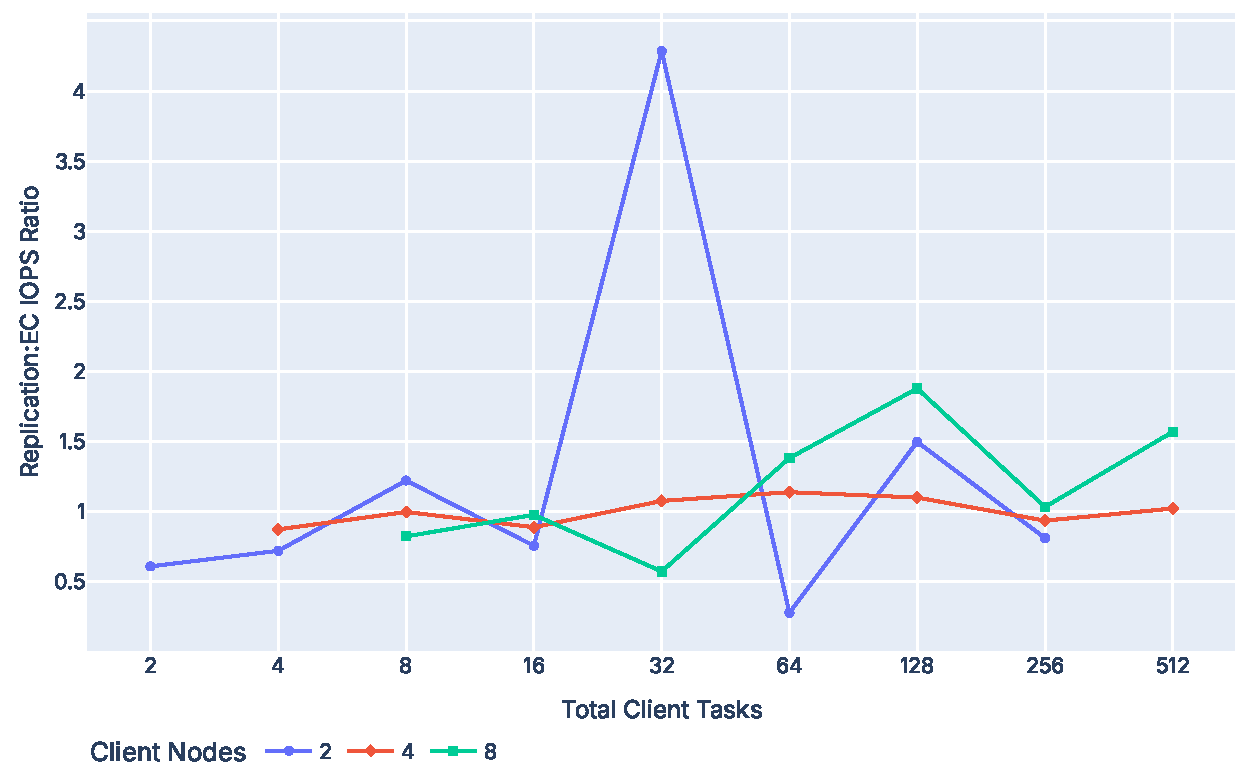
\includegraphics[width=0.9\linewidth]{assets/perf_results/cephfs_repl_ec_ratio_4k_read.pdf}
    \caption[\acs{CephFS} 4KiB Sequential Read I/O Comparison]{Relative read performance of erasure coding over replicated pools with the \acs{CephFS} backend. A higher ratio represents higher replicated performance relative to erasure coding.}
    \label{fig:cephfs-repl-ec-ratio-4k-read}
\end{figure}

\begin{figure}[htbp]
    \centering
    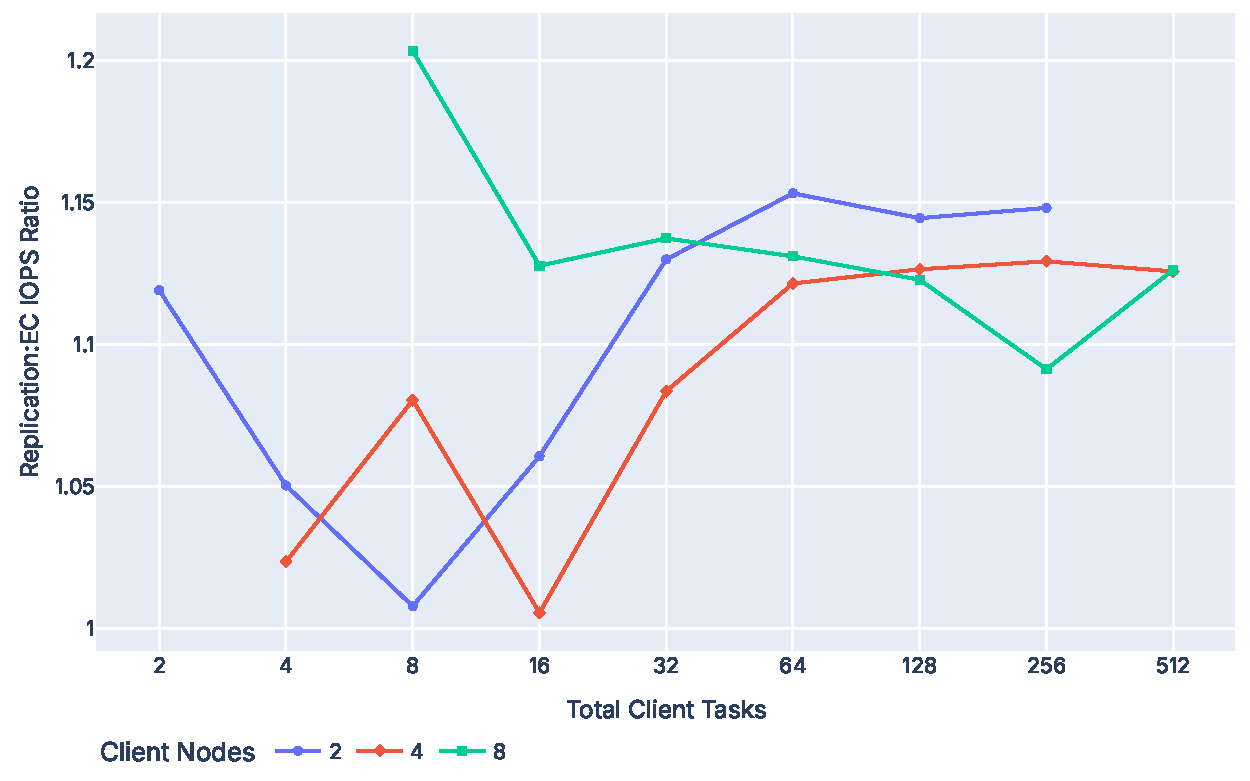
\includegraphics[width=0.9\linewidth]{assets/perf_results/cephfs_repl_ec_ratio_4k_write.pdf}
    \caption[\acs{CephFS} 4KiB Sequential Write I/O Comparison]{Relative write performance of erasure coding over replicated pools with the \acs{CephFS} backend. A higher ratio represents higher replicated performance relative to erasure coding.}
    \label{fig:cephfs-repl-ec-ratio-4k-write}
\end{figure}

\Cref{fig:cephfs-repl-ec-ratio-4k-read}~and~\cref{fig:cephfs-repl-ec-ratio-4k-write} demonstrate the read and write performance ratio of replicated pools over erasure coded \acs{CephFS} pools. Except for an outlier at 2 nodes/32 tasks and 2 nodes/64 tasks, small erasure-coded writes of relatively large objects (2MiB) are not consistently faster or slower than that of replicated writes. Write performance with \ac{CephFS} shows a minor performance penalty for erasure-coding up to approximately 20\% relative to replication, which was observed at 8 nodes/8 tasks.


\pagebreak
\subsection{Metadata Performance}

As the \ac{RADOS} backend does not support the traditional file system layout required for mdtest, we have only performed metadata performance benchmarks using the \ac{CephFS} interface. The options shown in~\cref{tbl:mdtest-configured-options} were provided to mdtest for the performed benchmarks. Additionally, we provided the saveRankPerformanceDetails option to save the results to a file, which we parsed into our storage format as detailed in~\cref{sec:data-collection}.

\begin{table}[htbp]
\centering
\begin{tabular}{|lll|}
\hline
Flag               & Value & Description \\
\hline
\texttt{-n} & 16 & Number of files per task \\
\texttt{-U} & Enabled & Enable rename directory phase \\
\texttt{-R} & Enabled & Random file access \\
\texttt{-L} & Enabled & Files only at leaf level \\
\texttt{-C} & Enabled & Create files \\
\texttt{-T} & Enabled & Stat files \\
\texttt{-E} & Enabled & Read files \\
\texttt{-r} & Enabled & Remove files \\
\texttt{-u} & Enabled & Unique working directory per task \\
\texttt{-i} & 5 & Iteration count \\
\texttt{-w} & 4096 & Bytes to write to file after creation \\
\texttt{-e} & 4096 & Bytes to read from file after write \\
\texttt{-y} & Enabled & Sync file after writing \\
\texttt{-N} & 1 & Enable stride (reordering) for file operations \\
\texttt{-t} & Enabled & Time unique working directory overhead \\
\texttt{-{}-random-seed} & 215098235 & Random \ac{I/O} access seed \\
\hline
\end{tabular}
\caption[Configured mdtest Options]{Flags passed to mdtest for the performed benchmarks.}
\label{tbl:mdtest-configured-options}
\end{table}

\subsubsection{\acs{MDS} Scaling Performance}

To evaluate \ac{MDS} scaling performance, we attempted to eliminate other sources of overhead by limiting the replication factor to replica 1 (i.e., no redundancy). The number of active \ac{MDS} daemons was set to 1, 2, 3, and 4 and scaling results were observed.

It should be noted that several confounding variables in our test environment were not directly controlled. The number of files per \ac{MDS} daemon was determined randomly by the distribution algorithm, and benchmark runs were too short lived and synthetic in nature to allow for us to perform any testing of Ceph's periodic balancing algorithm. These factors may have contributed significantly to the performance variance we observed in our runs.

\lstinputlisting[
    caption={
        [Unutilized \acs{CephFS} \acs{MDS} Daemons]
        Output of \texttt{ceph fs status}, showing the unutilized secondary \ac{MDS} daemons.
    },
    label={lst:mds-no-dist},
    frame=single,
    breaklines=true,
    float
]{assets/ceph/mds_no_dist.txt}

\lstinputlisting[
    caption={
        [\acs{CephFS} \acs{MDS} Load Distribution with Random Pinning]
        Output of \texttt{ceph fs status} after random pinning was enabled, showing inconsistent distribution of tasks.
    },
    label={lst:mds-with-dist},
    frame=single,
    breaklines=true,
    float
]{assets/ceph/mds_with_dist.txt}

Ceph provides two methods for distributing folders in \ac{CephFS} across multiple \ac{MDS} daemons\footnote{\url{https://docs.ceph.com/en/latest/cephfs/multimds/}. Accessed 24.02.2026.}: distributed ephemeral pinning, which pins immediate child folders of selected folders dynamically to the active \ac{MDS} daemons, and random pinning, which allows for recursive pinning of multi-level directory structures randomly across active \ac{MDS} daemons. Without these options configured, operations are directed to a single \ac{MDS}, as shown in~\cref{lst:mds-no-dist}.

Due to the way in which mdtest writes its results and creates files---one output folder, followed by the test directory, followed by per-client folders if enabled---distributed ephemeral pinning did not affect performance. Random pinning required adjustment to settings in order to allow for all directories to be pinned to \ac{MDS} daemons; however, files and folders were distributed successfully across multiple \ac{MDS} daemons with this option. Despite this, we observed that tasks were not always evenly distributed across \ac{MDS} daemons, as shown in~\cref{lst:mds-with-dist}. This inconsistency extended into performance results, as we did not always observe the expected scaling, and observed a very high variance in performance.

\begin{figure}[htbp]
    \centering
    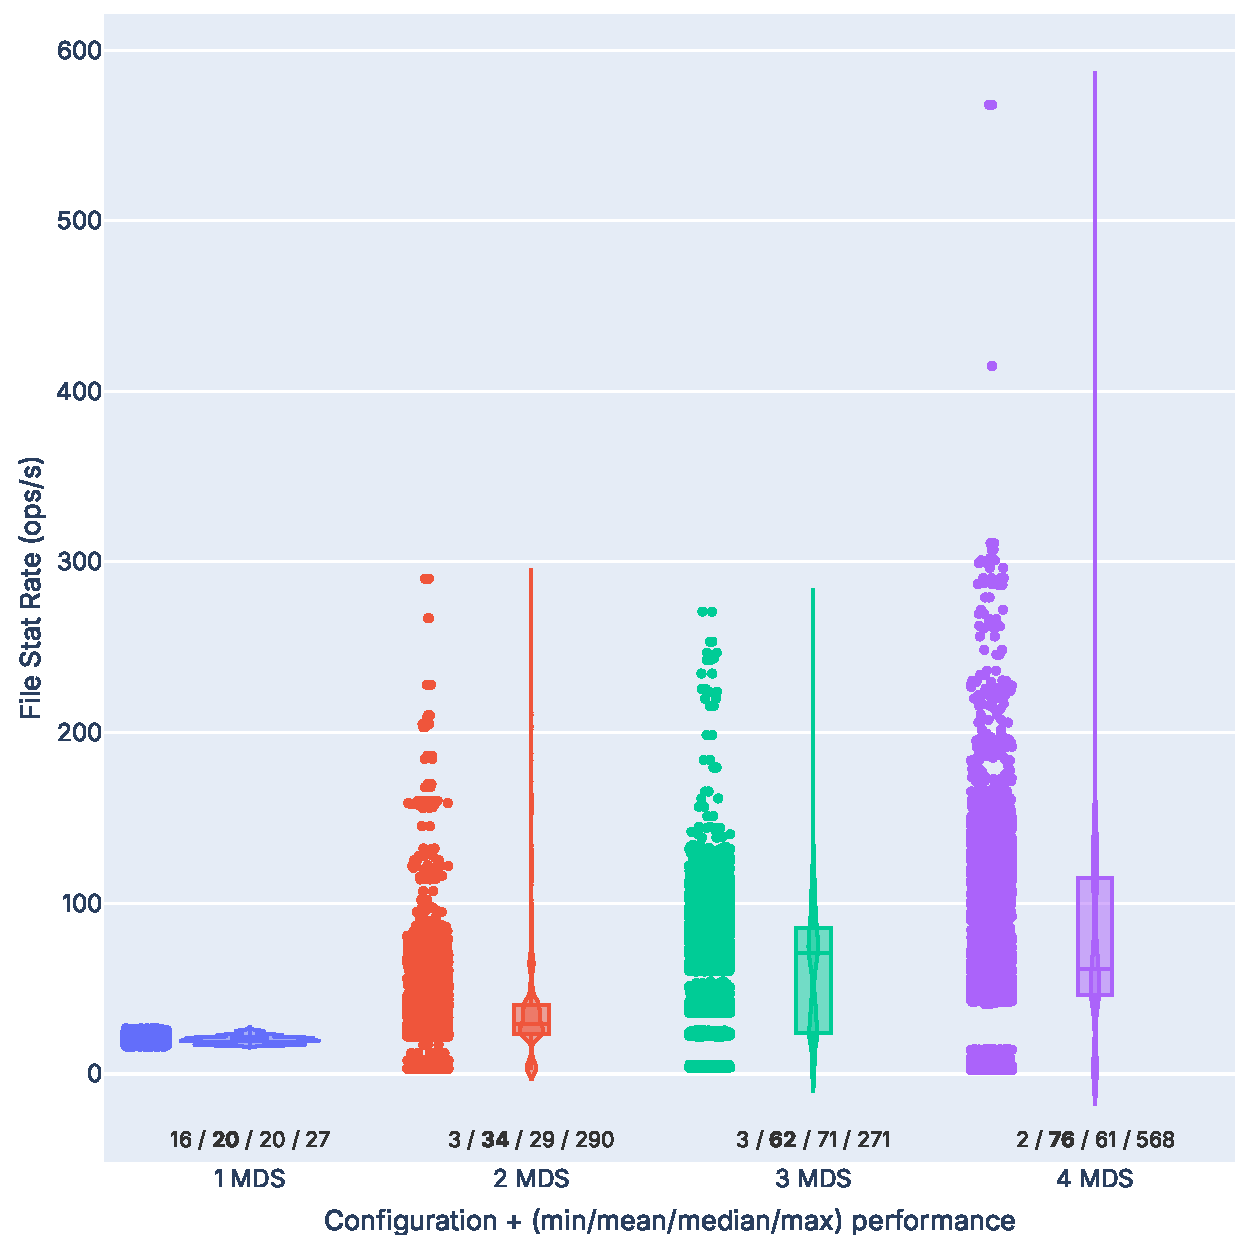
\includegraphics[width=\linewidth]{assets/perf_results/mdtest_violin_file_stat_8nodes_64tpn_mds_scaling.pdf}
    \caption[\acs{CephFS} MDS Scaling Performance -- File Stat Rate (8 nodes)]{Performance of the file stat operation per task with various numbers of active \acs{MDS} daemons with 512 total clients across 8 nodes, showing good scaling, albeit high performance variation.}
    \label{fig:mdtest-violin-file-stat-8n}
\end{figure}

\Cref{fig:mdtest-violin-file-stat-8n} shows the file stat rate observed at a per-task level. This specific run shows good performance scaling results; however, the large performance variance is likely due to the inconsistent distribution of client folders to \ac{MDS} daemons---clients which are on more lightly-loaded \ac{MDS} daemons are likely to have more performance available to them. Certain tasks in the 2- and 3-\acs{MDS} configurations seem to be severely performance-starved, which may be indicative of an overloaded \ac{MDS} daemon due to the inconsistent distribution.

\begin{figure}[H]
    \centering
    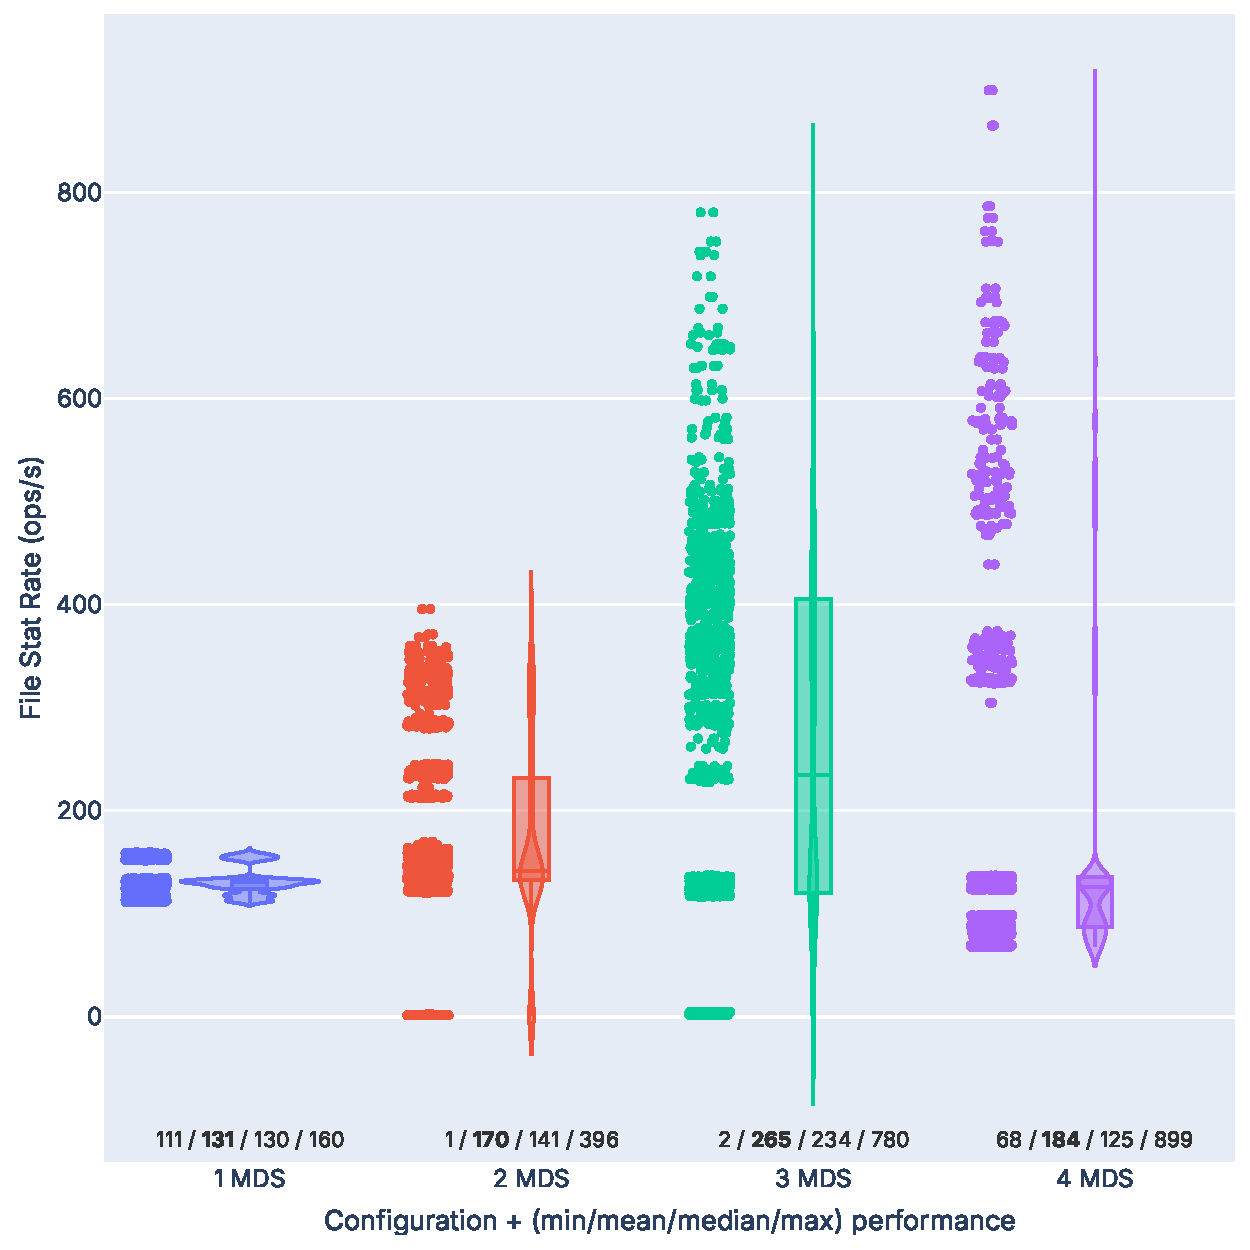
\includegraphics[width=1\linewidth]{assets/perf_results/mdtest_violin_file_stat_2nodes_64tpn_mds_scaling.pdf}
    \caption[\acs{CephFS} MDS Scaling Performance -- File Stat Rate (2 nodes)]{Performance of the file stat operation per task with various numbers of active \acs{MDS} daemons with 256 total clients across 2 nodes, showing inconsistent scaling results.}
    \label{fig:mdtest-violin-file-stat-2n}
\end{figure}

\Cref{fig:mdtest-violin-file-stat-2n} shows the file stat rate observed at a per-task level. In contrast to the 8-node results, these 2-node results show inconsistent performance scaling, with the 4-node configuration dropping below the performance of the 3-node configuration. The performance starvation of certain tasks is also observed in this run.

\subsubsection{Erasure-Coded Pools}

\begin{figure}[H]
    \centering
    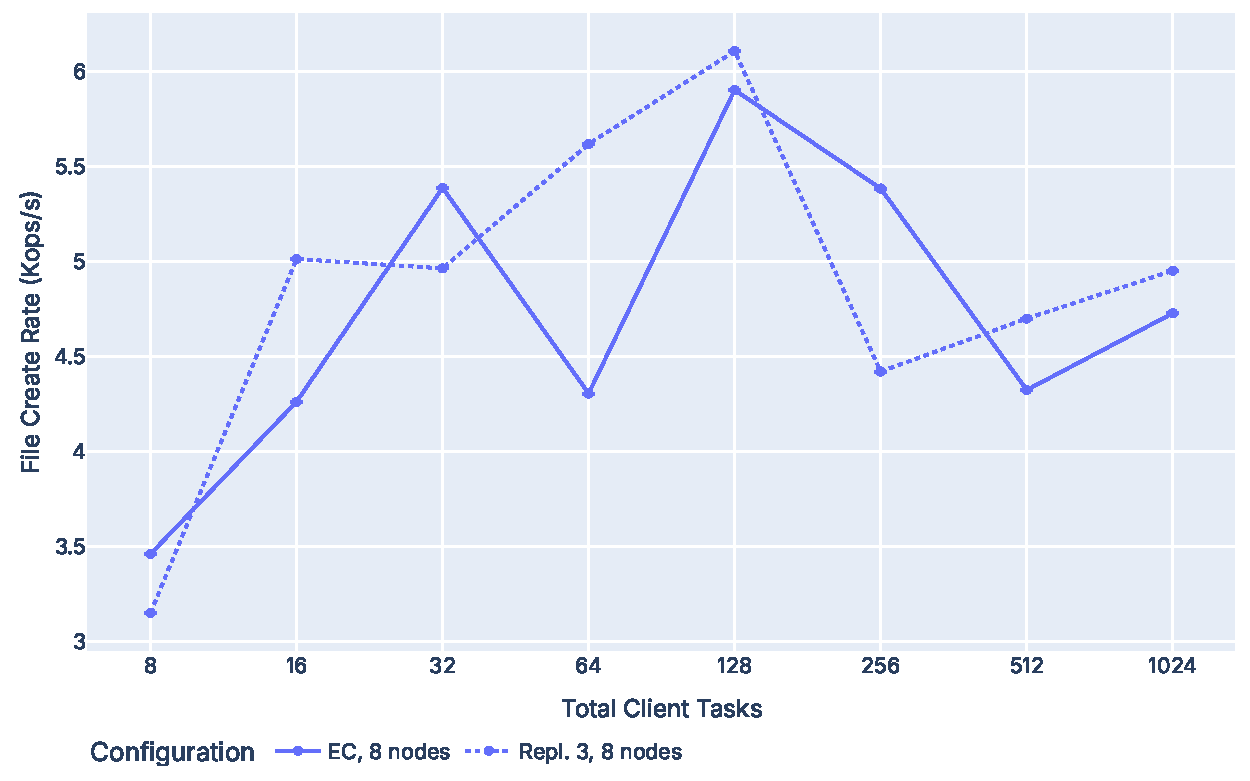
\includegraphics[width=0.9\linewidth]{assets/perf_results/mdtest_file_create_ec_vs_replicated.pdf}
    \caption[\acs{CephFS} Erasure-Coded File Creation Performance]{Performance of file creation operations on erasure-coded pools compared to replicated pools, showing similar performance ranges.}
    \label{fig:mdtest-file-create-ec-replicated}
\end{figure}

Erasure-coded pools demonstrated near-identical performance for metadata operations, such as file/folder creation and deletion. \Cref{fig:mdtest-file-create-ec-replicated} shows the file creation performance of an erasure-coded pool over a replicated pool for an 8-client-node benchmark run, showing similar performance. This is likely due to the fact that the \ac{MDS} metadata pool, which services such operations, uses the same replica-3 profile for both pool types---Ceph does not allow for the use of erasure-coded metadata pools. Therefore, identical performance is to be expected, and the gathered performance results support this.

% This section was commented out due to the fact that the amount of changes that we made to the IO500 benchmark rules would have made the results incomparable to the official IO500 results. 
% This is explained in the discussion section.

\pagebreak
\subsection{System Administration}
\label{sec:system-admin}

The previous sections of our evaluation primarily focused on performance using our custom deployment scripts. However, in order to complete our evaluation of the Ceph file system, we have additionally evaluated Ceph's official deployment tools on our test cluster. To that end, we will detail our findings in this section.

Ceph's setup differs significantly to that of a traditional \ac{HPC} file system. Specifically, the containerization of Ceph services results in particularly relaxed requirements for the host operating system. In addition to the most common \ac{HPC} operating systems on the TOP500 list\footnote{\url{https://top500.org/statistics/sublist/}. Accessed 26.02.2026.}, such as Red-Hat derivatives (e.g., Rocky Linux) and Ubuntu, system requirements are relaxed such that any modern Linux distribution with the base requirements is adequate for a functional Ceph installation\footnote{\url{https://docs.ceph.com/en/reef/cephadm/install/\#requirements}. Accessed 26.02.2026.}---the internal container image is based on CentOS Stream 9\footnote{Checked using the \texttt{/etc/os-release} file within the Ceph containers deployed with cephadm.}.

\subsubsection{Initial Setup}

The following steps were taken in order to build a functional cluster on our virtual machine setup based on the Ceph instructions\footnote{\url{https://docs.ceph.com/en/reef/cephadm/install/}. Accessed 26.02.2026.}:

\begin{sloppypar}
\begin{itemize}
    \item Cephadm was installed using the curl-based method
    \item \texttt{cephadm bootstrap} was used to bootstrap the cluster on the first node \texttt{cvm1}
    \item The created \ac{SSH} public key was copied to the root user's authorized keys of the other nodes in the cluster
    \item \texttt{ceph orch host add cvmX --labels \_admin} was used from \texttt{cvm1} (with X being 2--8), in order to add \texttt{cvm2}--\texttt{cvm8} to the cluster
    \item \acp{OSD} were added based on available hard disks using the command \texttt{ceph orch apply osd -{}-all-available-devices}
\end{itemize}
\end{sloppypar}

\subsubsection{Accessing the Ceph Dashboard}

After initial bootstrapping, we were presented with credentials, which we were able to use to access the Ceph dashboard.

\lstinputlisting[
    caption={
        [Ceph Bootstrap Output]
        Output at the end of the Ceph bootstrapping phase, showing the credentials for accessing the Ceph dashboard.
    },
    label={lst:ceph-bootstrap},
    frame=single,
    breaklines=true
]{assets/ceph/bootstrap_output.txt}

\pagebreak
\begin{figure}[H]
    \centering
    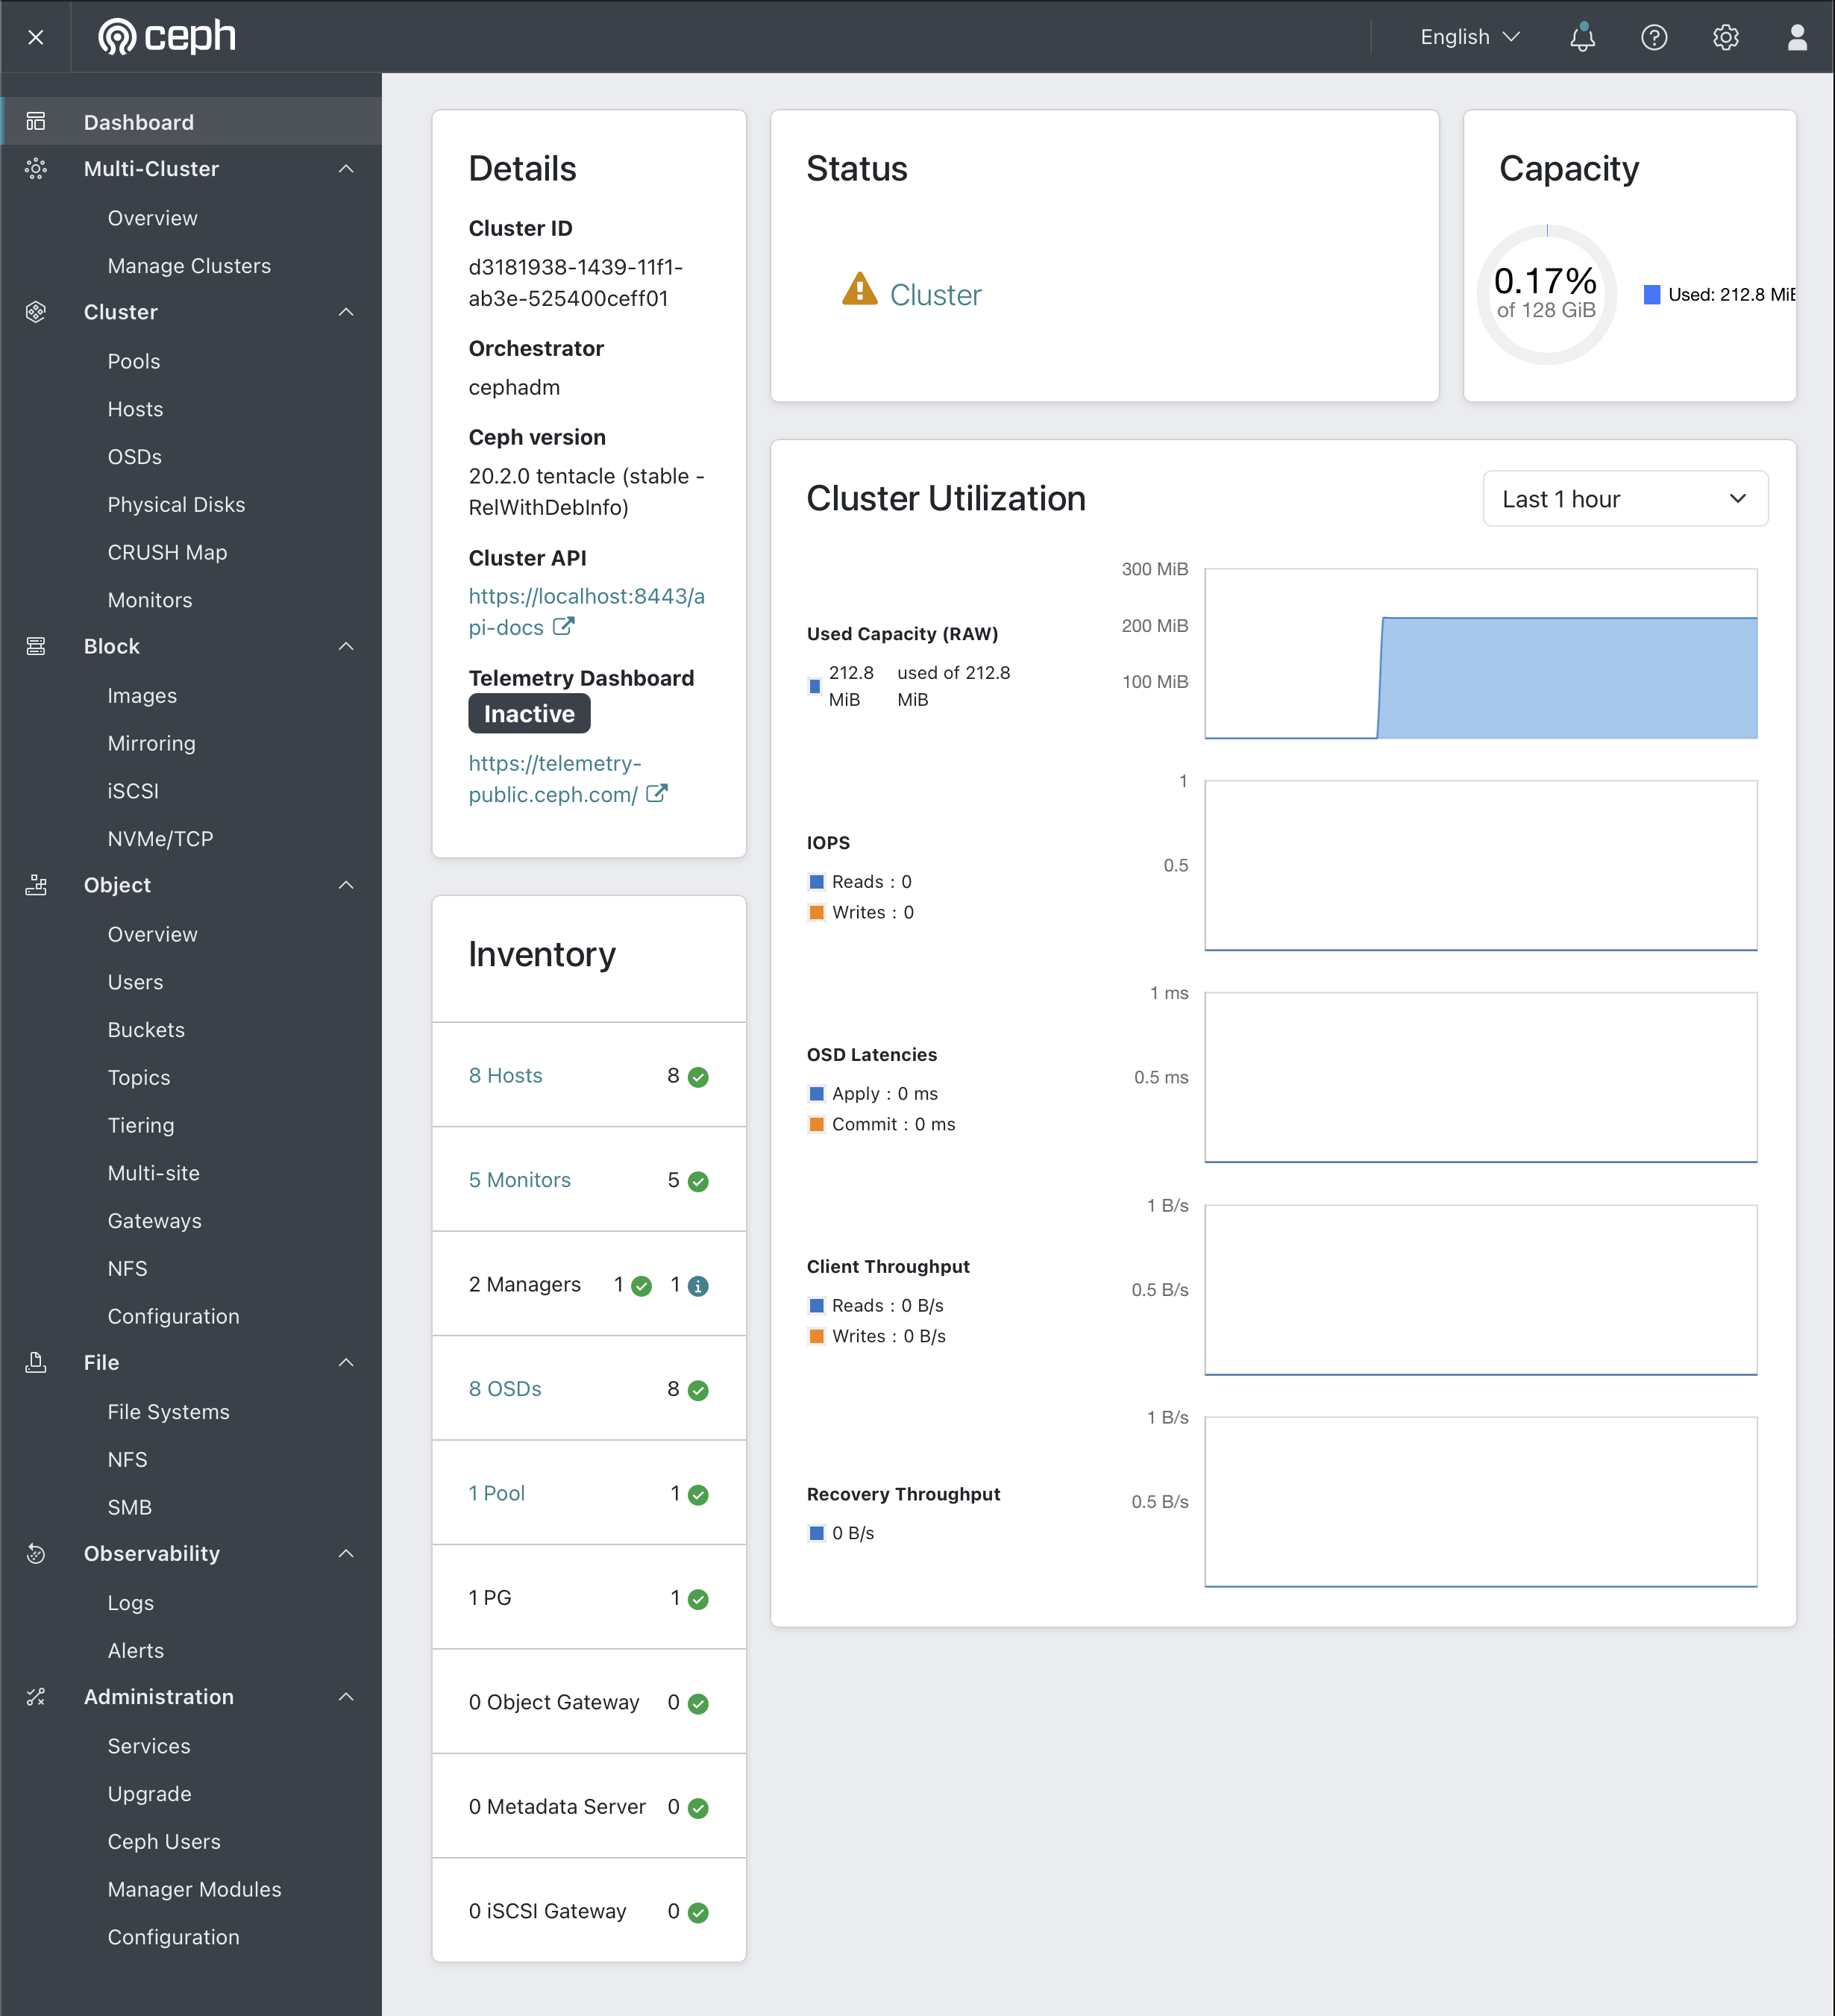
\includegraphics[width=0.99\textwidth]{assets/ceph/ceph-dashboard.png}
    \caption{The Ceph Dashboard}
    \label{fig:ceph-dashboard}
\end{figure}

The Ceph dashboard provides a web-based interface for monitoring and managing the cluster without the need for experience with the Ceph \ac{CLI}. A screenshot of the dashboard of the deployed cluster is shown in~\cref{fig:ceph-dashboard}. We were able to perform common monitoring tasks successfully using the dashboard, such as viewing free space, monitoring disk activity, and checking other health metrics of the cluster. In addition to these basic features, the dashboard is also capable of performing more advanced tasks\footnote{\url{https://docs.ceph.com/en/quincy/mgr/dashboard}. Accessed 26.02.2026.}, and is being actively developed. The monitoring stack is based on Prometheus, which allows for a high degree of customizability and external access, in addition to integration with other tools such as Grafana.

\pagebreak
\subsubsection{Potential System Administration Issues}
\label{sec:system-admin-issues}

We have identified a number of minor issues and bugs in Ceph's system administration aspect.

\subsubsection*{User Interface Inconsistency}

Adding \acp{OSD} via \texttt{ceph orch} worked as expected. However, the user interface refresh delay resulted in some confusion, as the status of the disks was not immediately updated. We added the disks to the cluster with the orchestrator as shown in~\cref{lst:osd-add-initial}.

\lstinputlisting[
    caption={Adding \acsp{OSD} via \texttt{ceph orch}},
    label={lst:osd-add-initial},
    frame=single,
    breaklines=true
]{assets/ceph/osd_add_initial.txt}

However, the outputs from various Ceph daemons took several minutes to synchronize with each other, which caused some confusion when determining the cluster's actual state. \Cref{lst:osd-sync-issue} demonstrates the inconsistent reporting of various Ceph commands.

\lstinputlisting[
    caption={
        [\acs{OSD} Synchronization Delay]
        \acs{OSD} synchronization delay after adding disks. The device list shows available disks, but the \acsp{OSD} are reported as down. Outputs are truncated.
    },
    label={lst:osd-sync-issue},
    frame=single,
    breaklines=true
]{assets/ceph/osd_sync_issue.txt}

\begin{sloppypar}
In order to synchronize the system, restarting the manager daemons was required, for which we used \texttt{ceph orch restart mgr}. After this step, the status commands showed the expected output, as shown in~\cref{lst:osd-after-restart}.
\end{sloppypar}

\lstinputlisting[
    caption={
        [\acs{OSD} Status After Manager Daemon Restart]
        \acs{OSD} status after a restart of the manager daemons.
    },
    label={lst:osd-after-restart},
    frame=single,
    breaklines=true
]{assets/ceph/osd_after_restart.txt}

\subsubsection*{Adding \ac{OSD} Disks}

When attempting to check the system for new \acp{OSD}, the reject reason does not clearly state that the reason specific \acp{OSD} may be rejected are due to the fact that these disks already host a Ceph \ac{OSD}, as the error message states only that a file system is on the disk, not necessarily one used by Ceph, as shown in~\cref{lst:osd-reject-reasons}.

\lstinputlisting[
    caption={
        [\acs{OSD} Rejection Reasons for Existing Ceph Disks]
        Rejection reasons for existing Ceph disks when attempting to add \acsp{OSD}.
    },
    label={lst:osd-reject-reasons},
    frame=single,
    breaklines=true
]{assets/ceph/osd_reject_reasons.txt}

\subsubsection*{Reinstallation Quirks}

In the Ceph documentation, it is mentioned that a cluster can be purged with cephadm\footnote{\url{https://docs.ceph.com/en/quincy/cephadm/operations/}. Accessed 26.02.2026.}. However, we found that this did not cleanly purge all traces of the cluster, leaving behind residual daemons which complicated future reinstallations of the cluster due to clashes with existing daemons left behind on the cluster, including after a reboot.

\lstinputlisting[
    caption={
        [Residual Node-Exporter Daemons]
        Residual node-exporter container remaining after the cluster purge command was run.
    },
    label={lst:residual-node-exporter},
    frame=single,
    breaklines=true
]{assets/ceph/residual_node_exporter.txt}

\lstinputlisting[
    caption={
        [Residual Ceph Daemons]
        Residual Ceph daemons from multiple clusters remaining after the cluster purge command was run.
    },
    label={lst:residual-daemons},
    frame=single,
    breaklines=true
]{assets/ceph/residual_daemons.txt}

When we manually removed the containers after running the Ceph purge and restarted the virtual machines, we were able to successfully initialize a new cluster from scratch.

% Modern Ceph deployments rely on the use of the \texttt{cephadm} tool. Because this tool uses standard \ac{SSH} connections to connect to and set up hosts, as well as Podman as a container runtime for running Ceph daemons

% In this section, we primarily discuss the system administration of the Ceph file system, from cluster setup to common maintenance tasks.

% Setup of the cluster was rather straightforward, and documentation on the bootstrapping phase was clear and concise. The cephadm tool was downloaded on the host node, and bootstrapping was performed successfully

\subsection{Reflection on Goals}
\label{sec:reflection-on-goals}

Returning to our goals discussed in the thesis introduction, we reflect on the extent to which each has been addressed.

\begin{itemize}
    \item Our comparison of \ac{RADOS} and \ac{CephFS} on the same cluster successfully isolated the overhead introduced by the file system layer, revealing minimal overhead for large sequential \ac{I/O}~(\Cref{fig:cephfs-tcp-seq-64m-repl3}) but significant penalties for small \ac{I/O} operations~(\Cref{fig:cephfs-tcp-seq-4k-2m-repl3-8N}). Additionally, \ac{CephFS} write performance was constrained by \ac{MDS} throughput~(\Cref{fig:cephfs-tcp-seq-4k-2m-repl3-8N-wr}).

    \item Our scalability evaluation using \ac{IOR} and mdtest demonstrated strong, close to linear read scaling with the \ac{RADOS} interface~(\Cref{fig:rados-tcp-seq-64m-repl3-pernode-normalized}), but highlighted \ac{MDS} limitations at the \ac{CephFS} layer~(\Cref{fig:mdtest-violin-file-stat-8n,fig:mdtest-violin-file-stat-2n}), at least in the context of our limited test setup, which used random folder pinning in order to produce scaling results with mdtest.

    \item Our evaluation of network fabrics was partially achieved. \ac{TCP} over InfiniBand was able to saturate the network link~(\Cref{sec:results-network-bandwidth-ib}), while Omni-Path \ac{TCP} throughput was significantly constrained by \ac{CPU} processing overhead~(\Cref{sec:results-network-bandwidth-opa}). Our initial benchmarks of Ceph on the Omni-Path fabric showed promising scaling results~(\Cref{fig:omnipath-seq-64m}), but a kernel vulnerability in the \texttt{hfi1} driver~(\Cref{sec:opa-bad-root-cause-analysis}) prevented a complete evaluation.

    \item Our analysis of replication and \acl{EC} performance trade-offs showed the benefits of erasure coding for disk-limited workloads~(\Cref{fig:128pg-write-scaling}). At scale, \ac{EC} write performance was mostly comparable to replication for both \ac{RADOS}~(\Cref{fig:rados-tcp-repl-ec-ratio-seq-64m}) and \ac{CephFS}~(\Cref{fig:cephfs-tcp-ec-ratio-seq-64m}). Metadata operations were unaffected by pool type~(\Cref{fig:mdtest-file-create-ec-replicated}), which was expected, due to the common replica-3 metadata pool configuration.

    \item Finally, in the system administration perspective, our goals were partially met. The Cuttlefish framework we developed demonstrated the feasibility of rootless Ceph deployment on \ac{HPC} nodes for architectural benchmarking purposes, while our evaluation of the cephadm tool was generally positive, despite some minor usability issues~(\Cref{sec:system-admin-issues}). However, we were unable to perform a large-scale test of Ceph with physical storage devices, especially high-performance \acp{SSD}, which would have allowed us to evaluate Ceph's performance under production-grade conditions.      
\end{itemize}

\subsubsection{Deployment Recommendations}
\label{sec:deployment-recommendations}

Based on our findings, we offer the following practical considerations for deploying Ceph in \ac{HPC} environments:

\begin{itemize}
    \item Erasure-coded pools should be considered for archival storage with predominantly large, sequential \ac{I/O} patterns, where they can offer better storage efficiency compared to replication, with better performance for these scenarios when disk performance is write-limited~(\Cref{fig:128pg-write-scaling,fig:rados-tcp-repl-ec-ratio-seq-64m,fig:cephfs-tcp-ec-ratio-seq-64m}). Replicated pools remain preferable for latency-sensitive or metadata-heavy workloads, such as home, scratch, and application data directories.

    \item The per-task \ac{IOPS} ceiling we observed~(\Cref{fig:rados-tcp-seq-4k-2m-repl3}), wihhc has been corroborated at larger scales~\cite{ceph-1tib}, suggests that single-threaded or low-concurrency applications may not benefit from Ceph's aggregate throughput capabilities. Based on our large sequential \ac{I/O} results~(\Cref{fig:rados-tcp-seq-64m-repl3}), we suggest that workloads should be designed to use sufficient levels of parallel \ac{I/O}, ideally across multiple client nodes, in order to make efficient use of Ceph's capabilities.

    \item For workloads generating high metadata loads, such as \ac{AI} training pipelines or code compilation tasks, the loopback mount approach~\cite{Krotkiewski_2017} is worth considering. Our mdtest and small \ac{I/O} results~(\Cref{fig:mdtest-violin-file-stat-8n,fig:mdtest-violin-file-stat-2n,fig:cephfs-tcp-seq-4k-2m-repl3-8N-wr}) show that \ac{MDS} performance remains a bottleneck even with multiple daemons, and shifting the \ac{I/O} load onto the more scalable \ac{RADOS} layer could alleviate this, provided the application can work with an overlay file system. However, we were unable to evaluate the performance of the loopback mount approach in our benchmarks due to limited permissions.

    \item Ceph's \acs{TCP}-based messenger implementation can put significant pressure on the host's network stack. Our network benchmarks~(\Cref{fig:ib-tcp-throughput,fig:opa-tcp-throughput}) and the kernel-level failures encountered on Omni-Path~(\Cref{sec:opa-bad-root-cause-analysis}) demonstrate that deployment on networks with performant stateless \ac{TCP/IP} hardware offload support, such as Ethernet or modern InfiniBand networks, is advisable over fabrics with limited \ac{TCP} offload capabilities, such as Omni-Path.
\end{itemize}

% !TEX root = main.tex
\pagebreak
\section{Discussion}
\label{sec:discussion}

\subsection{Architectural Stability}

Our analysis of the Ceph file system at both the \ac{RADOS} and \ac{CephFS} layers shows that data throughput scales well, particularly when the file system is subjected to high-concurrency workloads with large file accesses. Ceph's decentralized approach using \ac{CRUSH} ensures that an increasing number of clients distribute their workloads across all available \acp{OSD} on the system. However, the per-task performance using \ac{TCP} is low compared to the overall achievable throughput, which could pose a potential challenge for workloads which use a single-rank file access pattern. This per-node performance ceiling is consistent with findings from larger-scale deployments: benchmarks at Clyso~\cite{ceph-1tib} reported a similar per-node \ac{IOPS} limitation of 400--600K random read \ac{IOPS}, which they likely attributed to Ceph's \ac{OSD} threading model and messenger implementation: this persisted regardless of the underlying storage performance. However, provided that the file access patterns are sufficiently parallel, Ceph can be a capable system for \ac{HPC} scratch or archival storage with large block \ac{I/O} patterns.

While the data-path results were encouraging, metadata performance within Ceph lies in stark contrast to \ac{RADOS} with a complex performance profile. Metadata operations, such as file creation and deletion, directory listings, and index node queries, do not demonstrate the same strong scaling performance across runs in the same way that \ac{RADOS} does. Ceph's \ac{MDS} daemons are responsible for all metadata operations at the \ac{CephFS} layer, resulting in a performance bottleneck. While the number of active \ac{MDS} daemons may be increased by changing the max\_mds parameter within the Ceph configuration, the benchmarking data suggest that scaling is not as straightforward as adding \ac{MDS} daemons to the cluster---performance rarely scales linearly with the number of \ac{MDS} daemons, and care must be taken in order to optimize file and folder layouts such that they can be distributed across multiple \ac{MDS} daemons evenly. A large number of methods are available for partitioning of folder structures across \ac{MDS} daemons, including automatic subtree partitioning, but it may be necessary for system administrators to consider whether manual adjustment of the placement policy is necessary. In our testing with random subtree pinning, Ceph did not consistently demonstrate the expected performance uplift with an increased number of \ac{MDS} daemons, as some \ac{MDS} ranks received a significantly higher share of files and folders relative to others, resulting in inefficient utilization.

Further empirical evaluation is required in order to validate whether our observed throughput inconsistencies stem from the inherent limitations of the \ac{MDS}, especially in real-world conditions. Our specific approach of subtree pinning, necessitated by the nature of our synthetic benchmarks, could have resulted in the suboptimal allocation of directories to \ac{MDS} daemons. In addition, we did not test features such as automatic subtree rebalancing based on collected load information due to the short-lived nature of the benchmark runs leaving no time for the subtree balancer to run.

\subsubsection{Write Performance}

A notable finding from our large-scale benchmarks is the write performance limitation observed with replicated pools on the \ac{RADOS} layer. Write throughput reached 10--15\,GiB/s regardless of the number of client nodes, while read throughput continued to scale well with additional nodes. The bottleneck appears to be on the cluster side during writes. In a replica-3 configuration, each client write triggers two additional writes between \acp{OSD}~\cite{ceph-paper}, tripling the internal network traffic relative to reads. This write amplification likely results in saturation of network resources on the cluster side before the client nodes are fully utilized. However, the read-to-write performance ratio in our benchmarks generally exceeded 3:1 at higher node counts, where a 3:1 ratio would be expected from write amplification alone. This suggests additional overhead from write operations within the \acp{OSD}. The Clyso evaluation~\cite{ceph-1tib} observed a related issue at scale, where placement groups entered a ``laggy'' state under high write concurrency, further degrading write throughput---an issue attributed to messenger overhead or contention within the \ac{OSD}.

\subsubsection{Applying In-Memory Results to Production}

Our evaluation employed two complementary benchmarking environments: an in-memory deployment for high-performance testing on the \ac{HPC} cluster, which isolates Ceph's software overhead by eliminating storage media as a bottleneck, and a controlled lab deployment with disk \ac{I/O} throttling at 50\,MiB/s per \ac{OSD}, which allows us to observe Ceph's behaviour under well-defined constraints. By connecting the results from both environments, we can provide a more complete picture of expected real-world performance.

The in-memory benchmarks establish a performance ceiling: for example, sequential write throughput with replica-3 \ac{RADOS} pools plateaued at 10--15\,GiB/s regardless of the number of client nodes, and per-node read throughput saturated slightly above 100\ Gbit/s. These figures represent the maximum throughput achievable when storage media is not a limiting factor, and is instead bounded by Ceph's and the host's networking stack as well as internal \ac{OSD} processing overhead. In a production deployment, actual throughput will be the minimum of this software ceiling and the aggregate throughput of the storage media in use, which is especially relevant for slow storage media such as \acp{HDD}.

Our lab benchmarks provide a complementary data point: with disk performance throttled to a known level, Ceph achieved approximately 70--80\% of the theoretical aggregate disk throughput for replicated pools. Combining this disk efficiency factor with the software ceiling from our in-memory results, the expected throughput of a production deployment can be estimated. If the aggregate disk throughput, taking into consideration the overhead of the pool type (replication or \ac{EC}), falls below the software ceiling, the deployment will likely be disk-limited, and the 70--80\% efficiency we observed in our lab benchmarks provides an estimate of the achievable performance. However, this 70--80\% efficiency factor is derived from slow (50\,MiB/s) virtual disks, and cannot be safely generalized to fast physical media such as modern \ac{NVMe} \acp{SSD}, due to the possibility of \ac{CPU} bottlenecks within the BlueStore backend. If the aggregate disk throughput exceeds the software ceiling, as would be the case with high-performance network adapters and a large number of high-performance \acp{SSD}, the deployment will likely be software-limited: our in-memory results provide the upper bound which can be applied to this scenario. Furthermore, additional overhead introduced by BlueStore is not accounted for in our MemStore benchmarks, and may further reduce throughput in disk-limited scenarios.

\subsection{Network Performance}

Our experimental results highlight the importance of the role of high-performance networking in Ceph's storage performance. Ceph's reliance on the regular \ac{TCP/IP} stack introduces latency and throughput penalties, especially at small file sizes, which reduced overall performance for certain access patterns. Unlike incumbent \ac{HPC} file systems, Ceph does not provide a production-grade \ac{RDMA} transport: while the experimental \ac{RDMA} transport was tested in this thesis, we observed poor scaling results as well as the failure to achieve higher peak throughput relative to \acs{TCP} for large file accesses. However, small-file accesses as well as accesses with low numbers of clients proved significantly faster with \ac{RDMA}, likely due to its lower \ac{CPU} overhead and end-to-end latency characteristics.

Even though the \ac{RDMA} transport is available and may perform better in certain narrow edge cases, the experimental and undocumented nature of this feature is unlikely to be of use in current \ac{HPC} clusters due to its instability and uncertain future prospects with the introduction of the Crimson backend.

\subsection{\acs{CephFS} Overhead}

A direct comparison of the \ac{RADOS} and \ac{CephFS} results we gathered on the same cluster allows for us to quantify the overhead introduced by the \ac{CephFS} layer. For large sequential \ac{I/O} (64\,MiB), the \ac{CephFS} throughput scaled similarly to \ac{RADOS}, indicating that the \ac{CephFS} overhead is minimal for bulk data transfers where the \ac{MDS} is only involved at the beginning and end of the transfer for the file open/close operations. However, for small \ac{I/O} operations (4\,KiB), the overhead was substantial: at 8 nodes with 1 task per node, \ac{RADOS} achieved 45.9K read \ac{IOPS} compared to 1.65K for \ac{CephFS}---a 27$\times$ difference. This gap narrowed at higher concurrency levels, but \ac{CephFS} consistently remained an order of magnitude slower than \ac{RADOS} for small reads. Write performance showed a smaller overhead, with the \ac{MDS} becoming the primary bottleneck: a single \ac{MDS} produced approximately 6\ k\acs{IOPS}, while 4 \ac{MDS} daemons with distributed pinning achieved up to 11\ k\acs{IOPS}. These findings suggest that the \ac{CephFS} overhead is highly workload-dependent. For large sequential transfers the overhead is negligible, but potentially prohibitive for small-file, metadata-intensive workloads. For \ac{HPC} deployments, this implies that Ceph's suitability depends heavily on the dominant access pattern of the target workload---modern \ac{AI} workloads may be particularly metadata-intensive.

\subsection{Storage Efficiency}

In contrast to other storage systems, Ceph provides a flexible software-defined mechanism for ensuring the durability of data. Cluster administrators are not required to choose a fixed \ac{RAID} configuration. Lustre, when using ZFS as its underlying file system, is limited by the traditional considerations of \ac{RAID} configurations\footnote{\url{https://wiki.lustre.org/ZFS}. Accessed 26.02.2026.}. Since erasure-coding or replication can be defined at a pool level, different pools can be equipped with different policies: archival storage focusing on space efficiency over performance may choose to use a more efficient erasure-coding profile, while scratch storage may forgo the computationally expensive erasure coding in favour of simple replication---also on top of the same pool of physical disks and \acp{OSD} if desired.

\subsubsection{Erasure Coding}

The erasure-coding method presented by Ceph has several potential advantages for \ac{HPC} system administrators.

As erasure coding splits data into chunks, this results in, e.g., a 100\,MiB file being split into 4 data chunks and 2 coding chunks across 6 \acp{OSD} for a total of 150\,MiB written, or 25\,MiB per \ac{OSD}. A replica-3 profile, which simply creates 3 copies of data, results in at least 300 MiB of data written to the disk, by definition. In addition, 100\,MiB is written to per \ac{OSD} in such a configuration. 

If the \ac{OSD} is bandwidth-limited to 50\,MiB/s, the data would take at least 2 seconds to be written to the replica-3 \acp{OSD}, while the erasure-coded configuration could potentially complete the write in 0.5 seconds.

However, if the file sizes are relatively small, the latency penalty of erasure coding may be significant. However, with our memory-backed \acp{OSD}, we did not observe a drastic change in performance characteristics. Additionally, if large amounts of data are being written, the \ac{CPU} overhead could potentially outweigh the performance benefits: this was apparent in the case study of the 1\ TiB/s Ceph cluster~\cite{ceph-1tib}, although the performance optimizations mentioned within it seem to have been merged since this report\footnote{\url{https://github.com/ceph/ceph/pull/55196}. Accessed 26.02.2026.}.

Our controlled disk performance tests also corroborates the theoretical advantages of erasure coding over replication. \ac{EC} pools consistently outperformed replicated pools in our lab conditions, where disk throughput was the major limiting factor. The striping behaviour of \ac{EC} improved the performance of single-object reads and writes substantially, especially when the number of chunks were high, and resulted in much better write performance due to the \ac{CPU} overhead being negligible at the 50\,MiB/s disk performance we used in our tests. Additionally, the reduced overall write load reduces the total network traffic as well as the total amount of data which must be written to disks, potentially making network utilization more efficient, as well as preserving the limited lifespan of physical storage media. However, this assumes that the overhead of erasure coding and potential journaling is insignificant. Our simulated production cluster's conditions show that for slow disks, the overhead of \ac{EC} can theoretically be outweighed by the performance benefits, but we were unable to quantify this for our purely in-memory cluster used in the large-scale benchmarks.

\subsection{Operational Considerations}

From a system administrator's perspective, Ceph exhibits a high degree of flexibility compared to traditional \ac{HPC} file systems. Our limited testing experience has shown that Ceph is user-friendly to set up, and uses technologies such as containerization in order to decouple itself from the software stack of the host system, further increasing operating system compatibility. All Ceph daemons within a production deployment with cephadm run within a container runtime, such as Docker or Podman, providing a clear administrative advantage over Lustre: because Lustre relies on highly customized, out-of-tree Linux kernel modules for its system, \ac{HPC} administrators may be locked into specific, older operating systems. In Lustre's case specifically, the current public version at the time of this thesis\footnote{Version 2.17.0, as of 25.02.2026.} provides kernel modules for \ac{RHEL} 10, \ac{SLES} 15, and Ubuntu 24.04 for the client, and server modules only for \ac{RHEL} 9\footnote{\url{https://downloads.whamcloud.com/public/lustre/}. Accessed 26.02.2026.}. The tight coupling of the storage system to the kernel does, at least in part, allow Lustre to achieve its high performance results on the IO500~\cite{io500-full-list}, but it complicates system upgrades and the use of heterogeneous software installations across multiple systems. Ceph bypasses these limitations entirely by running the server component entirely within containers and using standard \ac{TCP/IP} networking, while clients benefit from in-tree kernel module support and \ac{FUSE} for kernels without---or with an older version of---\ac{CephFS}. However, Lustre aims to transition to an upstream kernel module as well\footnote{\url{https://wiki.lustre.org/Lustre_Upstreaming_to_Linux_Kernel}. Accessed 26.02.2026.}, which could make it more competitive with Ceph in this regard.

Additionally, the widespread adoption of Ceph further promotes its long-term viability as a file system suitable for \ac{HPC}. In addition to specific \ac{HPC} users such as CERN~\cite{cern-evaluating-cephfs-perf}, major cloud and hosting providers such as DigitalOcean\footnote{\url{https://www.digitalocean.com/blog/why-we-chose-ceph-to-build-block-storage}. Accessed 26.02.2026.} and Hetzner\footnote{\url{https://docs.hetzner.com/storage/general/which-storage-is-right-for-me}. Accessed 26.02.2026.} use the technology, with vendors such as Red Hat\footnote{\url{https://www.redhat.com/en/technologies/storage/ceph}. Accessed 26.02.2026.} and Clyso\footnote{\url{https://www.clyso.com/eu/en/products/clyso-enterprise-storage/}. Accessed 26.02.2026.} providing commercial offerings for Ceph.

Beyond its file system layer, Ceph also supports multiple other services, such as \ac{RBD} for block storage, used by the aforementioned cloud providers for \ac{VM} block storage, and \ac{RGW} for \ac{S3} compatible object storage, enabling mixed uses for the same underlying infrastructure. A single Ceph cluster could be used to serve \ac{HPC} scratch storage, home directories for users, block storage for virtual machines, and object storage for data analytics. Such convergence could improve hardware utilization, which could potentially reduce storage costs.

In terms of system administration, our evaluation of the cephadm tool and the Ceph dashboard was generally positive. The Ceph dashboard provides a simple overview of the cluster, and allows administrators to perform basic management tasks without specific expertise in the Ceph \ac{CLI}, while its underlying Prometheus-based monitoring stack further enables integration with external tools such as Grafana. 

However, we also observed issues with the consistency of data reported by the administration tools, leading to some confusion when performing management tasks via the \ac{CLI}. Additionally, the reinstallation of the cluster required manual intervention in order to restore the systems to a clean state for a fresh installation. While none of our observed issues are critical, Ceph's administrative tooling could be a potential source of improvement for future versions.

\subsection{Limitations}

\subsubsection{Infrastructure}
\label{sec:infrastructure-limitations}

Our empirical evaluation of Ceph was limited by several infrastructure limitations. Our benchmarks were primarily executed in a rootless environment with fully in-memory storage backends (MemStore \acp{OSD}) rather than writing to physical storage devices. While we consider the MemStore approach to be effective at eliminating compounding factors, isolating storage performance from the observed performance overhead, we were unable to evaluate the characteristics of hard drives and flash storage as it relates to Ceph; real-world deployments contend with access latency and significantly lower throughput limitations, and the impact of flushing data to disk is not clear from our report.

Consequently, our results gathered with MemStore should be interpreted as an upper bound on Ceph's achievable performance for a given cluster configuration, where storage media latency and throughput limitations are not limiting factors. Production deployments with physical storage will be bounded by this software-derived ceiling in addition to the characteristics of the storage devices themselves. Interaction between Ceph's BlueStore backend and physical storage media, such as the write-ahead log and disk scheduling overhead, introduce additional performance overhead absent from our MemStore benchmarks. A full performance model for real-world Ceph performance would require the validation of the model against physical storage performance,  which we identify as an important direction for future work.

\subsubsection{Networking}

Furthermore, the limitations of the Omni-Path network combined with our specific version of Rocky Linux 8 containing a kernel bug resulted in intermittent and unpredictable node failures, preventing full-scale tests with the Omni-Path fabric. Therefore, our benchmarks were limited to a total of 16 combined client and server nodes, rather than the 256 or more which would have been theoretically possible on the Omni-Path equipped compute nodes. Therefore, we were unable to test the performance characteristics at a production scale, and the limitation in node counts made it difficult to definitively isolate whether our observed performance limitations were a result of network or \ac{CPU} bottlenecks on the client and server side---especially for our large-object throughput tests.

\subsubsection{IO500 Benchmark}

The lack of dedicated physical disk and low number of nodes prevented the execution of the standard IO500 benchmark suite under its official testing parameters. By definition, as our cluster is an in-memory cluster, it is not possible to run the IO500 benchmark suite under its official testing parameters\footnote{\url{https://io500.org/rules/submission}, rule 6: \enquote{All data must be written to persistent storage within the measured time for the individual benchmark, e.g. if a file system caches data, it must ensure that data is persistently stored before acknowledging the close.}. Accessed 01.03.2026.}. Additionally, the number of changes which would have to be made to the benchmarking options in order to allow it to run on our hardware would have been significant, and would have hindered the validity and comparability of the results. Our test cluster was equipped with 8\ TiB (16 $\times$ 512\,GiB) of \ac{RAM}, of which ~6\ TiB could be allocated safely to \ac{OSD} storage, which is insufficient for running the IO500 benchmark.

\subsubsection{Methodology}

Our evaluation scope did not include the simulation of complex network or hardware failures in production systems. Prior work conducted by CERN~\cite{cern-evaluating-cephfs-perf} demonstrated issues such as high-latency \acp{OSD} impacting throughput significantly due to hardware issues. However, we could not observe such performance degradation on our cluster---the uniform hardware profile and in-memory \acp{OSD} prevents observation of such phenomena. Additionally, because the cluster was an ephemeral test cluster and did not host production workloads, we were unable to observe the impact of Ceph's optimization features, such as the metadata and \ac{CRUSH} map rebalancing systems, as these are impacted by user workloads and run over long periods of time.

\pagebreak
\section{Future Work}
\label{sec:future-work}

\subsection{Upcoming Storage Backends}

The most interesting Ceph development for future research is Ceph's upcoming Crimson/SeaStore backend update\footnote{\url{https://ceph.io/en/news/crimson/}. Accessed 26.02.2026.}. As our work has demonstrated, the performance of Ceph's networking stack can be a limiting factor to performance, resulting in increased latency and reduced throughput compared to theoretical limits. The Crimson backend promises a complete overhaul of the storage and networking backend within Ceph, utilizing technologies such as \ac{DPDK} and \ac{SPDK}, supporting features such as kernel-bypass and reduced \ac{CPU} usage---features from which incumbent \ac{HPC} storage platforms currently benefit, although in different ways. Currently, the SeaStore backend is not suitable for production use, and according to the Ceph documentation is currently missing critical features, such as erasure coding and \ac{OSD} MClock for fair \ac{I/O} scheduling.

\subsection{Physical Storage Validation}

As discussed in~\cref{sec:infrastructure-limitations}, our MemStore results represent an upper bound on the performance of Ceph's software layers. These findings should be validated against physical storage devices, particularly high-performance \acp{SSD}, in order to allow for the construction of a complete performance model that accounts for Ceph's BlueStore---and in future Ceph releases, Crimson---overhead, write-ahead log behaviour, and storage media characteristics. Such validation would be especially useful for quantifying the performance differences between our software ceiling and achievable real-world performance, and would enable more concrete deployment recommendations for production \ac{HPC} environments.

\subsection{Expanded Fabric Evaluations}

Given the instability encountered during our benchmark, we were unable to complete Omni-Path performance testing successfully. However, the limited results we have gathered show decent scaling performance with our \ac{RPS} tuning, although we were unable to perform a full comparison across various network fabrics, and were unable to test the performance of Ceph with high-speed Ethernet networking. Therefore, full-scale testing should be expanded to cover these network fabrics, in order to evaluate whether Ceph is capable of performing well without major issues (e.g., kernel panics due to faulty networking drivers in Omni-Path). Additionally, benchmarking of the performance overhead of these fabrics relative to each other would provide an indication of the ideal network fabric for Ceph.

As the \ac{RHEL} 8 kernel vulnerability in Omni-Path networking has since been patched, revisiting the Omni-Path performance is a natural first step in order to determine whether the performance characteristics remained identical to the partial results we have gathered.

\subsection{Deployment}

The Cuttlefish in-memory cluster deployment framework developed for this evaluation demonstrated its utility in rapidly deploying rootless clusters on regular \ac{HPC} compute nodes for benchmarking purposes. However, because we only performed testing to a limited scale, future research should consider running the tool on a larger cluster in order to explore Ceph's limitations in more detail, as well as potentially applying additional limitations, such as network bandwidth or \ac{CPU} speed limitations, both of which were not possible on our cluster due to the lack of root permissions.

\subsection{\acs{RBD} Performance Evaluation}

Our evaluation focused on the \ac{RADOS} and \ac{CephFS} interfaces. However, a direct comparison with \ac{RBD}, which was the interface used in the large-scale evaluation by Clyso engineers~\cite{ceph-1tib}, would allow for the overhead of \ac{RBD} to be quantified. All interfaces ultimately operate on top of \ac{RADOS}, but \ac{CephFS} likely incurs a much larger overhead through the use of its \ac{MDS} daemons and requirement to present a fully-featured file system to clients. Such a comparison could further isolate the level of overhead introduced by Ceph's other storage services.

\subsection{Benchmarking Scripts}

As part of our testing, we have developed a tool to automatically collect scaling performance data from \ac{IOR} and mdtest into a unified SQLite database for fast exploration of multi-dimensional performance data. We believe that this tool is useful for other storage systems, and can be extended to support a wide variety of benchmarking configurations beyond only \ac{IOR} and mdtest for \ac{CephFS}, providing a more detailed view into the strengths and limitations of \ac{HPC} storage clusters under a variety of client-side scaling levels and workloads.

\subsection{Chaos Engineering}

In order to definitively validate Ceph's suitability as an \ac{HPC} file system, future evaluations should perform benchmarking on physical clusters with fault injections targeted towards Ceph's weaknesses and fault tolerance systems, such as the intentional introduction of slow \acp{OSD} to evaluate the cluster's performance, or the nondeterministic termination of nodes and/or daemons. Observation of Ceph's fault recovery performance is essential in order to prove Ceph's robustness in production environments where hardware failures occur regularly.

\subsection{\acs{CephFS} Performance Mitigations}

Given our observed performance characteristics, as well as the \ac{I/O} impact of \ac{AI} and other new workloads on the file system, performing a loopback mount of disk images~\cite{Krotkiewski_2017} could serve as a potential way to mitigate the metadata bottleneck, while retaining the benefits of the high data path performance observed in our benchmarks. Effectively, this method shifts a large amount of the \ac{I/O} workload to the highly scalable \ac{RADOS} layer, rather than the \ac{CephFS} layer's \ac{MDS} daemons. However, since we did not have the access required to perform such a test, we cannot provide the empirical data to support this hypothesis. Regardless, we consider this as a potentially interesting avenue for future research.



\pagebreak
\section{Conclusion}
\label{sec:conclusion}

The demand for high-performance storage in \ac{HPC} environments continues to increase, driven by the demands of the increasing scales of datasets in the age of big data and \ac{AI}. While traditional parallel file systems such as Lustre have been commonplace in \ac{HPC}, Ceph has emerged as a compelling alternative due to its scalability, flexibility, and cost-effectiveness through its unified storage architecture and ability to run on commodity hardware.

Our comprehensive evaluation of Ceph in the context of \ac{HPC} demonstrates that Ceph exhibits significant potential as a high-performance file system for \ac{HPC} environments. Its decentralized storage architecture, enabled by \ac{CRUSH} and \ac{RADOS}, allows for high scalability at the data layer, while its software-defined nature enables granular control over data placement and replication strategies without the need for specialized hardware. Additionally, Ceph's support for the \ac{CephFS} interface, which provides a standard \acs{POSIX}-compliant file system interface while maintaining separation of metadata and data paths, allows it to maintain its data-path performance while providing the semantics of a traditional file system.

However, we have identified two primary limitations of Ceph's architecture. Firstly, the performance of the metadata servers exhibits complex scaling characteristics, with relatively low per-\acs{MDS} performance and inconsistent scaling depending on the directory pinning method and layout of client workloads, possibly requiring hand-tuning for maximal performance. This bottleneck could be a potential limiting factor in its use with metadata-heavy operations, such as modern \ac{AI} workloads, which rely on access to large numbers of relatively small files. Secondly, Ceph's use of the traditional \ac{TCP/IP} stack for its data plane resulted in higher latency and lower overall bandwidth compared to the theoretical limits of the underlying hardware, which we especially observed in small-file write operations. While Ceph allows for the use of an \acs{RDMA} messenger as an experimental feature, its poorly maintained state and lack of official support make it an unreliable option for production environments, with inconsistent performance uplifts compared to \ac{TCP}. However, we did observe the latency benefits at small file sizes with the use of the \ac{RDMA} messenger, which demonstrates the potential for future improvements in this area.

Looking forward, the ongoing development of the Crimson \ac{OSD} and SeaStore backend represents a potentially significant performance leap for future versions of Ceph. Through the redesign of the \ac{OSD} and especially the network layer to better leverage modern flash-based storage and networking hardware with libraries such as \ac{SPDK} and \ac{DPDK}, SeaStore has the potential to significantly improve many of our observed weak points in Ceph's overall design through the minimization of latency and more effective use of the existing hardware. A re-evaluation of Ceph's capabilities after the release of the SeaStore backend would be a valuable direction for future work.

Based on our data, we already consider Ceph a promising candidate for use in \ac{HPC} environments, especially for workloads which are not particularly sensitive to metadata performance, such as large-scale data simulations with checkpointing, or archival storage. It should be noted, however, that our large-scale benchmarks were conducted exclusively with the in-memory \ac{OSD} backend (MemStore), which mostly isolated Ceph's architectural overhead, but does not capture the additional characteristics of physical storage media, such as \acp{SSD} and especially \acp{HDD}. Our results should therefore be considered as an upper bound on Ceph's performance, with real-world deployments likely exhibiting different performance characteristics.

The future release of the SeaStore backend, which among other things targets a major Ceph limitation identified in this thesis---networking---may further broaden its applicability to more metadata-sensitive workloads, such as those found in modern \ac{AI} research. However, there already exist solutions to potentially mitigate some of Ceph's metadata limitations, such as the mounting of overlay file systems on top of large files, or the refactoring of workloads to use a different access pattern when possible, which may make Ceph a viable option for some metadata-sensitive workloads in the short term, so long as the applications can be adapted accordingly.


% --- references ---

\newpage
\printbibliography[heading=bibintoc]

% --- your appendix ---
\appendix
\break

\pagenumbering{arabic}
\renewcommand*{\thepage}{A\arabic{page}}

\newpage
\section{Additional Materials}

\subsection{Project Repositories}
\label{appendix:project-repositories}

The software packages produced for this thesis are available in the following repositories:

\begin{itemize}
    \item \textbf{Cuttlefish} for setup of Ceph clusters\\ \url{https://github.com/beanfacts/cuttlefish}
    \item \textbf{Scalie} for automated benchmarking of file system scaling performance with \acs{IOR} and mdtest\\ \url{https://github.com/beanfacts/scalie}
    \item \textbf{Ceph-Thesis} for the LaTeX source of this thesis, as well as supporting materials\\ \url{https://github.com/beanfacts/ceph-thesis}
\end{itemize}

\subsection{In-Memory tmpfs}
\label{appendix:tmpfs-in-memory}

In~\cref{sec:opa-bad-root-cause-analysis}, it was mentioned that tmpfs is an in-memory file system. This is true on the \ac{HPC} cluster nodes because the nodes are not configured with any swap space. However, tmpfs data may sometimes be swapped to disk if available. From the Linux manual page for tmpfs\footnote{\url{https://man7.org/linux/man-pages/man5/tmpfs.5.html}. Accessed 07.01.2026. This manual page can also be reproduced on most Linux systems by typing \texttt{man tmpfs} in the terminal.}, it is mentioned that \enquote{The filesystem can employ swap space when physical memory pressure demands it.}.

\subsection{Unprivileged Kernel Log Viewing}
\label{appendix:dmesg-unprivileged}

Whether \texttt{dmesg} is a privileged command depends on the \texttt{kernel.dmesg\_restrict} sysctl value. On certain Linux distributions and on the \ac{GWDG} \ac{HPC} cluster, this is set to 0 (unrestricted). As such, no privileges are required to run \texttt{dmesg} itself; however, configuration of the location of crash dumps remains restricted, necessitating the approach taken in~\cref{sec:opa-bad-root-cause-analysis}.

\pagebreak
\subsection{\acs{IOR}/mdtest Container Dockerfile}
\label{appendix:ior-mdtest-dockerfile}

\Cref{lst:ior-dockerfile} shows the Dockerfile used to build the container for running the \acs{IOR} and \texttt{mdtest} benchmarks. The container is based on the Ceph base image, which is currently based on CentOS Stream 9, and the required dependencies are installed and utilized to build the \acs{IOR} and \texttt{mdtest} binaries with support for \ac{RADOS} and \ac{CephFS}.

\lstinputlisting[
    caption={
        [Dockerfile for \acs{IOR}/mdtest Container]
        Dockerfile used to build the container for running the \acs{IOR} and \texttt{mdtest} benchmarks.
    },
    label={lst:ior-dockerfile},
    frame=single,
    breaklines=true
]{assets/cuttlefish/Dockerfile.ior}

\pagebreak
\subsection{Sample Ceph Keyring}
\label{appendix:sample-ceph-keyring}

\lstinputlisting[
    language=ini,
    caption={
        [Ceph Keyring File]
        A generated Ceph keyring file containing keys which are distributed 
        among deployed daemons in the cluster. Enough keys are generated in order
        to allow for the scaling up of the cluster without the need to regenerate 
        the keyring.
    },
    label={lst:cephkeyring},
    frame=single,
    breaklines=true
]{assets/cuttlefish/example.ceph.keyring}

\end{document}
